%!TEX root = ../main.tex

\chapter{Sistemi dinamici lineari a tempo continuo e a tempo discreto}

Relazioni causa-effetto tra segnali. Un segnale è una funzione continua del tempo.
\begin{itemize}
	\item a tempo continuo $t\in \mathbb{R} ,\ t\in [ 0,+\infty)$,
	\item a tempo discreto $t\in \mathbb{N} ,\ t\in \{0,1,2,\dotsc \}$
\end{itemize}

\section{Sistemi a tempo continuo}

Sono fatti così.
\begin{equation*}
	\boxed{
		\begin{cases}
			\dot{x} (t)=f(x(t),u(t)) \\
			y(t)=g(x(t),u(t))      
		\end{cases}
	}
\end{equation*}
Questo definisce un sistema dinamico. $\dot{x}$ denota la derivata rispetto al tempo. In generale $x(t)$ è un vettore di dimensione $n$, dove $n$ è detto ordine del sistema
\begin{equation*}
	x(t) =\begin{bmatrix}
	x_1(t)\\
	x_2(t)\\
	\vdots \\
	x_n(t)
	\end{bmatrix}
\end{equation*}
\textit{Esempio (circuito elettrico del II ordine).} Vediamo un modello di ordine 2
% TODO: aggiungere disegno e definizione della variabile di uscita y(t)


\begin{figure}[htpb]\centering




\tikzset{every picture/.style={line width=0.75pt}} %set default line width to 0.75pt        

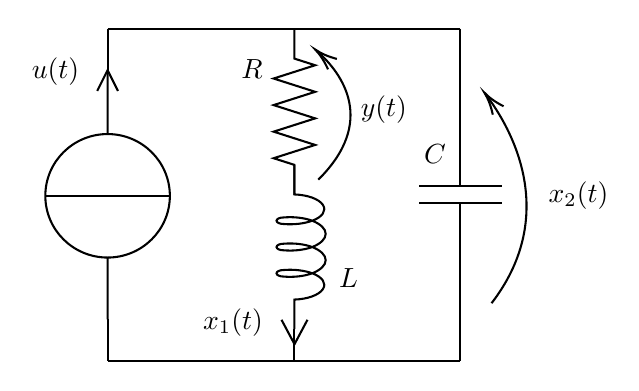
\begin{tikzpicture}[x=0.75pt,y=0.75pt,yscale=-1,xscale=1]
%uncomment if require: \path (0,300); %set diagram left start at 0, and has height of 300

%Shape: Inductor (Air Core) [id:dp2170205039419545] 
\draw   (360,125.6) -- (360,139.85) .. controls (366.36,140.05) and (371.8,142.03) .. (373.7,144.83) .. controls (375.6,147.63) and (373.58,150.68) .. (368.61,152.51) .. controls (364.72,153.92) and (359.71,154.5) .. (354.84,154.09) .. controls (352.94,154.09) and (351.39,153.38) .. (351.39,152.51) .. controls (351.39,151.64) and (352.94,150.93) .. (354.84,150.93) .. controls (359.71,150.52) and (364.72,151.1) .. (368.61,152.51) .. controls (372.74,154.16) and (375.08,156.45) .. (375.08,158.84) .. controls (375.08,161.24) and (372.74,163.53) .. (368.61,165.18) .. controls (364.72,166.59) and (359.71,167.17) .. (354.84,166.76) .. controls (352.94,166.76) and (351.39,166.05) .. (351.39,165.18) .. controls (351.39,164.3) and (352.94,163.59) .. (354.84,163.59) .. controls (359.71,163.18) and (364.72,163.76) .. (368.61,165.18) .. controls (372.74,166.82) and (375.08,169.11) .. (375.08,171.51) .. controls (375.08,173.9) and (372.74,176.19) .. (368.61,177.84) .. controls (364.72,179.25) and (359.71,179.83) .. (354.84,179.42) .. controls (352.94,179.42) and (351.39,178.71) .. (351.39,177.84) .. controls (351.39,176.97) and (352.94,176.26) .. (354.84,176.26) .. controls (359.71,175.85) and (364.72,176.43) .. (368.61,177.84) .. controls (373.58,179.67) and (375.6,182.72) .. (373.7,185.52) .. controls (371.8,188.32) and (366.36,190.3) .. (360,190.5) -- (360,204.75) ;
%Shape: Capacitor [id:dp4914023614500189] 
\draw   (440,100) -- (440,136) (460,144) -- (420,144) (460,136) -- (420,136) (440,144) -- (440,180) ;
%Shape: Resistor [id:dp34404954031853974] 
\draw   (360,60) -- (360,74.4) -- (370,77.6) -- (350,84) -- (370,90.4) -- (350,96.8) -- (370,103.2) -- (350,109.6) -- (370,116) -- (350,122.4) -- (360,125.6) -- (360,140) ;
%Shape: Output [id:dp627431970828664] 
\draw   (270,110.75) .. controls (286.57,110.75) and (300,124.07) .. (300,140.5) .. controls (300,156.93) and (286.57,170.25) .. (270,170.25) .. controls (253.43,170.25) and (240,156.93) .. (240,140.5) .. controls (240,124.07) and (253.43,110.75) .. (270,110.75) -- cycle (270,81) -- (270,110.75) (270,200) -- (270,170.25) ;
%Straight Lines [id:da5613798763631794] 
\draw    (270,60) -- (270,81) ;
%Straight Lines [id:da09203939477984224] 
\draw    (270,200) -- (270,220) ;
%Straight Lines [id:da75524514618233] 
\draw    (440,180) -- (440,220) ;
%Straight Lines [id:da25208752268104473] 
\draw    (440,60) -- (440,100) ;
%Straight Lines [id:da016416307675916175] 
\draw    (270,60) -- (440,60) ;
%Straight Lines [id:da3233048946292705] 
\draw    (270,220) -- (440,220) ;
%Straight Lines [id:da9783234387352633] 
\draw    (240,140.5) -- (300,140.5) ;
\draw   (265,90) -- (270,80) -- (275,90) ;
%Curve Lines [id:da17294524755373375] 
\draw    (371.5,132.75) .. controls (399.82,104.67) and (382.98,81.66) .. (371.41,71.24) ;
\draw [shift={(370,70)}, rotate = 40.29] [color={rgb, 255:red, 0; green, 0; blue, 0 }  ][line width=0.75]    (10.93,-3.29) .. controls (6.95,-1.4) and (3.31,-0.3) .. (0,0) .. controls (3.31,0.3) and (6.95,1.4) .. (10.93,3.29)   ;
\draw   (366.3,200.25) -- (360.05,212) -- (353.8,200.25) ;
%Straight Lines [id:da4376747318657973] 
\draw    (360,204.75) -- (360,220.25) ;
%Curve Lines [id:da28035859406326946] 
\draw    (455,192.25) .. controls (485.71,152.27) and (467.94,112.78) .. (452.67,92.29) ;
\draw [shift={(451.5,90.75)}, rotate = 52.22] [color={rgb, 255:red, 0; green, 0; blue, 0 }  ][line width=0.75]    (10.93,-3.29) .. controls (6.95,-1.4) and (3.31,-0.3) .. (0,0) .. controls (3.31,0.3) and (6.95,1.4) .. (10.93,3.29)   ;

% Text Node
\draw (232,72.4) node [anchor=north west][inner sep=0.75pt]    {$u( t)$};
% Text Node
\draw (333,73.4) node [anchor=north west][inner sep=0.75pt]    {$R$};
% Text Node
\draw (390.5,90.9) node [anchor=north west][inner sep=0.75pt]    {$y( t)$};
% Text Node
\draw (314.5,193.4) node [anchor=north west][inner sep=0.75pt]    {$x_{1}( t)$};
% Text Node
\draw (380,173.9) node [anchor=north west][inner sep=0.75pt]    {$L$};
% Text Node
\draw (421,114.4) node [anchor=north west][inner sep=0.75pt]    {$C$};
% Text Node
\draw (481,132.4) node [anchor=north west][inner sep=0.75pt]    {$x_{2}( t)$};


\end{tikzpicture}


\end{figure}\FloatBarrier

Vigono le Leggi di Kirkhoff e le relazioni costitutive di induttore, resistore e condensatore. Ricaviamo quindi il sistema dinamico:
\begin{equation*}
	\begin{cases}
		\dot{x}_1 (t)=\frac{1}{L}(x_2 (t)-Rx_1 (t)) \\
		\dot{x}_2 (t)=\frac{1}{C}(u(t)-x_1 (t)) \\
        y(t)=Rx_1(t)
	\end{cases}
\end{equation*}

\section{Sistemi a tempo discreto}

Un'equazione alle differenze è del tipo
\begin{equation*}
	x(t+1) =f(x(t) ,u(t)) ,\ t=0,1,2,\dotsc 
\end{equation*}
\textit{Esempio (scuola media)}

\begin{figure}[htpb]\centering


\tikzset{every picture/.style={line width=0.75pt}} %set default line width to 0.75pt        

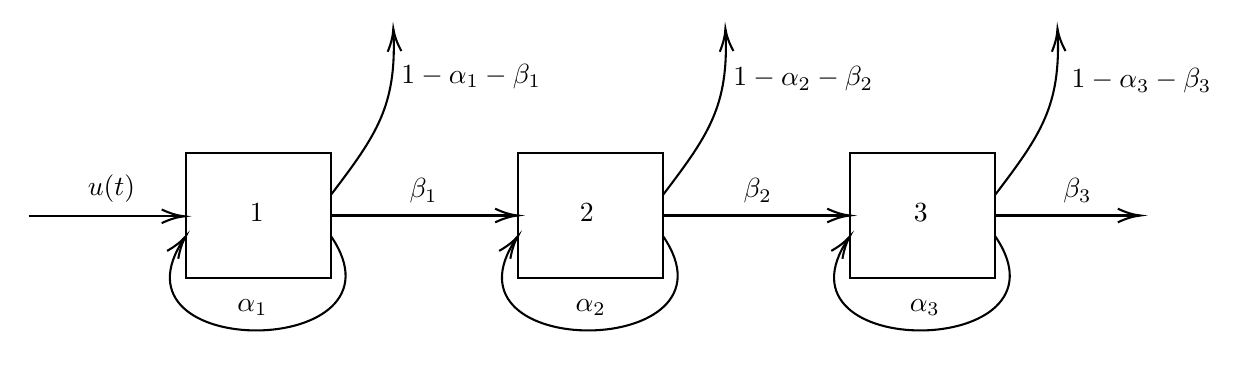
\begin{tikzpicture}[x=0.75pt,y=0.75pt,yscale=-1,xscale=1]
%uncomment if require: \path (0,163); %set diagram left start at 0, and has height of 163

%Shape: Rectangle [id:dp9078246576272557] 
\draw   (135.66,68) -- (205.66,68) -- (205.66,128) -- (135.66,128) -- cycle ;
%Shape: Rectangle [id:dp16146430765594877] 
\draw   (295.66,68) -- (365.66,68) -- (365.66,128) -- (295.66,128) -- cycle ;
%Shape: Rectangle [id:dp20157620405802412] 
\draw   (455.66,68) -- (525.66,68) -- (525.66,128) -- (455.66,128) -- cycle ;
%Straight Lines [id:da08489054860404721] 
\draw    (205.66,98) -- (293.66,98) ;
\draw [shift={(295.66,98)}, rotate = 180] [color={rgb, 255:red, 0; green, 0; blue, 0 }  ][line width=0.75]    (10.93,-3.29) .. controls (6.95,-1.4) and (3.31,-0.3) .. (0,0) .. controls (3.31,0.3) and (6.95,1.4) .. (10.93,3.29)   ;
%Straight Lines [id:da24492953447403631] 
\draw    (365.66,98) -- (453.66,98) ;
\draw [shift={(455.66,98)}, rotate = 180] [color={rgb, 255:red, 0; green, 0; blue, 0 }  ][line width=0.75]    (10.93,-3.29) .. controls (6.95,-1.4) and (3.31,-0.3) .. (0,0) .. controls (3.31,0.3) and (6.95,1.4) .. (10.93,3.29)   ;
%Curve Lines [id:da013142910657578333] 
\draw    (205.66,108) .. controls (246.45,167.7) and (94.19,168.99) .. (135.03,108.91) ;
\draw [shift={(135.66,108)}, rotate = 125.18] [color={rgb, 255:red, 0; green, 0; blue, 0 }  ][line width=0.75]    (10.93,-3.29) .. controls (6.95,-1.4) and (3.31,-0.3) .. (0,0) .. controls (3.31,0.3) and (6.95,1.4) .. (10.93,3.29)   ;
%Curve Lines [id:da7007104386948352] 
\draw    (365.66,108) .. controls (406.45,167.7) and (254.19,168.99) .. (295.03,108.91) ;
\draw [shift={(295.66,108)}, rotate = 125.18] [color={rgb, 255:red, 0; green, 0; blue, 0 }  ][line width=0.75]    (10.93,-3.29) .. controls (6.95,-1.4) and (3.31,-0.3) .. (0,0) .. controls (3.31,0.3) and (6.95,1.4) .. (10.93,3.29)   ;
%Curve Lines [id:da16073059503423237] 
\draw    (525.66,108) .. controls (566.45,167.7) and (414.19,168.99) .. (455.03,108.91) ;
\draw [shift={(455.66,108)}, rotate = 125.18] [color={rgb, 255:red, 0; green, 0; blue, 0 }  ][line width=0.75]    (10.93,-3.29) .. controls (6.95,-1.4) and (3.31,-0.3) .. (0,0) .. controls (3.31,0.3) and (6.95,1.4) .. (10.93,3.29)   ;
%Curve Lines [id:da1216714632497331] 
\draw    (205.66,88) .. controls (227.33,59.43) and (237.35,45.42) .. (235.74,9.65) ;
\draw [shift={(235.66,8)}, rotate = 86.91] [color={rgb, 255:red, 0; green, 0; blue, 0 }  ][line width=0.75]    (10.93,-3.29) .. controls (6.95,-1.4) and (3.31,-0.3) .. (0,0) .. controls (3.31,0.3) and (6.95,1.4) .. (10.93,3.29)   ;
%Curve Lines [id:da2014229271241712] 
\draw    (365.66,88) .. controls (387.33,59.43) and (397.35,45.42) .. (395.74,9.65) ;
\draw [shift={(395.66,8)}, rotate = 86.91] [color={rgb, 255:red, 0; green, 0; blue, 0 }  ][line width=0.75]    (10.93,-3.29) .. controls (6.95,-1.4) and (3.31,-0.3) .. (0,0) .. controls (3.31,0.3) and (6.95,1.4) .. (10.93,3.29)   ;
%Straight Lines [id:da8249160440561312] 
\draw    (525.66,98) -- (593.66,98) ;
\draw [shift={(595.66,98)}, rotate = 180] [color={rgb, 255:red, 0; green, 0; blue, 0 }  ][line width=0.75]    (10.93,-3.29) .. controls (6.95,-1.4) and (3.31,-0.3) .. (0,0) .. controls (3.31,0.3) and (6.95,1.4) .. (10.93,3.29)   ;
%Curve Lines [id:da265661061775639] 
\draw    (525.66,88) .. controls (547.33,59.43) and (557.35,45.42) .. (555.74,9.65) ;
\draw [shift={(555.66,8)}, rotate = 86.91] [color={rgb, 255:red, 0; green, 0; blue, 0 }  ][line width=0.75]    (10.93,-3.29) .. controls (6.95,-1.4) and (3.31,-0.3) .. (0,0) .. controls (3.31,0.3) and (6.95,1.4) .. (10.93,3.29)   ;
%Straight Lines [id:da11133549752389327] 
\draw    (60,98.38) -- (133,98.38) ;
\draw [shift={(135,98.38)}, rotate = 180] [color={rgb, 255:red, 0; green, 0; blue, 0 }  ][line width=0.75]    (10.93,-3.29) .. controls (6.95,-1.4) and (3.31,-0.3) .. (0,0) .. controls (3.31,0.3) and (6.95,1.4) .. (10.93,3.29)   ;

% Text Node
\draw (87,76.78) node [anchor=north west][inner sep=0.75pt]    {$u( t)$};
% Text Node
\draw (159,136.78) node [anchor=north west][inner sep=0.75pt]    {$\alpha _{1}$};
% Text Node
\draw (483,136.78) node [anchor=north west][inner sep=0.75pt]    {$\alpha _{3}$};
% Text Node
\draw (322,136.78) node [anchor=north west][inner sep=0.75pt]    {$\alpha _{2}$};
% Text Node
\draw (242,78.78) node [anchor=north west][inner sep=0.75pt]    {$\beta _{1}$};
% Text Node
\draw (557,78.78) node [anchor=north west][inner sep=0.75pt]    {$\beta _{3}$};
% Text Node
\draw (403,78.78) node [anchor=north west][inner sep=0.75pt]    {$\beta _{2}$};
% Text Node
\draw (238,23.78) node [anchor=north west][inner sep=0.75pt]    {$1-\alpha _{1} -\beta _{1}$};
% Text Node
\draw (398,24.78) node [anchor=north west][inner sep=0.75pt]    {$1-\alpha _{2} -\beta _{2}$};
% Text Node
\draw (561,25.78) node [anchor=north west][inner sep=0.75pt]    {$1-\alpha _{3} -\beta _{3}$};
% Text Node
\draw (165,90.78) node [anchor=north west][inner sep=0.75pt]    {$1$};
% Text Node
\draw (324,90.78) node [anchor=north west][inner sep=0.75pt]    {$2$};
% Text Node
\draw (485,90.78) node [anchor=north west][inner sep=0.75pt]    {$3$};


\end{tikzpicture}

\end{figure}\FloatBarrier

È un sistema compartimentale. Come transitano gli individui da un sistema all'altro? Ho 3 compartimenti
\begin{equation*}
	\begin{cases}
		x_1 (t+1)=\alpha _1 x_1 (t)+u(t)             \\
		x_2 (t+1)=\alpha _2 x_2 (t)+\beta _1 x_1 (t) \\
		x_3 (t+1)=\alpha _3 x_3 (t)+\beta _2 x_2 (t) \\
        y(t)=x_1(t)+x_2(t)+x_3(t)
	\end{cases}
\end{equation*}
$y(t)$ rappresenta il totale degli studenti, ma posso essere interessato a diverse quantità.

La forma generale è
\begin{equation*}
	\boxed{
		\begin{cases}
			x(t+1)=f(x(t),u(t)) \\
			y(t)=g(x(t),u(t))  
		\end{cases}
	}
\end{equation*}
La $u(t)$ nella $y$ c'è in pochissimi modelli, il sistema si dice \textbf{improprio} ed è quasi sempre figlia di semplificazioni modellistiche.
Scriviamo i vettori
\begin{equation*}
	u(t)=\begin{bmatrix}
	u_1 (t)\\
	u_2 (t)\\
	\vdots \\
	u_m (t)
	\end{bmatrix} \in \mathbb{R}^m ,\ \ y(t)=\begin{bmatrix}
	y_1 (t)\\
	y_2 (t)\\
	\vdots \\
	y_q (t)
	\end{bmatrix} \in \mathbb{R}^q ,\ \ x(t)=\begin{bmatrix}
	x_1 (t)\\
	x_2 (t)\\
	\vdots \\
	x_n (t)
	\end{bmatrix} \in \mathbb{R}^n
\end{equation*}
$n$ è l'ordine del sistema.

Se $m=1,q=1$ il sistema è \textit{SISO} (single input single output), studieremo questi. Altrimenti è \textit{MIMO} (multi input multi output).

Siano dati
\begin{itemize}
	\item $\dot{x}(t) =f(x(t) ,u(t))$ con $f$ abbastanza regolare
	\item lo stato iniziale $x(0)$
	\item un ingresso applicato $u(\tau) ,0\leq \tau < t$
\end{itemize}

Allora $\exists !\ x(\tau) ,0\leq \tau < t,\exists !\ y(\tau) =g(x(\tau) ,u(\tau))$ e possiamo estendere $t$ quanto vogliamo. Discorso analogo per quelli a tempo discreto. Per trovare la soluzione ci servono solo lo stato iniziale e l'ingresso applicato.

\section{Linearità}

Un sistema a tempo continuo è lineare se
\begin{align*}
	\dot{x}_1 & =f_1(x_1 ,x_2 ,\dotsc ,x_n ,u) =a_{11} x_1 +a_{12} x_2 +\cdots +a_{1n} x_n +b_1 u \\
	\dot{x}_2 & =f_2(x_1 ,x_2 ,\dotsc ,x_n ,u) =a_{21} x_1 +a_{22} x_2 +\cdots +a_{2n} x_n +b_2 u \\
	\vdots    &                                                                                    \\
	\dot{x}_n & =f_n(x_1 ,x_2 ,\dotsc ,x_n ,u) =a_{n1} x_1 +a_{n2} x_2 +\cdots +a_{nn} x_n +b_n u \\
	y(t)      & =g(x(t),u(t))=c_1 x_1 +c_2 x_2 +\cdots +c_n x_n +du                               
\end{align*}
Ovvero scriviamo tutto come
\begin{gather*}
	\boxed{
		\begin{aligned}
			\dot{x}(t) & =Ax(t) +bu(t) \\
			y(t)       & =cx(t) +du(t) 
		\end{aligned}
		}\\
	\\
	\begin{array}{ l l }
		A=\begin{bmatrix}
		a_{11} & \cdots & a_{1n} \\
		\vdots & \ddots & \vdots \\
		a_{n1} & \cdots & a_{nn} 
		\end{bmatrix} \in \mathbb{R}^{n\times n} & b=\begin{bmatrix}
		b_1\\
		\vdots \\
		b_n
		\end{bmatrix} \in \mathbb{R}^{n\times 1}\\
		c=\begin{bmatrix}
		c_1    & \cdots & c_n    
		\end{bmatrix} \in \mathbb{R}^{1\times n} & d=\begin{bmatrix}
		d
		\end{bmatrix}
	\end{array} \ \ 
\end{gather*}
Un sistema a tempo discreto è lineare se
\begin{align*}
	x_1(t+1) & =a_{11} x_1(t) +a_{12} x_2(t) +\cdots +a_{1n} x_n(t) +b_1 u(t) \\
	x_2(t+1) & =a_{21} x_1(t) +a_{22} x_2(t) +\cdots +a_{2n} x_n(t) +b_2 u(t) \\
	\vdots    &                                                                \\
	x_n(t+1) & =a_{n1} x_1(t) +a_{n2} x_2(t) +\cdots +a_{nn} x_n(t) +b_n u(t) \\
	y(t)      & =c_1 x_1(t) +c_2 x_2(t) +\cdots +c_n x_n(t) +du(t)             
\end{align*}
Ovvero scriviamo tutto come
\begin{equation*}
	\boxed{
		\begin{aligned}
			x(t+1) & =Ax(t) +bu(t) \\
			y(t)    & =cx(t) +du(t) 
		\end{aligned} \ \ }
\end{equation*}

\chapter{Modello interno}

\section{Movimento e traiettoria}

Il \textbf{movimento} è una funzione a valori vettoriali, in particolare è la soluzione del vettore di stato $x(t)$.

Ipotizzando che il sistema sia di ordine $2$, il grafico della traiettoria è una curva di $\mathbb R^3$ che mostra l'andamento di $x_1$ e $x_2$ nel tempo.


\begin{figure}[htpb]\centering


\tikzset{every picture/.style={line width=0.75pt}} %set default line width to 0.75pt        



\tikzset{every picture/.style={line width=0.75pt}} %set default line width to 0.75pt        

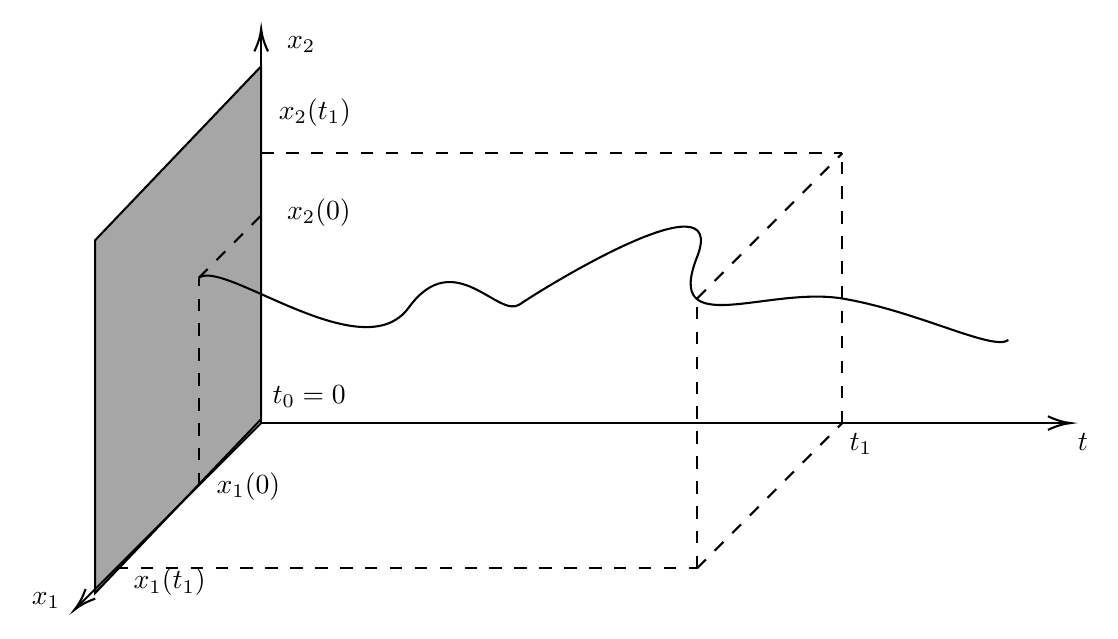
\begin{tikzpicture}[x=0.75pt,y=0.75pt,yscale=-1,xscale=1]
%uncomment if require: \path (0,300); %set diagram left start at 0, and has height of 300

%Straight Lines [id:da3055123061955123] 
\draw    (180,190) -- (91.41,278.59) ;
\draw [shift={(90,280)}, rotate = 315] [color={rgb, 255:red, 0; green, 0; blue, 0 }  ][line width=0.75]    (10.93,-3.29) .. controls (6.95,-1.4) and (3.31,-0.3) .. (0,0) .. controls (3.31,0.3) and (6.95,1.4) .. (10.93,3.29)   ;
%Straight Lines [id:da1482030458017568] 
\draw    (180,190) -- (568,190) ;
\draw [shift={(570,190)}, rotate = 180] [color={rgb, 255:red, 0; green, 0; blue, 0 }  ][line width=0.75]    (10.93,-3.29) .. controls (6.95,-1.4) and (3.31,-0.3) .. (0,0) .. controls (3.31,0.3) and (6.95,1.4) .. (10.93,3.29)   ;
%Straight Lines [id:da04774733935961384] 
\draw    (180,190) -- (180,2) ;
\draw [shift={(180,0)}, rotate = 90] [color={rgb, 255:red, 0; green, 0; blue, 0 }  ][line width=0.75]    (10.93,-3.29) .. controls (6.95,-1.4) and (3.31,-0.3) .. (0,0) .. controls (3.31,0.3) and (6.95,1.4) .. (10.93,3.29)   ;
%Shape: Rectangle [id:dp9465354860663429] 
\draw  [fill={rgb, 255:red, 0; green, 0; blue, 0 }  ,fill opacity=0.35 ] (180,18.1) -- (180,188.1) -- (100,271.9) -- (100,101.9) -- cycle ;
%Curve Lines [id:da17612402023901086] 
\draw    (150,120) .. controls (162.19,110.85) and (229,164.73) .. (251.06,134.4) .. controls (273.12,104.06) and (294.28,140.07) .. (304.56,132.84) .. controls (314.85,125.62) and (406,69.27) .. (390,110) .. controls (374,150.73) and (423.75,123.97) .. (460,130) .. controls (496.25,136.03) and (532.64,155.52) .. (540,150) ;
%Straight Lines [id:da10729910403508991] 
\draw  [dash pattern={on 4.5pt off 4.5pt}]  (150,120) -- (180,90) ;
%Straight Lines [id:da3382406164182523] 
\draw  [dash pattern={on 4.5pt off 4.5pt}]  (150,220) -- (150,120) ;
%Straight Lines [id:da542548455022142] 
\draw  [dash pattern={on 4.5pt off 4.5pt}]  (390,260) -- (390,130) ;
%Straight Lines [id:da9382200126193075] 
\draw  [dash pattern={on 4.5pt off 4.5pt}]  (390,260) -- (460,190) ;
%Straight Lines [id:da9071862164708364] 
\draw  [dash pattern={on 4.5pt off 4.5pt}]  (110,260) -- (390,260) ;
%Straight Lines [id:da9783091853808411] 
\draw  [dash pattern={on 4.5pt off 4.5pt}]  (460,190) -- (460,60) ;
%Straight Lines [id:da8399278200224751] 
\draw  [dash pattern={on 4.5pt off 4.5pt}]  (390,130) -- (460,60) ;
%Straight Lines [id:da8610859099553595] 
\draw  [dash pattern={on 4.5pt off 4.5pt}]  (180,60) -- (460,60) ;

% Text Node
\draw (572,193.4) node [anchor=north west][inner sep=0.75pt]    {$t$};
% Text Node
\draw (68,270.3) node [anchor=north west][inner sep=0.75pt]    {$x_{1}$};
% Text Node
\draw (191,2.4) node [anchor=north west][inner sep=0.75pt]    {$x_{2}$};
% Text Node
\draw (117,258.4) node [anchor=north west][inner sep=0.75pt]    {$x_{1}( t_{1})$};
% Text Node
\draw (157,212.4) node [anchor=north west][inner sep=0.75pt]    {$x_{1}( 0)$};
% Text Node
\draw (187,32.4) node [anchor=north west][inner sep=0.75pt]    {$x_{2}( t_{1})$};
% Text Node
\draw (191,80.4) node [anchor=north west][inner sep=0.75pt]    {$x_{2}( 0)$};
% Text Node
\draw (462,193.4) node [anchor=north west][inner sep=0.75pt]    {$t_{1}$};
% Text Node
\draw (184,170.4) node [anchor=north west][inner sep=0.75pt]    {$t_{0} =0$};
\end{tikzpicture}

\end{figure}\FloatBarrier

Definiamo lo spazio di stato come l'insieme su cui assume valori $x(t)$. Per un sistema di ordine $2$, nel grafico sopra è rappresentato in grigio lo spazio di stato.

La \textbf{traiettoria} è il movimento proiettato sullo spazio di stato. In altre parole, se immaginassimo di guardare il grafico del movimento con la $t$ uscente, quella che vedremmo sarebbe la traiettoria.

Se $u(t) =\overline{u} \ \forall t\geq 0$, cioè l'ingresso è costante, non si intersecano le traiettorie.

Supponendo $u(t) =\overline{u} \ \forall t\geq 0$, consideriamo sistemi lineari del tipo
\begin{gather*}
	\dot{x} (t)=Ax(t)+bu(t)\\
	x(t+1)=Ax(t)+bu(t)
\end{gather*}

\section{Equilibrio: esistenza e unicità}

\begin{defn}
	Si dice che $\overline{x} \in \mathbb{R}^n$ è un equilibrio se $x(0) =\overline{x} \implies x(t) =\overline{x} \ \forall t\geq 0$.
\end{defn}
Ovvero, se è in uno stato e poi ci rimane per sempre, quello è uno stato di equilibrio. Esistono tanti tipi di situazioni di questo tipo.

A tempo continuo l'equilibrio si traduce in
\begin{equation*}
	0=\dot{x} (t)=A\underbrace{x(t)}_{\overline{x}} +bu(t)\implies A\overline{x} =-b\overline{u}
\end{equation*}
È un sistema lineare, ricordiamo quindi i risultati di Rouche-Capelli-Cramer
\begin{enumerate}
	\item se $\det A\neq 0\implies \exists A^{-1}$ e $\boxed{\overline{x} =-A^{-1} b\overline{u}}$
	\item se $\det A=0\implies \nexists A^{-1}$
	      \begin{enumerate}
	      	\item $\nexists \overline{x}$, non esiste nessuno stato di equilibrio
	      	\item $\exists \infty \overline{x}$, esistono infiniti equilibri
	      \end{enumerate}
\end{enumerate}
\begin{defn}
	Si dice \textbf{guadagno} la quantità $\mu $
	\begin{equation*}
		\overline{y} =\mu \overline{u} \ \ \implies \ \ \boxed{\mu =\frac{\overline{y}}{\overline{u}}}
	\end{equation*}
\end{defn}
La si può ricavare dalle relazioni del sistema a tempo continuo in questo modo
\begin{equation*}
	\begin{aligned}
		\overline{y} & =c\overline{x} +d\overline{u}           \\
		             & =-cA^{-1} b\overline{u} +d\overline{u}  \\
		             & =\left(-cA^{-1} b+d\right)\overline{u} 
	\end{aligned} \ \ \implies \ \ \boxed{\mu =-cA^{-1} b+d}
\end{equation*}

Nel caso a tempo discreto l'equilibrio significa
\begin{equation*}
	\overline{x} =A\overline{x} +b\overline{u} \implies I\overline{x} -A\overline{x} =b\overline{u} \implies (I-A)\overline{x} =b\overline{u}
\end{equation*}
È un sistema lineare, valgono gli stessi risultati di prima:
\begin{enumerate}
	\item se $\det(I-A) \neq 0\implies \exists (I-A)^{-1}$ e $\boxed{\overline{x} =(I-A)^{-1} b\overline{u}}$
	\item se $\det(I-A) =0\implies \nexists (I-A)^{-1}$
	      \begin{enumerate}
	      	\item $\nexists \overline{x}$, non esiste nessuno stato di equilibrio
	      	\item $\exists \infty \overline{x}$, esistono infiniti equilibri
	      \end{enumerate}
\end{enumerate}

Mentre per il guadagno è (si noti che è diverso dal caso a tempo continuo)
\begin{equation*}
	\begin{aligned}
		\overline{y} & =c\overline{x} +d\overline{u}               \\
		             & =c(I-A)^{-1} b\overline{u} +d\overline{u}  \\
		             & =\left(c(I-A)^{-1} b+d\right)\overline{u} 
	\end{aligned} \ \ \implies \ \ \boxed{\mu =c(I-A)^{-1} b+d}
\end{equation*}
Nota: nei casi in cui le matrici (rispettivamente $A$ nel caso continuo e $(I-A)$ nel caso discreto) non siano invertibili, \textbf{il guadagno non è definito}.

\section{Casi critici}

\begin{rem}
	Data una qualunque matrice quadrata $A$, il determinante è uguale al prodotto degli autovalori:
	\begin{equation*}
		\det A=\prod ^n_{i=1} \lambda _i
	\end{equation*}
\end{rem}
Quindi:
\begin{itemize}
	\item tempo continuo: $\det A=0\iff \exists \lambda _i =0$ (se ne esiste almeno uno nullo)
	\item tempo discreto: $\det(I-A) =0\iff \exists \lambda _i =1$ (se ne esiste almeno uno unitario)
\end{itemize}

\section{Formula di Lagrange e sovrapposizione degli effetti}

Nei sistemi dinamici lineari a tempo continuo abbiamo già detto che il movimento è univocamente determinato. Vale allora la formula di Lagrange, la quale ci dice che il movimento è separabile in due fattori additivi, movimento libero e movimento forzato:
\begin{equation}
	\boxed{
		\begin{aligned}
			{\displaystyle x(t)} & {\displaystyle =e^{At} x(0) +\int ^t_0 e^{A(t-\tau)} bu(\tau) d\tau } \\
			                     & =\phi (t) x(0) +\psi (t) \left(u_{[ 0,t)}\right)                                             \\
			                     & =x_L(t) +x_F(t)                                                                  
		\end{aligned}
	}
\end{equation}
Ricordiamo che il termine ${\displaystyle e^{At}}$ vale
\begin{equation*}
	{\displaystyle e^{At} =I+At+\frac{1}{2!} A^2 t^2 +\frac{1}{3!} A^3 t^3 \dotsc =\sum\limits ^{\infty }_{k=1}\frac{A^k t^k}{k!} =\phi (t)}
\end{equation*}
ed è detto \textbf{matrice di transizione}. Non si pone il problema di convergenza della serie, in quanto si ha che ciò è garantito qualunque siano $A,t$.

Il \textbf{movimento libero} è quello che abbiamo se il sistema funziona ad ingresso $u=0$.

Il \textbf{movimento forzato} è quello che osserviamo se il sistema parte dallo stato iniziale $x(0) =0$.
\begin{thm}
	[Sovrapposizione di cause-effetti]
	\begin{equation*}
		\begin{drcases}
			x_1(0)\\
			u_1(t)
		\end{drcases} \implies x_1(t) \ \ \ \ \begin{drcases}
		x_2(0)\\
		u_2(t)
		\end{drcases} \implies x_2(t)
	\end{equation*}
	Allora
	\begin{equation*}
		\begin{drcases}
			x_3(0) =\alpha x_1(0) +\beta x_2(0)\\
			u_3(t) =\alpha u_1(t) +\beta u_2(t)
		\end{drcases} \implies x_3(t) =\alpha x_1(t) +\beta x_2(t)
	\end{equation*}
\end{thm}
\begin{rem}
	Una matrice $A\in \mathbb{R}^{n\times n}$ si dice \textbf{nilpotente} se ha tutti gli autovalori nulli, in particolare in tal caso si ha $A^n =0$.
\end{rem}
\textbf{Formula di Lagrange per sistemi a tempo discreto.} Il caso discreto è più facile da trattare e si può ricavare a partire da $x(t+1)=Ax(t)+bu(t)$
\begin{equation*}
	\begin{aligned}
		x(0) &                                                   \\
		x(1) & =Ax(0) +bu(0)                                     \\
		x(2) & =Ax(1) +bu(1) =A^2 x(0) +Abu(0) +bu(1)            \\
		x(3) & =Ax(2) +bu(2) =A^3 x(0) +A^2 bu(0) +Abu(1) +bu(2) 
	\end{aligned}
\end{equation*}
Allora
\begin{equation}
	\boxed{
		\begin{aligned}
			x(t) & =A^t x(0) +\sum\limits ^{t-1}_{i=0} A^{t-i-1} bu(i) \\
			     & =\phi (t) x(0) +\psi (t)_{u[ 0,t)}                  \\
			     & =x_L(t) +x_F(t)                                     
		\end{aligned}
	}
\end{equation}

\section{Modello esterno e funzione di trasferimento}

Per i sistemi a tempo continuo, introduciamo l'operatore $s$ (trasformata di Laplace)
\begin{equation*}
	\frac{dv(t)}{dt} =sv,\ \ \ \ \frac{d^2 v(t)}{dt^2} =s^2 v,\dotsc ,\ \ \ \ \frac{d^k v(t)}{dt^k} =s^k v,\ \ 
\end{equation*}
Il modello esterno esprime la relazione tra l'ingresso e l'uscita usando un polinomio dipendente da $s$.
\begin{equation*}
	D(s) y=N(s) u
\end{equation*}
Si può poi definire la funzione di trasferimento
\begin{equation*}
	\boxed{G(s) =\frac{N(s)}{G(s)}}
\end{equation*}
A tempo discreto si introduce la trasformata zeta, codifica lo \textit{shift} del segnale
\begin{equation*}
	v(t+1) =zv,\ \ \ \ v(t+2) =z^2 v,\dotsc ,\ \ \ \ v(t+k) =z^k v
\end{equation*}
Quindi riassumendo entrambi i casi:
\begin{itemize}
	\item t. continuo\begin{equation*}
	      \begin{cases}
	      	\dot{x} =Ax+bu \\
	      	y=cx+du        
	      \end{cases} \ \ \implies \ \ \begin{cases}
	      sx=Ax+bu\\
	      y=cx+du
	\end{cases}
	\end{equation*}
	\item t. discreto\begin{equation*}
	      \begin{cases}
	      	x(t+1)=Ax(t)+bu(t) \\
	      	y(t)=cx(t)+du(t)   
	      \end{cases} \ \ \implies \ \ \begin{cases}
	      zx=Ax+bu\\
	      y=cx+du
	\end{cases}
	\end{equation*}
\end{itemize}

Sviluppiamo il caso continuo
\begin{equation*}
	\begin{cases}
		(sI-A)x=bu \\
		y=cx+du    
	\end{cases}
\end{equation*}
Se $\det(sI-A) \neq 0$
\begin{equation*}
	\begin{cases}
		x=(sI-A)^{-1} bu                                       \\
		y=\underbrace{\left[ c(sI-A)^{-1} b+d\right]}_{G(s)} u 
	\end{cases}
\end{equation*}
Vediamo com'è fatta $(sI-A)^{-1}$, sappiamo che al denominatore c'è il polinomio caratteristico di $A$ calcolato in $s$, che moltiplica $P(s)$, cioè una matrice di polinomi in $s$ di grado $< n$ strettamente. Il polinomio caratteristico ha grado $n$.
\begin{equation*}
	(sI-A)^{-1} =\frac{P(s)}{\Delta _A(s)}
\end{equation*}
Sostituiamola in $y$
\begin{equation*}
	y=\left[ c\frac{P(s)}{\Delta _A(s)} b+d\right] u=\left[\frac{cP(s) b+d\Delta _A(s)}{\Delta _A(s)}\right] u=G(s) u
\end{equation*}
Il grado di $cP(s) b$ è $< n$, mentre il grado di $d\Delta _A(s)$ è $n$. Di conseguenza il grado del numeratore complessivo è $n\iff d\neq 0$ (sistema improprio), mentre è strettamente minore di $n\iff d=0$. Scriviamo quindi la funzione di trasferimento come rapporto di polinomi.
\begin{equation*}
	G(s) =\frac{N(s)}{D(s)} =\frac{N(s)}{\Delta _A(s)} =\frac{\beta _0 s^n +\beta _1 s^{n-1} +\cdots +\beta _n}{s^n +\alpha _1 s^{n-1} +\cdots +\alpha _n}
\end{equation*}
Il denominatore ha sempre grado $n$, mentre il numeratore ha grado $\leq n$. Indichiamo con $\beta _m$ il primo coefficiente non nullo.
\begin{equation*}
	G(s) =\frac{\beta _m s^{n-m} +\cdots +\beta _n}{s^n +\alpha _1 s^{n-1} +\cdots +\alpha _n}
\end{equation*}
e fattorizziamo questi polinomi
\begin{equation}
	G(s) =\frac{\beta _m(s-q_1)(s-q_2) \cdots (s-q_{n-m})}{(s-p_1)(s-p_2) \cdots (s-p_n)}\begin{array}{ l }
	\implies \ \text{zeri}\\
	\implies \ \text{poli}
	\end{array}
\end{equation}
I $p_i$ sono le radici del denominatore e sono dette \textbf{poli}, i $q_i$ sono le radici del numeratore e sono detti \textbf{zeri}. Se dovessero esserci poli e zeri uguali, ci sarebbe una terrificante semplificazione e perdita di grado.

Notiamo infine un risultato importante:
\begin{equation*}
	\begin{array}{|l c|}
		\hline
		\text{t. continuo:} & \mu =G(0) \\
		\hline
		\text{t. discreto:} & \mu =G(1) \\
		\hline
	\end{array}
\end{equation*}
Nel caso continuo, questo risultato non vale se $s=0$ è un polo, cioè è a denominatore, infatti si dividerebbe per $0$; anche in questo caso \textbf{il guadagno non è definito}. Analogamente si ragiona per il caso discreto.

\section{Problema della realizzazione}

Da modello interno $(A,b,c,d)$ a esterno $(G(s))$ il passaggio è univoco $G(s) =c(sI-A)^{-1} b+d$, il passaggio inverso si chiama realizzazione.

Data $G(s)$ la quaterna non è unica. Se ne abbiamo una, qualunque altra ottenuta facendo un cambiamento di base nello spazio di stato è una quaterna valida.
\begin{equation*}
	x=\begin{bmatrix}
	x_1\\
	\vdots \\
	x_n
	\end{bmatrix} \in \mathbb{R}^n \ \ \implies \ \ z=Tx
\end{equation*}
dove $T\in \mathcal{M}(n\times n) ,\det T\neq 0$ e quindi $x=T^{-1} z$.

Le relazioni di stato e uscita del sistema
\begin{gather*}
	\dot{x} =Ax+bu\\
	y=cx+du
\end{gather*}
diventano
\begin{equation*}
	\begin{aligned}
		\dot{z} & =T\dot{x} =T\left(Ax+bu\right) =T\left(AT^{-1} z+bu\right) =TAT^{-1} +Tbu=\tilde{A} z+\tilde{b} u \\
		y       & =c\left(T^{-1} z\right) +du=\tilde{c} z+\tilde{d} u                                                
	\end{aligned}
\end{equation*}
ovvero
\begin{equation*}
	\boxed{\tilde{A} =TAT^{-1} ,\ \ \ \ \tilde{b} =Tb,\ \ \ \ \tilde{c} =cT^{-1} ,\ \ \ \ \tilde{d} =d}
\end{equation*}
Dimostriamo che il sistema originale e quello trasformato hanno la stessa funzione di trasferimento
\begin{equation*}
	\begin{aligned}
		\tilde{G}(s) & =\tilde{c}\left(sI-\tilde{A}\right)^{-1}\tilde{b} +\tilde{d} &                                                  \\
		             & =cT^{-1}\left(sI-TAT^{-1}\right)^{-1} Tb+d                   & \text{(sostituzione)}                            \\
		             & =cT^{-1}\left(s T I T^{-1} -TAT^{-1}\right)^{-1} Tb+d        & \text{(furbata)}                                 \\
		             & =cT^{-1}\left(T(sI-A) T^{-1}\right)^{-1} Tb+d               & \text{(raccoglimento)}                           \\
		             & =cT^{-1} T(sI-A)^{-1} T^{-1} Tb+d                            & \text{(inv. di prod. = prod. di inv. al contr.)} \\
		             & =c(sI-A)^{-1} b+d=G(s)                                       &                                                  
	\end{aligned}
\end{equation*}
Tra tutte le forme, con $d=0$, la forma canonica è
\begin{equation*}
	\begin{aligned}
		A & =\begin{bmatrix}
		0          & 1      &        &            &            \\
		           & 0      & 1      &            &            \\
		           &        & \ddots & \ddots     &            \\
		           &        &        & 0          & 1          \\
		-\alpha _n & \cdots & \cdots & -\alpha _2 & -\alpha _1 
		\end{bmatrix} & b & =\begin{bmatrix}
		0\\
		\vdots \\
		\vdots \\
		0\\
		1
		\end{bmatrix}\\
		c & =\begin{bmatrix}
		\beta _n   & \cdots & \cdots & \beta _2   & \beta _1   
		\end{bmatrix} & d & =\begin{bmatrix}
		0
		\end{bmatrix}
	\end{aligned}
\end{equation*}

\chapter{Stabilità}

Chiamiamo $\Sigma $ il sistema lineare che stiamo studiando. Studiare la stabilità significa chiedersi cosa succede al sistema per $t\to \infty $ quando non si parte dall'equilibrio. Sappiamo dalla formula di Lagrange che la soluzione si può scrivere come somma di movimento libero e movimento forzato:
\begin{equation*}
	x\left(t\right) =x_L\left(t\right) +x_F\left(t\right)=\phi (t) x(0) +\psi (t) \left(u_{[ 0,t)}\right)
\end{equation*}
\textit{La stabilità riguarda solo il movimento libero.}
\begin{enumerate}
	\item $\Sigma $ è \textbf{asintoticamente stabile} se $\lim\limits _{t\to \infty } x_L\left(t\right) = \underline{0}\ \forall x\left(0\right)$, ovvero se $\phi \left(t\right) x\left(0\right)\to \underline{0}$. Tutte le funzioni dentro $\phi \left(t\right)$ devono tendere a $0$, quindi $x\left(t\right)\to x_F\left(t\right)$, si perde la memoria iniziale del sistema.
	\item $\Sigma $ è \textbf{semplicemente stabile} se $x_L\left(t\right) =\phi \left(t\right) x\left(0\right)$ è limitato $\forall x\left(0\right)$ ma esiste almeno un $x\left(0\right)$ per cui $\phi \left(t\right) x\left(0\right) \nrightarrow \underline{0}$ (il limite o non esiste o non è zero).
	\item $\Sigma $ è \textbf{instabile} se esiste un $x\left(0\right)$ per cui $x_L\left(t\right) =\phi \left(t\right) x\left(0\right)$ è illimitato (diverge).
\end{enumerate}

Queste definizioni generano una partizione fra i tipi di sistemi. \textit{La stabilità non dipende dall'ingresso }$u$\textit{ o da }$b$\textit{, ma solo dalla matrice }$A$\textit{.}
\begin{thm}
	$\Sigma $ asintoticamente stabile se e solo se
	\begin{equation*}
		u\left(t\right) =\overline{u} \ \forall t\geq 0,\ \begin{cases}
		\overline{x} \ \exists !\\
		 \lim\limits _{t\to \infty } x\left(t\right) =\overline{x} \ \forall x\left(0\right)
		\end{cases}
	\end{equation*}
\end{thm}
\textbf{Stabilità a t. continuo con }$n=1$\textbf{ }
\begin{equation*}
	\dot{x} =ax+bu\ \ \implies \ \ x_L\left(t\right) =\phi \left(t\right) x\left(0\right) =e^{at} x\left(0\right)
\end{equation*}
\begin{itemize}
	\item se $a< 0$ è asint. stabile. Se inoltre l'ingresso è costante il valore a equilibrio si trova\begin{equation*}
	      0=a\overline{x} +b\overline{u} \implies \overline{x} =-\frac{b}{a}\overline{u}
	\end{equation*}
	
	Introduciamo la \textbf{costante di tempo a t. continuo}\begin{equation*}
	\boxed{T=-\frac{1}{a}  >0}
	\end{equation*}Dopo circa $5T$ il valore della funzione è meno dell'$1\%$, quindi il \textbf{tempo di risposta} vale\begin{equation*}
	\boxed{T_R \approx 5T=-\frac{5}{a}}
	\end{equation*}
	\item se $a=0$ è sempl. stabile, $x_L\left(t\right) =e^{at} x\left(0\right) =x\left(0\right)$
	\item se $a >0$ è instabile
\end{itemize}

\textbf{Stabilità a t. discreto con} $n=1$
\begin{itemize}
	\item se $\left| a\right| < 1$ è asint. stabile con \textbf{costante di tempo a t. discreto}\begin{equation*}
	      \boxed{T=-\frac{1}{\log\left| a\right| }} \ \ \implies \ \ \boxed{T_R \approx 5T=-\frac{5}{\log\left| a\right| }}
	\end{equation*}
	\item se $\left| a\right| =1$ è sempl. stabile
	\item se $\left| a\right|  >1$ è instabile
\end{itemize}

\textit{In particolare, se }$a< 0$\textit{ ci sono oscillazioni.}

\textbf{Stabilità a t. continuo con }$n\geq 1$\textbf{ generico.} Facciamo l'ipotesi che $A$ sia diagonalizzabile e $\dot{x}\left(t\right) =Ax\left(t\right)$
\begin{equation*}
	x=\begin{bmatrix}
	x_1\\
	\vdots \\
	x_n
	\end{bmatrix} \in \mathbb{R}^n \ \ \ \ z=\begin{bmatrix}
	z_1\\
	\vdots \\
	z_n
	\end{bmatrix} \in \mathbb{R}^n \ \ \ \ z=Tx,\ x=T^{-1} z,\ \det T\neq 0
\end{equation*}
Allora $\dot{z} =\tilde{A} z,\tilde{A} =TAT^{-1}$ e $\sigma \left(A\right) =\sigma \left(\tilde{A}\right)$ con
\begin{equation*}
	\tilde{A} =\begin{bmatrix}
	\lambda _1 &  & \\
	& \ddots  & \\
	&  & \lambda _n
	\end{bmatrix}
\end{equation*}
Una matrice è diagonalizzabile quando ammette $n$ autovettori linearmente indipendenti, cioè quando gli autovalori sono regolari. In particolare la condizione è soddisfatta se gli autovalori sono distinti. Si ha che
\begin{equation*}
	\dot{z} =\tilde{A} z\ \ \iff \ \ \begin{array}{ c }
	\dot{z}_1 =\lambda _1 z_1\\
	\vdots \\
	\dot{z}_n =\lambda _n z_n
	\end{array}
\end{equation*}
sono $n$ sistemi di ordine $1$ che evolvono in maniera indipendente come $z_i\left(t\right) =e^{\lambda _i t} z_i\left(0\right)$. Allora, se $A$ è diagonalizzabile,
\begin{enumerate}
	\item $A$ è asint. stabile $\iff $ $\Re\left(\lambda _i\right) < 0\ \forall i$
	\item $A$ è sempl. stabile $\iff $ $\Re\left(\lambda _i\right) \leq 0\ \forall i,\ \exists i:\Re\left(\lambda _i\right) =0$
	\item $A$ è instabile $\impliedby $ $\exists i:\Re\left(\lambda _i\right)  >0$
\end{enumerate}

Gli autovalori sono le radici del polinomio caratteristico
\begin{equation*}
	\Delta _A\left(\lambda \right) =\Delta _{\tilde{A}}\left(\lambda \right) =\det\left(\lambda I-A\right) =\lambda ^n +\alpha _1 \lambda ^{n-1} +\cdots +\alpha _n
\end{equation*}
Ci può essere un certo $\lambda _i =a+ib$, ma dato che stiamo lavorando con matrici a valori reali in quel caso c'è anche il suo complesso coniugato $\lambda _j =a-ib$ (anche le corrispondenti $z$ sarebbero complesse). Per capire cosa succede, ricordiamo la formula di Eulero
\begin{equation*}
	\begin{aligned}
		z_i\left(t\right) & =e^{\left(a+ib\right) t} z_i\left(0\right) =e^{at} e^{ibt} z_i\left(0\right)    \\
		                   & =e^{at}\left[\cos\left(bt\right) +i\sin\left(bt\right)\right] z_i\left(0\right) 
	\end{aligned}
\end{equation*}
La convergenza è descritta dalla parte reale di $\lambda _i$. Studiamo la coppia coniugata $\lambda _{1,2} =a\pm ib$:
\begin{equation*}
	\gamma _1 e^{\lambda _1 t} +\gamma _2 e^{\lambda _2 t} =\gamma _1 e^{at} e^{ibt} +\gamma _2 e^{at} e^{-ibt} =\dotsc =\alpha e^{at}\left(\sin\left(bt\right) +\beta \right)
\end{equation*}
con $\alpha ,\beta \in \mathbb{R}$. Vale la discussione sul valore del parametro $a$.

La soluzione è una combinazione lineare di esponenziali, pertanto gli esponenziali più lenti sono quelli che governano la risposta. Chiamiamo il \textbf{tempo di risposta dominante}:
\begin{equation*}
	\boxed{T_D =\max_i T_i} \ \ \ \ \boxed{T_R \approx 5T_D}
\end{equation*}
È determinato dall'autovalore più a destra, detto \textbf{autovalore dominante}.

Se gli autovalori dominanti sono una coppia complessa coniugata la costante di tempo vale
\begin{equation*}
	\boxed{T_{1,2} =-\frac{1}{\Re\left(\lambda _{1,2}\right)}}
\end{equation*}
\begin{rem}
	Se $A$ è triangolare a blocchi, il suo spettro è l'unione degli spettri dei blocchi.
	\begin{equation*}
        \left[
            \begin{array}{cc|c}
			        a & b & f \\
			        c & d & g\\
		          \hline
                  0 & 0 & e
		      \end{array}
        \right] \implies \sigma \left(A\right) =\sigma \left(\begin{bmatrix}
		a & b\\
		c & d
		\end{bmatrix}\right) \cup \sigma \left(\begin{bmatrix}
		e
		\end{bmatrix}\right)
	\end{equation*}
\end{rem}
\begin{rem}
	Se la matrice è a coefficienti reali, allora se ci sono autovalori complessi, questi sono per forza coniugati.
\end{rem}
Se invece $A$ non è diagonalizzabile, studiamo $\dot{x} =Ax$ e ricordiamo alcuni risultati.
\begin{rem}
	Il polinomio caratteristico può essere fattorizzato come un polinomio monico come segue\begin{equation*}
	\begin{aligned}
		\Delta _A\left(\lambda \right) =\det\left(\lambda I-A\right) & =\lambda ^n +\alpha _1 \lambda ^{n-1} +\cdots +\alpha _n                    \\
		                                                                       & =\left(\lambda -\lambda _1\right) \cdots \left(\lambda -\lambda _n\right) \\
		                                                                       & =\prod^n_{i=1}\left(\lambda -\lambda _i\right)                   \\
		                                                                       & =\prod^k_{i=1}\left(\lambda -\lambda _i\right)^{a_i}             
	\end{aligned}
	\end{equation*}
	con $k$ il numero di autovalori distinti e $a_i$ la loro molteplicità algebrica.
\end{rem}
\begin{rem}
	Ogni polinomio caratteristico è annullato dalla propria matrice (teorema di Cayley-Hamilton):\begin{equation*}
	\Delta _A\left(A\right) =A^n +\alpha _1 A^{n-1} +\cdots +\alpha _n I=0
	\end{equation*}
\end{rem}
Ci chiediamo allora: esistono polinomi di grado $< n$ che comunque sono annullati dalla matrice? Non sempre, ma molte matrici lo hanno e si dice \textbf{polinomio minimo} di $A$: $\psi _A\left(\lambda \right)$ è il polinomio di grado minimo tale che $\psi _A\left(A\right) =0$. Ha la seguente struttura, molto simile al polinomio caratteristico, cambia l'esponente
\begin{equation}
	\psi _A\left(\lambda \right) =\prod ^k_{i=1}\left(\lambda -\lambda _i\right)^{b_i} ,\ 1\leq b_i \leq a
\end{equation}
$b_i$ è detto indice dell'autovalore $\lambda _i$. Ha le stesse radici di $\Delta _A\left(\lambda \right)$, ma in generale la molteplicità può essere più bassa. Andiamo ora a definire la \textbf{forma canonica di Jordan}. Nuovamente facciamo un cambio di coordinate $z=Tx$ che ci porta in $\dot{z} =\tilde{A} z$, ma stiamo considerando $A$ non diagonalizzabile, quindi non troviamo una $\tilde{A}$ diagonale, tuttavia la cosa più vicina ad essa è la forma di Jordan, che ci permette di capire quando il sistema è stabile o instabile. È una matrice diagonale a blocchi: ci sono $k$ blocchi distinti, ciascuno di dimensione $a_1 ,a_2 ,\dotsc ,a_k$ relativa all'autovalore
\begin{equation*}
	\tilde{A} =\begin{bmatrix}
	\begin{array}{|c|}
		\hline 
		J_1    \\
		\hline 
	\end{array} &  &  & \\
	& \begin{array}{|c|}
	\hline
	J_2\\
	\hline
	\end{array} &  & \\
	&  & \ddots  & \\
	&  &  & \begin{array}{|c|}
	\hline
	J_k\\
	\hline
	\end{array}
	\end{bmatrix}
\end{equation*}
Facciamo uno zoom sul singolo blocco associato all'autovalore $\lambda _i$, dentro al quale ci sono altri blocchi che possiamo riordinare liberamente dal più grande al più piccolo. Il più grande ha dimensione $b_i$.
\begin{equation*}
	J_i =\underbrace{\begin{bmatrix}
		\underbrace{\begin{array}{|c c c|}
			\hline
			&  & \\
			& J^1_i & \\
			&  & \\
			\hline
			\end{array}
			}_{b_i} &  & \\
		& \ddots  & \\
		&  & \begin{array}{|c|}
		\hline
		J^{n_i}_i\\
		\hline
		\end{array}
		\end{bmatrix}
		}_{a_i}
\end{equation*}
Questi mini-blocchi quanto sono grandi? Diciamo subito cosa sono $a_i ,b_i ,n_i$:
\begin{itemize}
	\item $a_i$ molteplicità algebrica nel polinomio caratteristico
	\item $b_i$ molteplicità algebrica nel polinomio minimo
	\item $n_i$ molteplicità geometrica di $\lambda _i$ nel polinomio caratteristico ed è il numero di mini-blocchi interni, cioè la dimensione dell'autospazio associato a $\lambda _i$, il numero di autovettori linearmente indipendenti associati a $\lambda _i$.
\end{itemize}

Dire che l'autovalore $\lambda _i$ è \textbf{regolare} significa dire che la molteplicità algebrica è uguale alla molteplicità geometrica, ovvero che ogni mini-blocco deve essere unitario
\begin{equation*}
	\boxed{\lambda _i \ \text{regolare} \ \ \iff \ \ n_i =a_i \ \ \iff \ \ b_i =1}
\end{equation*}
Guardiamo ora il singolo mini-blocco
\begin{equation*}
	J^l_i =\begin{bmatrix}
	\lambda _i & 1 &  & \\
	& \lambda _i & \ddots  & \\
	&  & \ddots  & 1\\
	&  &  & \lambda _i
	\end{bmatrix}
\end{equation*}
A cosa ci è servito questo? Se la matrice è diagonalizzabile riusciamo a decomporre $z$ in $n$ sottosistemi tra loro indipendenti, se non lo è posso fare questa decomposizione in sistemi che tra loro non interagiscono, quindi si tratta di capire come funziona il singolo $J^l_i$: la sua micro-equazione di stato è fatta così
\begin{equation*}
	\dot{z}^l_i =J^l_i z^l_i
\end{equation*}
applicando la formula di Lagrange a questo diventa
\begin{equation*}
	z^l_i\left(t\right) =e^{J^l_i t} z^l_i\left(0\right)
\end{equation*}
Si tratta ora di capire com'è fatta $e^{J^l_i t}$, si può dimostrare che è fatta così
\begin{equation*}
	e^{J^l_i t} =\begin{bmatrix}
	1 & t & t^2 /2 & t^3/3! & \dotsc  & \\
	& 1 & t & t^2 /2&\ddots  & \vdots \\
	&  & 1 & t & \ddots & t^3/3!\\
	&  &  & 1 & \ddots& t^2 /2\\
	&  &  &  & \ddots& t\\
    &  &  &  &  & 1
	\end{bmatrix} e^{\lambda _i t}
\end{equation*}
Contiene esponenziali ed esponenziali moltiplicati per potenze di $t$, quello che fanno dipende dalla parte reale di $\lambda _i$. Si noti che se $\lambda _i =0$, si ha solo la matrice, e ciò che fa \textit{dipende dalla dimensione della matrice}! Se avesse dimensione $1$ sarebbe formata solo da
\begin{equation*}
	\begin{bmatrix}
		1 
	\end{bmatrix}
\end{equation*}
che non diverge. Dalla dimensione $2$ in poi si includono i $t$ e diverge. La dimensione della matrice dipende dalla regolarità dell'autovalore, che a sua volta dipende da $b_i$. La dimensione della matrice è $1$ se $b_i =1$.

\section{Riassunto della stabilità a tempo continuo}

\boxedText{
	Sia $\dot{x} =Ax$, allora
	\begin{itemize}
		\item $\Re\left(\lambda _i\right) < 0\ \forall i\iff A$ asint. stabile
		\item $\exists i:\Re\left(\lambda _i\right)  >0\implies A$ instabile (instabilità forte)
		\item $\Re\left(\lambda _i\right) \leq 0\ \forall i,\exists i:\Re\left(\lambda _i\right) =0$
		      \begin{itemize}
		      	\item $b_i =1$ (ossia $a_i =n_i$) $\forall i:\Re\left(\lambda _i\right) =0\iff A$ sempl. stabile
		      	\item $b_i  >1$ per almeno un $i$, cioè l'autovalore è irregolare e tale che $\Re\left(\lambda _i\right) =0\implies A$ instabile (instabilità debole)
		      \end{itemize}
	\end{itemize}
	
	Sono presenti oscillazioni se $\exists \lambda _i$ complessi coniugati.
}

La morale è che in caso di autovalori con parte reale nulla dobbiamo distinguere tra semplice stabilità e instabilità, vedendo se gli autovalori sono tutti regolari o se almeno uno è irregolare.

\section{Integratore}

È un sistema tale che $\dot{x} =u$.

Se lo equipaggiamo con $y=x$, quindi $\dot{y} =u\implies sy=u\implies \boxed{G\left(s\right) =\frac{1}{s}}$.

\begin{figure}[htpb]
    \centering
   

    \tikzset{every picture/.style={line width=0.75pt}} %set default line width to 0.75pt        
    
        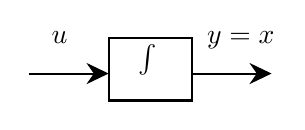
\begin{tikzpicture}[x=0.75pt,y=0.75pt,yscale=-1,xscale=1]
        %uncomment if require: \path (0,300); %set diagram left start at 0, and has height of 300
        
        %Shape: Rectangle [id:dp22292731136066102] 
        \draw   (302,120) -- (342,120) -- (342,150) -- (302,150) -- cycle ;
        %Straight Lines [id:da4024552193434977] 
        \draw    (263.5,137) -- (299,137) ;
        \draw [shift={(302,137)}, rotate = 180] [fill={rgb, 255:red, 0; green, 0; blue, 0 }  ][line width=0.08]  [draw opacity=0] (10.72,-5.15) -- (0,0) -- (10.72,5.15) -- (7.12,0) -- cycle    ;
        %Straight Lines [id:da46675906183124516] 
        \draw    (342.5,137) -- (377.5,137) ;
        \draw [shift={(380.5,137)}, rotate = 180] [fill={rgb, 255:red, 0; green, 0; blue, 0 }  ][line width=0.08]  [draw opacity=0] (10.72,-5.15) -- (0,0) -- (10.72,5.15) -- (7.12,0) -- cycle    ;
        
        \draw (273,115.4) node [anchor=north west][inner sep=0.75pt]    {$u$};
        \draw (348,115.4) node [anchor=north west][inner sep=0.75pt]    {$y=x$};
        \draw (315,121.4) node [anchor=north west][inner sep=0.75pt]  [font=\Large]  {$\int $};

    \end{tikzpicture}

\end{figure}\FloatBarrier

Costruiamo due configurazioni con degli integratori, una in cascata e una in parallelo

\begin{figure}[htpb]\centering
	\tikzset{every picture/.style={line width=0.75pt}} %set default line width to 0.75pt        
	
	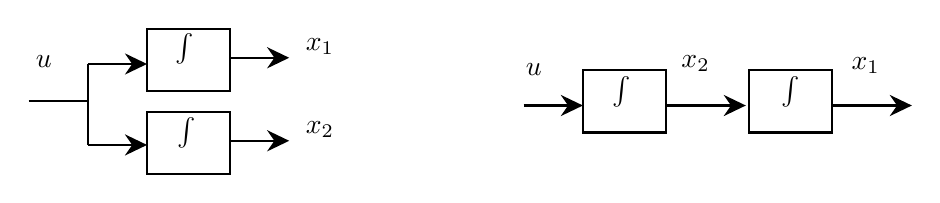
\begin{tikzpicture}[x=0.75pt,y=0.75pt,yscale=-1,xscale=1]
		%uncomment if require: \path (0,110); %set diagram left start at 0, and has height of 110
		
		%Shape: Rectangle [id:dp6579477410290562] 
		\draw   (120,20) -- (160,20) -- (160,50) -- (120,50) -- cycle ;
		%Shape: Rectangle [id:dp8119573056882641] 
		\draw   (120,60) -- (160,60) -- (160,90) -- (120,90) -- cycle ;
		%Shape: Rectangle [id:dp9018179942820435] 
		\draw   (330,40) -- (370,40) -- (370,70) -- (330,70) -- cycle ;
		%Shape: Rectangle [id:dp1323824139504408] 
		\draw   (410,40) -- (450,40) -- (450,70) -- (410,70) -- cycle ;
		\draw    (160,34) -- (185.5,34) ;
		\draw [shift={(188.5,34)}, rotate = 180] [fill={rgb, 255:red, 0; green, 0; blue, 0 }  ][line width=0.08]  [draw opacity=0] (10.72,-5.15) -- (0,0) -- (10.72,5.15) -- (7.12,0) -- cycle    ;
		\draw    (160,74) -- (185.5,74) ;
		\draw [shift={(188.5,74)}, rotate = 180] [fill={rgb, 255:red, 0; green, 0; blue, 0 }  ][line width=0.08]  [draw opacity=0] (10.72,-5.15) -- (0,0) -- (10.72,5.15) -- (7.12,0) -- cycle    ;
		\draw    (301.5,57) -- (327,57) ;
		\draw [shift={(330,57)}, rotate = 180] [fill={rgb, 255:red, 0; green, 0; blue, 0 }  ][line width=0.08]  [draw opacity=0] (10.72,-5.15) -- (0,0) -- (10.72,5.15) -- (7.12,0) -- cycle    ;
		\draw    (370.5,57) -- (405.5,57) ;
		\draw [shift={(408.5,57)}, rotate = 180] [fill={rgb, 255:red, 0; green, 0; blue, 0 }  ][line width=0.08]  [draw opacity=0] (10.72,-5.15) -- (0,0) -- (10.72,5.15) -- (7.12,0) -- cycle    ;
		\draw    (450.5,57) -- (485.5,57) ;
		\draw [shift={(488.5,57)}, rotate = 180] [fill={rgb, 255:red, 0; green, 0; blue, 0 }  ][line width=0.08]  [draw opacity=0] (10.72,-5.15) -- (0,0) -- (10.72,5.15) -- (7.12,0) -- cycle    ;
		\draw    (91.5,37) -- (117,37) ;
		\draw [shift={(120,37)}, rotate = 180] [fill={rgb, 255:red, 0; green, 0; blue, 0 }  ][line width=0.08]  [draw opacity=0] (10.72,-5.15) -- (0,0) -- (10.72,5.15) -- (7.12,0) -- cycle    ;
		\draw    (91.5,76) -- (117,76) ;
		\draw [shift={(120,76)}, rotate = 180] [fill={rgb, 255:red, 0; green, 0; blue, 0 }  ][line width=0.08]  [draw opacity=0] (10.72,-5.15) -- (0,0) -- (10.72,5.15) -- (7.12,0) -- cycle    ;
		\draw    (91.5,37) -- (91.5,76) ;
		\draw    (63,55) -- (91.5,55) ;
		
		\draw (65,31.4) node [anchor=north west][inner sep=0.75pt]    {$u$};
		\draw (195,23.4) node [anchor=north west][inner sep=0.75pt]    {$x_1$};
		\draw (195,63.4) node [anchor=north west][inner sep=0.75pt]    {$x_2$};
		\draw (301,35.4) node [anchor=north west][inner sep=0.75pt]    {$u$};
		\draw (376,31.4) node [anchor=north west][inner sep=0.75pt]    {$x_2$};
		\draw (458,32.4) node [anchor=north west][inner sep=0.75pt]    {$x_1$};

        \draw (132,21) node [anchor=north west][inner sep=0.75pt]  [font=\Large]  {$\int $};
        \draw (133,61.4) node [anchor=north west][inner sep=0.75pt]  [font=\Large]  {$\int $};
        \draw (343,41.4) node [anchor=north west][inner sep=0.75pt]  [font=\Large]  {$\int $};
        \draw (424,41.4) node [anchor=north west][inner sep=0.75pt]  [font=\Large]  {$\int $};
        		
	\end{tikzpicture}
\end{figure}\FloatBarrier

\begin{itemize}
	\item parallelo:\begin{equation*}
	      \begin{array}{ c }
	      	\dot{x}_1 =u \\
	      	\dot{x}_2 =u 
	      \end{array} \ \ \ \ A=\begin{bmatrix}
	      \textcolor[rgb]{0.61,0.61,0.61}{0} & 0\\
	      0 & \textcolor[rgb]{0.61,0.61,0.61}{0}
	\end{bmatrix}
	\end{equation*}
	\item cascata\begin{equation*}
	      \begin{array}{ c }
	      	\dot{x}_1 =x_2 \\
	      	\dot{x}_2 =u   
	      \end{array} \ \ \ \ A=\begin{bmatrix}
	      \textcolor[rgb]{0.61,0.61,0.61}{0} & 1\\
	      0 & \textcolor[rgb]{0.61,0.61,0.61}{0}
	\end{bmatrix}
	\end{equation*}
\end{itemize}

In entrambi i casi gli autovalori sono $\lambda _1 =\lambda _2 =0$ con molteplicità algebrica $a=2$. Per capire in che situazioni siamo studiamo quanti autovettori abbiamo tali che $Ax=\lambda x$ oppure guardiamo il polinomio minimo. $\Delta _A\left(\lambda \right) =\lambda ^2$ in entrambi. Il polinomio minimo può essere, tentandoli tutti, $\psi _A\left(\lambda \right) =\Delta _A\left(\lambda \right) =\lambda ^2$ oppure $\psi _A\left(\lambda \right) =\lambda $. Il polinomio minimo è quello che si annulla in $A$.
\begin{itemize}
	\item parallelo: se $\psi _A\left(\lambda \right) =\lambda $, vediamo se valutato in $A$ si annulla. $\psi _A\left(A\right) =A=0$. Il polinomio minimo è $\lambda $, $b_1 =1$ allora abbiamo \textit{semplice stabilità}.
	\item cascata: se $\psi _A\left(\lambda \right) =\lambda $, vediamo se valutato in $A$ si annulla. $\psi _A\left(A\right) =\begin{bmatrix}
	      0 & 1\\
	      0 & 0
	\end{bmatrix} \neq 0$. Non è il polinomio minimo, allora $b_1 =2$ e abbiamo \textit{instabilità}.
\end{itemize}

\section{Riassunto della stabilità a tempo discreto}

\boxedText{
	Sia $x\left(t+1\right) =Ax\left(t\right)$, allora
	\begin{itemize}
		\item $\left| \lambda _i\right| < 1\ \forall i\iff A$ asint. stabile
		\item $\exists i:\left| \lambda _i\right|  >1\implies A$ instabile (instabilità forte)
		\item $\left| \lambda _i\right| \leq 1\ \forall i,\exists i:\left| \lambda _i\right| =1$
		      \begin{itemize}
		      	\item se $b_i =1\ \left(a_i =n_i\right) \ \forall i\ \left| \lambda _i\right| =1$, cioè quelli critici sono regolari, $\iff A$ sempl. stabile
		      	\item se $b_i  >1\ \left(a_i \neq n_i\right)$ per almeno un $i:\left| \lambda _i\right| =1\implies A$ instabile (debolmente)
		      \end{itemize}
	\end{itemize}
	
	Sono presenti oscillazioni se si verifica almeno una delle due condizioni
	\begin{itemize}
		\item $\exists \lambda _i \in \mathbb{R} ,\lambda _i < 0$
		\item $\exists \lambda _i$ complessi coniugati
	\end{itemize}
}

\section{Sistemi discreti: sistemi a memoria finita}

Consideriamo $x_L\left(t\right) =A^t x\left(0\right)$. Un sistema discreto si dice \textbf{a memoria finita} se $\exists \overline{t}  >0:x_L\left(\overline{t}\right) =0\ \forall x\left(0\right)$, ossia stiamo chiedendo che $A^t$ diventi $0$ in un tempo finito, ossia $A$ è nilpotente $\left(A^{\overline{t}} =0\right)$, ossia tutti gli autovalori sono nulli $\lambda _i =0\ \forall i$.

\textit{In tal caso il tempo di risposta è sempre }$\leq n$\textit{, dato che }$A^n =0$\textit{.}

\section{Test di stabilità}

Un modo furbo per vedere se è stabile.

\subsection{Test della traccia}

\begin{rem}
	Data una qualunque matrice quadrata $A$, la traccia, che per definizione è la somma degli elementi sulla diagonale, è uguale al prodotto degli autovalori
	\begin{equation*}
		\tr A=\sum\limits ^n_{i=1} a_{ii} =\sum\limits ^n_{i=1} \lambda _i
	\end{equation*}
\end{rem}

Consideriamo i sistemi a \textit{tempo continuo} $\dot{x} =Ax$.
\begin{itemize}
	\item Se $\tr A >0$, ovvero $\left(\lambda _1 +\cdots +\lambda _n  >0\right)$, allora esiste almeno un autovalore positivo $\implies A$ instabile.
	\item Se $\tr A=0\implies A$ non è asintoticamente stabile.
	\item Se $\tr A< 0$ non possiamo dedurre niente.
\end{itemize}

Consideriamo i sistemi a \textit{tempo discreto} $x\left(t+1\right) =Ax\left(t\right)$.
\begin{itemize}
	\item Se $\left| \tr A\right|  >n$, allora almeno uno di loro è maggiore di $1$ in modulo $\implies A$ instabile.
	\item Se $\left| \tr A\right| =n\implies A$ non è asintoticamente stabile.
	\item Se $\left| \tr A\right| < n$ non possiamo dedurre niente.
\end{itemize}

\subsection{Test della traccia e del determinante}

Lo si usa nel caso $n=2$.

Consideriamo i sistemi a \textit{tempo continuo} $\dot{x} =Ax$.
\begin{equation*}
	A=\begin{bmatrix}
	a_{11} & a_{12}\\
	a_{21} & a_{22}
	\end{bmatrix} \ \ \ \ \tr A=a_{11} +a_{22} \ \ \ \ \det A=a_{11} a_{22} -a_{12} a_{21}
\end{equation*}
Ricordiamo che la traccia si può anche vedere come la somma degli autovalori, e il determinante come il prodotto degli autovalori. Allora il polinomio caratteristico di $A$ vale
\begin{equation*}
	\begin{aligned}
		\Delta _A\left(\lambda \right) & =\det\left(\lambda I-A\right)                                                   \\
		                               & =\left(\lambda -\lambda _1\right)\left(\lambda -\lambda _2\right)               \\
		                               & =\lambda ^2 -\left(\lambda _1 +\lambda _2\right) \lambda +\lambda _1 \lambda _2 \\
		                               & =\lambda ^2 -\tr A\ \lambda +\det A                                             
	\end{aligned}
\end{equation*}
Si vede quindi che
\begin{itemize}
	\item $A$ è asint. stabile se e solo se stanno entrambi a sinistra dell'asse immaginario, quindi $\tr A< 0$ e $\det A >0$ per assicurarsi che abbiano lo stesso segno
	\item $A$ è instabile se e solo se $\det A< 0$, in tal caso si avrebbe un autovalore strettamente positivo e uno strettamente negativo
	\item $A$ è sempl. stabile se e solo se (non ci sono problemi di regolarità essendo $n=2$) $\det A=0,\tr A< 0$, cioè uno è nullo e l'altro è negativo
\end{itemize}

Consideriamo i sistemi a \textit{tempo discreto} $x\left(t+1\right) =Ax\left(t\right)$.

Non lo dimostriamo perché è rognoso ma si verifica che
\begin{equation*}
	A\ \text{asint. stabile} \ \ \iff \ \ \begin{cases}
	\left| \tr A\right| < 1+\det A\\
	\left| \det A\right| < 1
	\end{cases}
\end{equation*}

\subsection{Test dei coefficienti del polinomio caratteristico}

Si tratta del caso a \textit{tempo continuo} con $n\geq 2$. Se il polinomio caratteristico di $A$ vale
\begin{equation*}
	\Delta _A\left(\lambda \right) =\lambda ^n +\alpha _1 \lambda ^{n-1} +\cdots +\alpha 
\end{equation*}
si può dire che
\begin{equation*}
	\boxed{\text{se} \ A\ \text{è asint. stabile} \ \implies \alpha _i  >0\ \forall i}
\end{equation*}
La coimplicazione vale solo per $n=2$. La dimostrazione è la seguente:
\begin{equation*}
	\begin{aligned}
		\Delta _A\left(\lambda \right) & =\left(\lambda -\lambda _1\right) \cdots \left(\lambda -\lambda _n\right)                                                                                                                                                              \\
		                               & =\lambda ^n +\lambda ^{n-1}\left(\lambda _1 \lambda _2 +\lambda _1 \lambda _3 +\dotsc \right) +\lambda ^{n-2}\left(\lambda _1 \lambda _2 \lambda _3 +\dotsc \right) +\cdots +\left(-1\right)^n \lambda _1 \lambda _2 \dotsc \lambda _n 
	\end{aligned}
\end{equation*}
Se tutti i $\lambda $ sono negativi ($A$ asint. stabile) il loro prodotto è positivo se sono in numero pari, negativo se sono dispari, ma in tal caso c'è $-1$. I prodotti a coppie, i prodotti a terne, e tutti gli altri, danno luogo a coefficienti positivi. Non vale il contrario in generale, ma solo per $n=2$. \textit{È un test rapido per escludere l'asint. stabilità.} Ad esempio, se almeno un coefficiente di $\Delta _A\left(\lambda \right)$ fosse nullo o negativo, possiamo escludere l'asint. stabilità subito.

\section{Test di Hurwitz (sistemi a tempo continuo)}

Consideriamo $\dot{x} =Ax$ e il polinomio caratteristico
\begin{equation*}
	\Delta _A\left(\lambda \right) =\lambda ^n +\alpha _1 \lambda ^{n-1} +\cdots +\alpha _n
\end{equation*}
Costruiamo la matrice $H\in \mathbb{R}^{n\times n}$, ciascuna riga comincia con i coefficienti dispari, e prosegue in ordine descrescente coi rimanenti, poi un $1$ e infine $0$ fino in fondo. Riempiamo righe fino alla fine. Se arriviamo a riempire tutti gli $\alpha _i$ si pongono $\alpha _i =0,\forall i >n$.
\begin{equation*}
	H=\begin{bmatrix}
	\alpha _1 & 1 & 0 & 0 & 0 & \dotsc  & \\
	\alpha _3 & \alpha _2 & \alpha _1 & 1 & 0 & \dotsc  & \\
	\alpha _5 & \alpha _4 & \alpha _3 & \alpha _2 & \alpha _1 & 1 & 0\\
	\vdots  &  &  &  &  &  & \\
	&  &  &  &  &  & \\
	&  &  &  &  &  & \\
	&  &  &  &  &  & 
	\end{bmatrix} \in \mathbb{R}^{n\times n}
\end{equation*}
Se consideriamo le sottomatrici appoggiate all'angolo Nord-Ovest, di dimensione crescente $D_1 ,D_2 ,\dotsc ,D_n =H$ il criterio di Hurwitz afferma che
\begin{equation*}
	\boxed{A\ \text{asint. stabile} \ \ \iff \ \ \det D_i  >0\ \forall i=1,\dotsc ,n}
\end{equation*}
Non sappiamo nulla su dinamiche oscillatorie, tempi di risposta ecc. Vediamo anche nello specifico due casi:
\begin{itemize}
	\item $n=2$, il polinomio caratteristico è $\Delta _A\left(\lambda \right) =\lambda ^2 +\alpha _1 \lambda +\alpha _2$, la matrice $H$ è quindi\begin{equation*}
	      H=\begin{bmatrix}
	      \alpha _1 & 1\\
	      0 & \alpha _2
	\end{bmatrix}
	\end{equation*}
	
	di conseguenza per il criterio di Hurwitz\begin{equation*}
	A\ \text{asint. stabile} \ \ \iff \ \ \alpha _1  >0,\alpha _2  >0
	\end{equation*}
	\item $n=3$, il polinomio caratteristico è $\Delta _A\left(\lambda \right) =\lambda ^3 +\alpha _1 \lambda ^2 +\alpha _2 \lambda +\alpha _3$, la matrice $H$ è quindi\begin{equation*}
	      H=\begin{bmatrix}
	      \alpha _1 & 1 & 0\\
	      \alpha _3 & \alpha _2 & 1\\
	      0 & 0 & \alpha _3
	\end{bmatrix}
	\end{equation*}
	
	di conseguenza per il criterio di Hurwitz $A$ è asint. stabile se e solo se\begin{equation*}
	\begin{cases}
		\alpha _1  >0                                                              \\
		\alpha _2 \alpha _1  >\alpha _3 \ \left(\text{cioè} \ \det D_2  >0\right) \\
		\alpha _3\left(\det D_2\right)  >0                                         
	\end{cases} \ \ \iff \ \ \begin{cases}
	\alpha _i  >0,\forall i\\
	\alpha _2 \alpha _1  >\alpha _3
	\end{cases}
	\end{equation*}
\end{itemize}

\section{Criterio righe/colonne}

Consideriamo due tipi di matrici, rispettivamente per i sistemi a tempo continuo e discreto:
\begin{itemize}
	\item t. continuo: \textbf{matrici di Metzler} (o matrici essenzialmente non negative), sono tali che $a_{ij} \geq 0,\forall i\neq j$
	\item t. discreto: \textbf{matrici non negative}, sono tali che $a_{ij} \geq 0$
\end{itemize}

Se sussistono queste cose, vale la seguente proprietà: \textit{se tutte le componenti del vettore di stato }$x_i(t)$\textit{ sono non negative allo stato iniziale, allora si mantengono tali} (\textbf{sistemi positivi}); questa proprietà è molto comune, ad esempio nei sistemi compartimentali. Vediamo un'altra interessante proprietà di questi sistemi, parte del lavoro sviluppato da Frobenius e Perron.

Ricordiamo che per una generica matrice vale:
\begin{itemize}
	\item t. continuo: un sistema è asint. stabile se e solo se $\Re(\lambda _D) < 0$
	\item t. discreto: un sistema è asint. stabile se e solo se $| \lambda _D| < 1$
\end{itemize}

Nel caso di queste matrici, l'autovalore dominante soddisfa le proprietà:
\begin{itemize}
	\item t. continuo: $\lambda _D$ è \textbf{reale.}
	\item t. discreto: $\exists \lambda _D$ è \textbf{reale non negativo.}
\end{itemize}

Rimanendo nel caso di queste matrici, enunciamo il \textbf{criterio righe/colonne}. La seguente cosa vale per tutte le matrici, sia derivanti da sistemi continui che discreti, poi starà a noi discutere $\lambda _D$ in base al tipo di sistema. Scriviamo la matrice $A$, le somme di riga e le somme di colonna:
\begin{equation*}
	\begin{array}{ r l }
		A=\begin{bmatrix}
		a_{11} & a_{12} & \dotsc & a_{1n} \\
		a_{21} & a_{22} & \dotsc & a_{2n} \\
		\vdots & \vdots & \ddots & \vdots \\
		a_{n1} & a_{n2} & \dotsc & a_{nn} 
		\end{bmatrix} & \begin{array}{ c }
		r_1\\
		r_2\\
		\vdots \\
		r_n
	\end{array}\\
	& \\
	\begin{array}{ c c c c }
		c_{1\ } & c_{2\ } & \dotsc & c_{n\ } 
	\end{array} & 
	\end{array}
\end{equation*}
Allora valgono le seguenti $4$ disuguaglianze
\begin{equation*}
	\boxed{
		\begin{array}{{>{\displaystyle}l}}
			\min r_i \leq \lambda _D \leq \max r_i \\
			\min c_i \leq \lambda _D \leq \max c_i 
		\end{array}
	}
\end{equation*}

\chapter{Sistemi aggregati}

\begin{figure}[htpb]\centering
	\tikzset{every picture/.style={line width=0.75pt}} %set default line width to 0.75pt        
	
	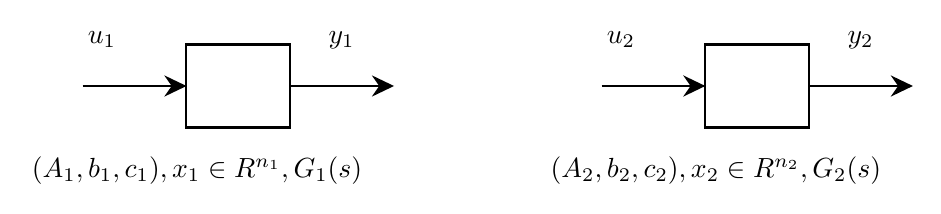
\begin{tikzpicture}[x=0.75pt,y=0.75pt,yscale=-1,xscale=1]
		%uncomment if require: \path (0,111); %set diagram left start at 0, and has height of 111
		
		%Shape: Rectangle [id:dp5639908995287914] 
		\draw   (150,20) -- (200,20) -- (200,60) -- (150,60) -- cycle ;
		\draw    (100,40) -- (147,40) ;
		\draw [shift={(150,40)}, rotate = 180] [fill={rgb, 255:red, 0; green, 0; blue, 0 }  ][line width=0.08]  [draw opacity=0] (10.72,-5.15) -- (0,0) -- (10.72,5.15) -- (7.12,0) -- cycle    ;
		\draw    (200,40) -- (247,40) ;
		\draw [shift={(250,40)}, rotate = 180] [fill={rgb, 255:red, 0; green, 0; blue, 0 }  ][line width=0.08]  [draw opacity=0] (10.72,-5.15) -- (0,0) -- (10.72,5.15) -- (7.12,0) -- cycle    ;
		%Shape: Rectangle [id:dp5024964536638126] 
		\draw   (400,20) -- (450,20) -- (450,60) -- (400,60) -- cycle ;
		\draw    (350,40) -- (397,40) ;
		\draw [shift={(400,40)}, rotate = 180] [fill={rgb, 255:red, 0; green, 0; blue, 0 }  ][line width=0.08]  [draw opacity=0] (10.72,-5.15) -- (0,0) -- (10.72,5.15) -- (7.12,0) -- cycle    ;
		\draw    (450,40) -- (497,40) ;
		\draw [shift={(500,40)}, rotate = 180] [fill={rgb, 255:red, 0; green, 0; blue, 0 }  ][line width=0.08]  [draw opacity=0] (10.72,-5.15) -- (0,0) -- (10.72,5.15) -- (7.12,0) -- cycle    ;
		
		\draw (101,12.4) node [anchor=north west][inner sep=0.75pt]    {$u_1$};
		\draw (217,12.4) node [anchor=north west][inner sep=0.75pt]    {$y_1$};
		\draw (74,72.4) node [anchor=north west][inner sep=0.75pt]    {$(A_1 ,b_1 ,c_1) ,x_1 \in \mathbb{R}^{n_1} ,G_1(s)$};
		\draw (351,12.4) node [anchor=north west][inner sep=0.75pt]    {$u_2$};
		\draw (467,12.4) node [anchor=north west][inner sep=0.75pt]    {$y_2$};
		\draw (324,72.4) node [anchor=north west][inner sep=0.75pt]    {$(A_2 ,b_2 ,c_2) ,x_2 \in \mathbb{R}^{n_2} ,G_2(s)$};
		
		
	\end{tikzpicture}
\end{figure}\FloatBarrier

\section{Cascata}

In questo caso $u_2 =y_1 =c_1 x_1$ e $x=\begin{bmatrix}
x_1\\
x_2
\end{bmatrix} \in \mathbb{R}^{n_1 +n_2}$. Quindi complessivamente lo stato
\begin{equation*}
	\begin{aligned}
		\dot{x} =\begin{bmatrix}
		\dot{x}_1\\
		\dot{x}_2
		\end{bmatrix} & =\begin{bmatrix}             
		A_1 x_1 +b_1 u_1\\
		A_2 x_2 +b_2 u_2
		\end{bmatrix}\\
		              & =\begin{bmatrix}             
		A_1 x_1 +b_1 u_1\\
		A_2 x_2 +b_2 c_1 x_1
		\end{bmatrix}\\
		              & =\underbrace{\begin{bmatrix} 
		A_1           & 0                            \\
		b_2 c_1       & A_2                          
		\end{bmatrix}
		}_{\tilde{A}}\begin{bmatrix}
		x_1\\
		x_2
		\end{bmatrix} +\underbrace{\begin{bmatrix}
		b_1\\
		0
		\end{bmatrix}
		}_{\tilde{b}} u
	\end{aligned}
\end{equation*}
mentre l'uscita
\begin{equation*}
	y=y_2 =c_2 x_2 =\underbrace{\begin{bmatrix}
		0 & c_2
		\end{bmatrix}
		}_{\tilde{c}}\begin{bmatrix}
	x_1\\
	x_2
	\end{bmatrix}
\end{equation*}
Osserviamo che $\tilde{A}$ è triangolare a blocchi
\begin{equation*}
	\boxed{\sigma \left(\tilde{A}\right) =\sigma \left(A_1\right) \cup \sigma \left(A_2\right)}
\end{equation*}
\textbf{Quindi }$\tilde{A}$\textbf{ è asint. stabile se e solo se }$A_1 ,A_2$\textbf{ sono asint. stabili, mentre }$\tilde{A}$\textbf{ è fortemente instabile se e solo se almeno uno tra }$A_1 ,A_2$\textbf{ è fortemente instabile.}

Per quanto riguarda le funzioni di trasferimento vale
\begin{equation*}
	y=G_2 u_2 =G_2 y_1 =G_2 G_1 u_1 \implies \boxed{G\left(s\right) =G_1\left(s\right) G_2\left(s\right)}
\end{equation*}

\section{Parallelo}

In questo caso $u_1 =u_2 =u$. Si verifica
\begin{equation*}
	\tilde{A} =\begin{bmatrix}
	A_1 & 0\\
	0 & A_2
	\end{bmatrix}
\end{equation*}
Il discorso sulla stabilità è uguale. Per la funzione di trasferimento vale
\begin{equation*}
	y=y_1 +y_2 =G_1 u_1 +G_2 u_2 =\left(G_1 +G_2\right) u\implies \boxed{G\left(s\right) =G_1\left(s\right) +G_2\left(s\right)}
\end{equation*}

\section{Retroazione}

\begin{figure}[htpb]\centering
	\tikzset{every picture/.style={line width=0.75pt}} %set default line width to 0.75pt        
	
	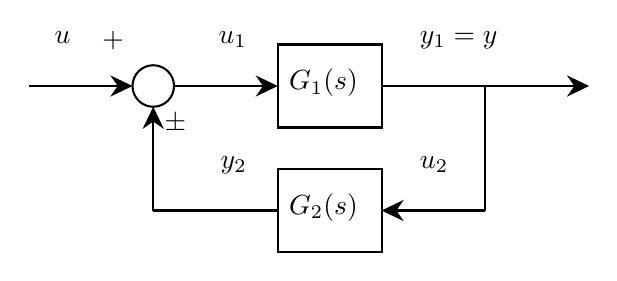
\begin{tikzpicture}[x=0.75pt,y=0.75pt,yscale=-1,xscale=1]
		%uncomment if require: \path (0,129); %set diagram left start at 0, and has height of 129
		
		%Shape: Rectangle [id:dp538055796397179] 
		\draw   (280,20) -- (330,20) -- (330,60) -- (280,60) -- cycle ;
		\draw    (230,40) -- (277,40) ;
		\draw [shift={(280,40)}, rotate = 180] [fill={rgb, 255:red, 0; green, 0; blue, 0 }  ][line width=0.08]  [draw opacity=0] (10.72,-5.15) -- (0,0) -- (10.72,5.15) -- (7.12,0) -- cycle    ;
		\draw    (330,40) -- (427,40) ;
		\draw [shift={(430,40)}, rotate = 180] [fill={rgb, 255:red, 0; green, 0; blue, 0 }  ][line width=0.08]  [draw opacity=0] (10.72,-5.15) -- (0,0) -- (10.72,5.15) -- (7.12,0) -- cycle    ;
		%Shape: Rectangle [id:dp5156139345780957] 
		\draw   (280,80) -- (330,80) -- (330,120) -- (280,120) -- cycle ;
		\draw    (220,100) -- (220,53) ;
		\draw [shift={(220,50)}, rotate = 450] [fill={rgb, 255:red, 0; green, 0; blue, 0 }  ][line width=0.08]  [draw opacity=0] (10.72,-5.15) -- (0,0) -- (10.72,5.15) -- (7.12,0) -- cycle    ;
		\draw    (380,100) -- (333,100) ;
		\draw [shift={(330,100)}, rotate = 360] [fill={rgb, 255:red, 0; green, 0; blue, 0 }  ][line width=0.08]  [draw opacity=0] (10.72,-5.15) -- (0,0) -- (10.72,5.15) -- (7.12,0) -- cycle    ;
		%Shape: Circle [id:dp6988631785539583] 
		\draw   (210,40) .. controls (210,34.48) and (214.48,30) .. (220,30) .. controls (225.52,30) and (230,34.48) .. (230,40) .. controls (230,45.52) and (225.52,50) .. (220,50) .. controls (214.48,50) and (210,45.52) .. (210,40) -- cycle ;
		\draw    (160,40) -- (207,40) ;
		\draw [shift={(210,40)}, rotate = 180] [fill={rgb, 255:red, 0; green, 0; blue, 0 }  ][line width=0.08]  [draw opacity=0] (10.72,-5.15) -- (0,0) -- (10.72,5.15) -- (7.12,0) -- cycle    ;
		\draw    (220,100) -- (280,100) ;
		\draw    (380,40) -- (380,100) ;
		
		\draw (250,12.4) node [anchor=north west][inner sep=0.75pt]    {$u_1$};
		\draw (347,12.4) node [anchor=north west][inner sep=0.75pt]    {$y_1 =y$};
		\draw (251,72.4) node [anchor=north west][inner sep=0.75pt]    {$y_2$};
		\draw (347,72.4) node [anchor=north west][inner sep=0.75pt]    {$u_2$};
		\draw (171,12.4) node [anchor=north west][inner sep=0.75pt]    {$u$};
		\draw (194,12.4) node [anchor=north west][inner sep=0.75pt]    {$+$};
		\draw (224,52.4) node [anchor=north west][inner sep=0.75pt]    {$\pm $};
		\draw (284,30.4) node [anchor=north west][inner sep=0.75pt]    {$G_1(s)$};
		\draw (284,90.4) node [anchor=north west][inner sep=0.75pt]    {$G_2(s)$};
		
		
	\end{tikzpicture}
\end{figure}\FloatBarrier

In questo caso $y=y_1 =u_2$ e $u_1 =u\pm y_2$. Quindi
\begin{equation*}
	\begin{aligned}
		\dot{x} =\begin{bmatrix}
		\dot{x}_1\\
		\dot{x}_2
		\end{bmatrix} & =\begin{bmatrix}             
		A_1 x_1 +b_1 u_1\\
		A_2 x_2 +b_2 u_2
		\end{bmatrix}\\
		              & =\begin{bmatrix}             
		\ \ \ A_1 x_1 +b_1(u\pm y_2)\\
		A_2 x_2 +b_2 y_1
		\end{bmatrix}\\
		              & =\begin{bmatrix}             
		\ \ \ A_1 x_1 +b_1 u\pm b_1 c_2 x_2\\
		A_2 x_2 +b_2 c_1 x_1
		\end{bmatrix}\\
		              & =\underbrace{\begin{bmatrix} 
		A_1           & \pm b_1 c_2                  \\
		b_2 c_1       & A_2                          
		\end{bmatrix}
		}_{\tilde{A}}\begin{bmatrix}
		x_1\\
		x_2
		\end{bmatrix} +\underbrace{\begin{bmatrix}
		b_1\\
		0
		\end{bmatrix}
		}_{\tilde{b}} u
	\end{aligned}
\end{equation*}
mentre l'uscita
\begin{equation*}
	y=y_1 =c_1 x_1 =\underbrace{\begin{bmatrix}
		c_1 & 0
		\end{bmatrix}
		}_{\tilde{c}}\begin{bmatrix}
	x_1\\
	x_2
	\end{bmatrix}
\end{equation*}
La matrice $\tilde{A}$ non ha strutture particolari. \textbf{Le matrici }$A_1 ,A_2$\textbf{ non dicono nulla a priori sulla stabilità dell'aggregato.} Bisogna studiare caso per caso.

Per la funzione di trasferimento vale
\begin{equation*}
	\begin{aligned}
		y=y_1 & =G_1\left(u\pm y_2\right) \\
		      & =G_1 u\pm G_1 y_2         \\
		      & =G_1 u\pm G_1 G_2 u_2     \\
		      & =G_1 u\pm G_1 G_2 y       
	\end{aligned}
\end{equation*}
Possiamo raccogliere la $y$
\begin{equation*}
	y\left(1\mp G_1 G_2\right) =G_1 u\implies y=\frac{G_1}{1\mp G_1 G_2} u\implies \boxed{G\left(s\right) =\frac{G_1\left(s\right)}{1\mp G_1\left(s\right) G_2\left(s\right)}}
\end{equation*}
$G_1(s)G_2(s)=:L(s)$ è detta \textbf{funzione di trasferimento d'anello}, in quanto attraverso questa stiamo facendo un giro completo dell'anello che parte e si conclude nel nodo sommatore.

\chapter{Studio delle traiettorie}

Studieremo le traiettorie per i sistemi a t. continuo e con $n=2$. Il sistema che studiamo è
\begin{equation*}
	\dot{x} =Ax+bu
\end{equation*}
ma possiamo semplificare il nostro studio supponendo $u\left(t\right) =\overline{u} =0,\ \forall t\geq 0$. Non perdiamo generalità in quanto a meno di un cambio di coordinate possiamo traslare il movimento. Infatti se $\overline{u} \neq 0$ e $\overline{x}$ è il nostro equilibrio, si ha
\begin{equation*}
	\begin{aligned}
		z=x-\overline{x} \implies \dot{z} & =\dot{x}                                           \\
		                                     & =Ax+b\overline{u}                                  \\
		                                     & =A\left(z+\overline{x}\right) +b\overline{u}       \\
		                                     & =Az+\underbrace{A\overline{x} +b\overline{u}}_{=0} 
	\end{aligned}
\end{equation*}
infatti $\overline{x}$ è equilibrio. Quindi possiamo studiare semplicemente
\begin{equation*}
	\dot{x} =Ax
\end{equation*}
Matricialmente abbiamo
\begin{equation*}
	A=\begin{bmatrix}
	a_{11} & a_{12}\\
	a_{21} & a_{22}
	\end{bmatrix} \ \ \ \ \sigma \left(A\right) =\left\{\lambda _1 ,\lambda _2\right\}
\end{equation*}
Consideriamo l'\textbf{equazione agli autovettori}
\begin{equation*}
	\boxed{Ax=\lambda _i x}
\end{equation*}
Se $x$ è l'autovettore relativo all'autovalore $\lambda _i$, allora anche $\alpha x$ lo è $\left(\alpha \in \mathbb{R} ,\alpha \neq 0\right)$. Inoltre, sempre se $x$ è l'autovettore, l'equazione agli autovettori si può pensare come
\begin{equation*}
	\dot{x} =Ax=\lambda _i x\ \ \iff \ \ \begin{bmatrix}
	\dot{x}_1\\
	\dot{x}_2
	\end{bmatrix} =\begin{bmatrix}
	\lambda _i x_1\\
	\lambda _i x_2
	\end{bmatrix} \ \ \iff \ \ \begin{array}{ c }
	x_1\left(t\right) =e^{\lambda _i t} x_1\left(0\right)\\
	x_2\left(t\right) =e^{\lambda _i t} x_2\left(0\right)
	\end{array}
\end{equation*}
deduciamo che \textbf{gli autovettori sono gli unici luoghi di traiettorie rettilinee}: se $\lambda $ è negativo, è percorso verso $0$, se è positivo è percorso verso $+\infty $, se è nullo rimane costante. Partendo da un qualunque altro punto si ha combinazione lineare di tutti i modi. Analizziamo una serie di casi per capire cosa succede, sempre nel caso $\dot{x} =Ax$.
\begin{itemize}
	\item \textbf{Autovalori reali negativi.} Le traiettorie tendono all'equilibrio, $0$ in questo caso, tangenti all'autovalore dominante, ovvero quello più lento, quello più a destra possibile. Si dice \textit{nodo stabile}.
	      
	      \begin{figure}[htpb]\centering
	      	\tikzset{every picture/.style={line width=0.75pt}} %set default line width to 0.75pt        
	      	
	      	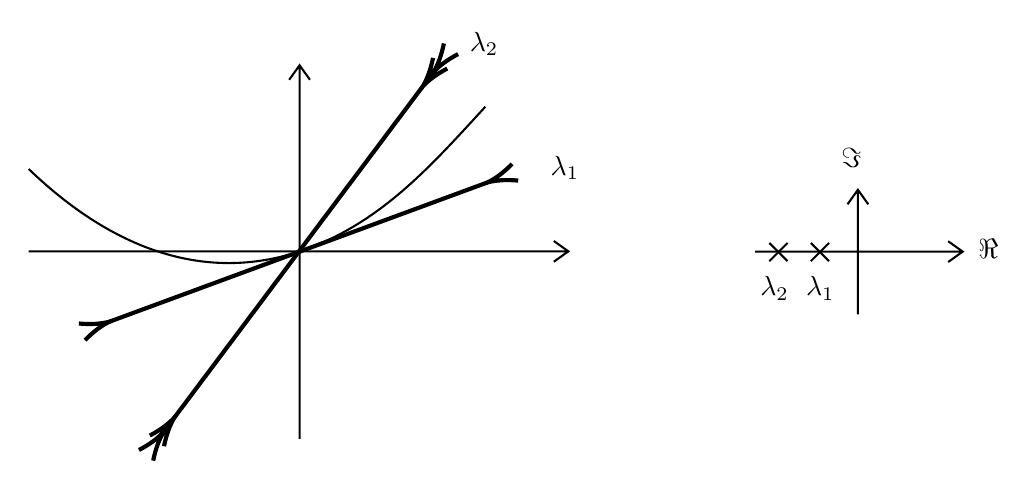
\begin{tikzpicture}[x=0.75pt,y=0.75pt,yscale=-1,xscale=1]
	      		%uncomment if require: \path (0,230); %set diagram left start at 0, and has height of 230
	      		
	      		%Shape: Axis 2D [id:dp6875582348915052] 
	      		\draw  (20,119.67) -- (280,119.67)(150.5,30) -- (150.5,210) (273,114.67) -- (280,119.67) -- (273,124.67) (145.5,37) -- (150.5,30) -- (155.5,37)  ;
	      		\draw [line width=1.5]    (209.7,40.4) -- (90.3,199.6) ;
	      		\draw [shift={(90.3,199.6)}, rotate = 126.87] [color={rgb, 255:red, 0; green, 0; blue, 0 }  ][line width=1.5]    (22.93,-4.28) .. controls (17.76,-1.82) and (13.02,-0.39) .. (8.72,0) .. controls (13.02,0.39) and (17.76,1.82) .. (22.93,4.28)(14.21,-4.28) .. controls (9.04,-1.82) and (4.3,-0.39) .. (0,0) .. controls (4.3,0.39) and (9.04,1.82) .. (14.21,4.28)   ;
	      		\draw [shift={(209.7,40.4)}, rotate = 306.87] [color={rgb, 255:red, 0; green, 0; blue, 0 }  ][line width=1.5]    (22.93,-4.28) .. controls (17.76,-1.82) and (13.02,-0.39) .. (8.72,0) .. controls (13.02,0.39) and (17.76,1.82) .. (22.93,4.28)(14.21,-4.28) .. controls (9.04,-1.82) and (4.3,-0.39) .. (0,0) .. controls (4.3,0.39) and (9.04,1.82) .. (14.21,4.28)   ;
	      		\draw [line width=1.5]    (241.02,86.47) -- (58.98,153.53) ;
	      		\draw [shift={(58.98,153.53)}, rotate = 159.78] [color={rgb, 255:red, 0; green, 0; blue, 0 }  ][line width=1.5]    (14.21,-4.28) .. controls (9.04,-1.82) and (4.3,-0.39) .. (0,0) .. controls (4.3,0.39) and (9.04,1.82) .. (14.21,4.28)   ;
	      		\draw [shift={(241.02,86.47)}, rotate = 339.78] [color={rgb, 255:red, 0; green, 0; blue, 0 }  ][line width=1.5]    (14.21,-4.28) .. controls (9.04,-1.82) and (4.3,-0.39) .. (0,0) .. controls (4.3,0.39) and (9.04,1.82) .. (14.21,4.28)   ;
	      		%Shape: Axis 2D [id:dp39976626315956043] 
	      		\draw  (370,119.8) -- (470,119.8)(419.5,90) -- (419.5,150) (463,114.8) -- (470,119.8) -- (463,124.8) (414.5,97) -- (419.5,90) -- (424.5,97)  ;
	      		\draw   (376.82,115.61) -- (385.61,124.39)(385.61,115.61) -- (376.82,124.39) ;
	      		\draw   (396.82,115.61) -- (405.61,124.39)(405.61,115.61) -- (396.82,124.39) ;
	      		%Curve Lines [id:da5813584010157853] 
	      		\draw    (20,80) .. controls (66.5,124.67) and (111.5,132.67) .. (150.5,119.67) .. controls (189.5,106.67) and (214.5,77.67) .. (240,50) ;
	      		
	      		\draw (270,72.4) node [anchor=north west][inner sep=0.75pt]    {$\lambda _1$};
	      		\draw (231,12.4) node [anchor=north west][inner sep=0.75pt]    {$\lambda _2$};
	      		\draw (476,112.4) node [anchor=north west][inner sep=0.75pt]    {$\Re$};
	      		\draw (410,68.4) node [anchor=north west][inner sep=0.75pt]    {$\Im$};
	      		\draw (393,130.4) node [anchor=north west][inner sep=0.75pt]    {$\lambda _1$};
	      		\draw (371,130.4) node [anchor=north west][inner sep=0.75pt]    {$\lambda _2$};
	      		
	      		
	      	\end{tikzpicture}
	      \end{figure}\FloatBarrier
	      
	\item \textbf{Autovalori reali, uno negativo e uno positivo.} Si ha divergenza ovunque fuorché lungo l'autovettore relativo all'autovalore negativo. Si dice \textit{sella}.
	      
	      \begin{figure}[htpb]\centering
	      	\tikzset{every picture/.style={line width=0.75pt}} %set default line width to 0.75pt        
	      	
	      	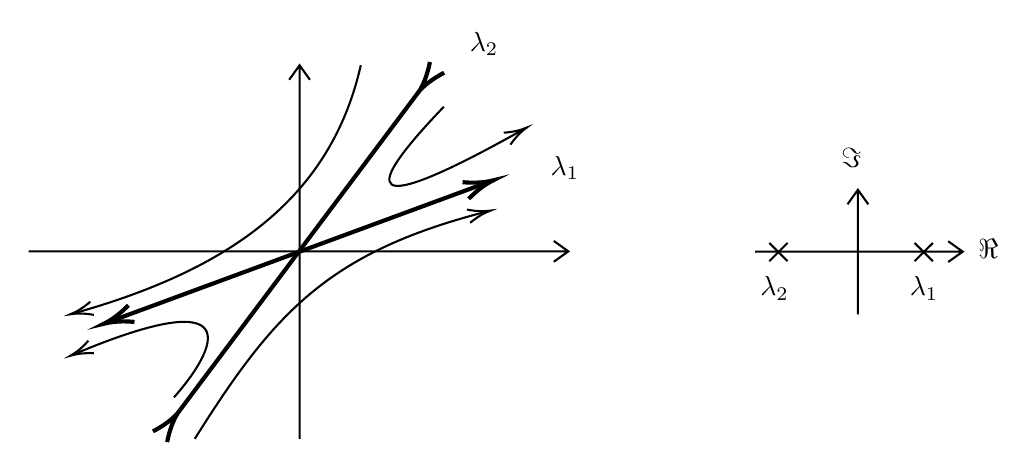
\begin{tikzpicture}[x=0.75pt,y=0.75pt,yscale=-1,xscale=1]
	      		%uncomment if require: \path (0,230); %set diagram left start at 0, and has height of 230
	      		
	      		%Shape: Axis 2D [id:dp8911138419019224] 
	      		\draw  (20,119.67) -- (280,119.67)(150.5,30) -- (150.5,210) (273,114.67) -- (280,119.67) -- (273,124.67) (145.5,37) -- (150.5,30) -- (155.5,37)  ;
	      		\draw [line width=1.5]    (208.2,42.4) -- (91.8,197.6) ;
	      		\draw [shift={(91.8,197.6)}, rotate = 126.87] [color={rgb, 255:red, 0; green, 0; blue, 0 }  ][line width=1.5]    (14.21,-4.28) .. controls (9.04,-1.82) and (4.3,-0.39) .. (0,0) .. controls (4.3,0.39) and (9.04,1.82) .. (14.21,4.28)   ;
	      		\draw [shift={(208.2,42.4)}, rotate = 306.87] [color={rgb, 255:red, 0; green, 0; blue, 0 }  ][line width=1.5]    (14.21,-4.28) .. controls (9.04,-1.82) and (4.3,-0.39) .. (0,0) .. controls (4.3,0.39) and (9.04,1.82) .. (14.21,4.28)   ;
	      		\draw [line width=1.5]    (241.02,86.47) -- (58.98,153.53) ;
	      		\draw [shift={(56.16,154.56)}, rotate = 339.78] [color={rgb, 255:red, 0; green, 0; blue, 0 }  ][line width=1.5]    (14.21,-4.28) .. controls (9.04,-1.82) and (4.3,-0.39) .. (0,0) .. controls (4.3,0.39) and (9.04,1.82) .. (14.21,4.28)   ;
	      		\draw [shift={(243.84,85.44)}, rotate = 159.78] [color={rgb, 255:red, 0; green, 0; blue, 0 }  ][line width=1.5]    (14.21,-4.28) .. controls (9.04,-1.82) and (4.3,-0.39) .. (0,0) .. controls (4.3,0.39) and (9.04,1.82) .. (14.21,4.28)   ;
	      		%Shape: Axis 2D [id:dp4830817817842632] 
	      		\draw  (370,119.8) -- (470,119.8)(419.5,90) -- (419.5,150) (463,114.8) -- (470,119.8) -- (463,124.8) (414.5,97) -- (419.5,90) -- (424.5,97)  ;
	      		\draw   (376.82,115.61) -- (385.61,124.39)(385.61,115.61) -- (376.82,124.39) ;
	      		\draw   (446.82,115.61) -- (455.61,124.39)(455.61,115.61) -- (446.82,124.39) ;
	      		%Curve Lines [id:da48448025642571535] 
	      		\draw    (42.32,149.36) .. controls (118.46,127.97) and (165.65,93.04) .. (180,30) ;
	      		\draw [shift={(40,150)}, rotate = 344.61] [color={rgb, 255:red, 0; green, 0; blue, 0 }  ][line width=0.75]    (10.93,-3.29) .. controls (6.95,-1.4) and (3.31,-0.3) .. (0,0) .. controls (3.31,0.3) and (6.95,1.4) .. (10.93,3.29)   ;
	      		%Curve Lines [id:da7291927916904639] 
	      		\draw    (240.19,100.62) .. controls (164.06,120.31) and (138.12,149.29) .. (100,210) ;
	      		\draw [shift={(242.51,100.03)}, rotate = 165.81] [color={rgb, 255:red, 0; green, 0; blue, 0 }  ][line width=0.75]    (10.93,-3.29) .. controls (6.95,-1.4) and (3.31,-0.3) .. (0,0) .. controls (3.31,0.3) and (6.95,1.4) .. (10.93,3.29)   ;
	      		%Curve Lines [id:da7821735169413289] 
	      		\draw    (90,190) .. controls (111.39,165.79) and (125.36,133.99) .. (41.28,169.46) ;
	      		\draw [shift={(40,170)}, rotate = 336.98] [color={rgb, 255:red, 0; green, 0; blue, 0 }  ][line width=0.75]    (10.93,-3.29) .. controls (6.95,-1.4) and (3.31,-0.3) .. (0,0) .. controls (3.31,0.3) and (6.95,1.4) .. (10.93,3.29)   ;
	      		%Curve Lines [id:da45885792473728704] 
	      		\draw    (258.16,61.03) .. controls (197.91,94.85) and (169.02,103.14) .. (220,50) ;
	      		\draw [shift={(260,60)}, rotate = 150.59] [color={rgb, 255:red, 0; green, 0; blue, 0 }  ][line width=0.75]    (10.93,-3.29) .. controls (6.95,-1.4) and (3.31,-0.3) .. (0,0) .. controls (3.31,0.3) and (6.95,1.4) .. (10.93,3.29)   ;
	      		
	      		\draw (270,72.4) node [anchor=north west][inner sep=0.75pt]    {$\lambda _1$};
	      		\draw (231,12.4) node [anchor=north west][inner sep=0.75pt]    {$\lambda _2$};
	      		\draw (476,112.4) node [anchor=north west][inner sep=0.75pt]    {$\Re$};
	      		\draw (410,68.4) node [anchor=north west][inner sep=0.75pt]    {$\Im$};
	      		\draw (443,130.4) node [anchor=north west][inner sep=0.75pt]    {$\lambda _1$};
	      		\draw (371,130.4) node [anchor=north west][inner sep=0.75pt]    {$\lambda _2$};
	      		
	      		
	      	\end{tikzpicture}
	      \end{figure}\FloatBarrier
	      
	\item \textbf{Autovalori reali positivi.} C'è divergenza ovunque, tendendo a essere paralleli a quello dominante. Si dice \textit{nodo instabile}.
	      
	      \begin{figure}[htpb]\centering
	      	\tikzset{every picture/.style={line width=0.75pt}} %set default line width to 0.75pt        
	      	
	      	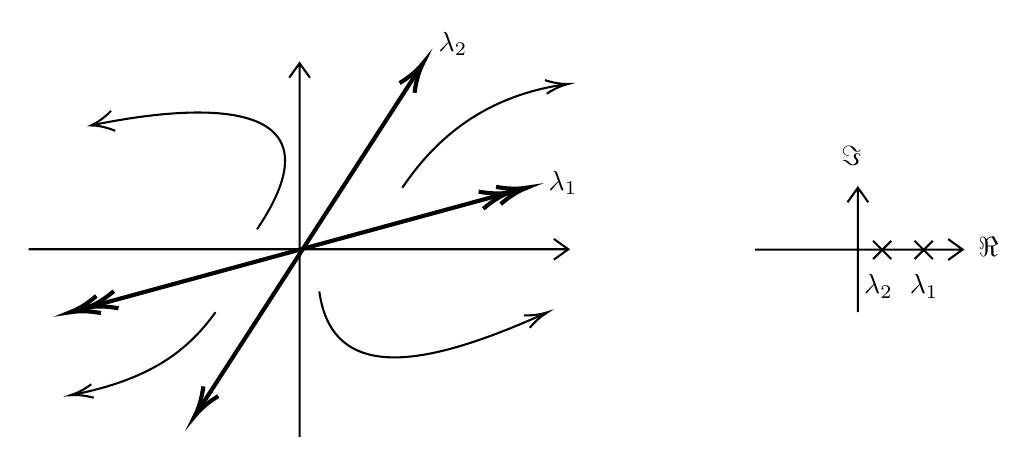
\begin{tikzpicture}[x=0.75pt,y=0.75pt,yscale=-1,xscale=1]
	      		%uncomment if require: \path (0,230); %set diagram left start at 0, and has height of 230
	      		
	      		%Shape: Axis 2D [id:dp618889605882575] 
	      		\draw  (20,119.67) -- (280,119.67)(150.5,30) -- (150.5,210) (273,114.67) -- (280,119.67) -- (273,124.67) (145.5,37) -- (150.5,30) -- (155.5,37)  ;
	      		\draw [line width=1.5]    (208.37,32.52) -- (101.63,197.48) ;
	      		\draw [shift={(100,200)}, rotate = 302.90999999999997] [color={rgb, 255:red, 0; green, 0; blue, 0 }  ][line width=1.5]    (14.21,-4.28) .. controls (9.04,-1.82) and (4.3,-0.39) .. (0,0) .. controls (4.3,0.39) and (9.04,1.82) .. (14.21,4.28)   ;
	      		\draw [shift={(210,30)}, rotate = 122.91] [color={rgb, 255:red, 0; green, 0; blue, 0 }  ][line width=1.5]    (14.21,-4.28) .. controls (9.04,-1.82) and (4.3,-0.39) .. (0,0) .. controls (4.3,0.39) and (9.04,1.82) .. (14.21,4.28)   ;
	      		\draw [line width=1.5]    (260,90) -- (40,150) ;
	      		\draw [shift={(40,150)}, rotate = 344.74] [color={rgb, 255:red, 0; green, 0; blue, 0 }  ][line width=1.5]    (22.93,-4.28) .. controls (17.76,-1.82) and (13.02,-0.39) .. (8.72,0) .. controls (13.02,0.39) and (17.76,1.82) .. (22.93,4.28)(14.21,-4.28) .. controls (9.04,-1.82) and (4.3,-0.39) .. (0,0) .. controls (4.3,0.39) and (9.04,1.82) .. (14.21,4.28)   ;
	      		\draw [shift={(260,90)}, rotate = 164.74] [color={rgb, 255:red, 0; green, 0; blue, 0 }  ][line width=1.5]    (22.93,-4.28) .. controls (17.76,-1.82) and (13.02,-0.39) .. (8.72,0) .. controls (13.02,0.39) and (17.76,1.82) .. (22.93,4.28)(14.21,-4.28) .. controls (9.04,-1.82) and (4.3,-0.39) .. (0,0) .. controls (4.3,0.39) and (9.04,1.82) .. (14.21,4.28)   ;
	      		%Shape: Axis 2D [id:dp07603663427538976] 
	      		\draw  (370,119.8) -- (470,119.8)(419.5,90) -- (419.5,150) (463,114.8) -- (470,119.8) -- (463,124.8) (414.5,97) -- (419.5,90) -- (424.5,97)  ;
	      		\draw   (426.82,115.61) -- (435.61,124.39)(435.61,115.61) -- (426.82,124.39) ;
	      		\draw   (446.82,115.61) -- (455.61,124.39)(455.61,115.61) -- (446.82,124.39) ;
	      		%Curve Lines [id:da21369307095124013] 
	      		\draw    (130,110) .. controls (171.09,49.29) and (110.73,47.7) .. (51.79,59.63) ;
	      		\draw [shift={(50,60)}, rotate = 348.28999999999996] [color={rgb, 255:red, 0; green, 0; blue, 0 }  ][line width=0.75]    (10.93,-4.9) .. controls (6.95,-2.3) and (3.31,-0.67) .. (0,0) .. controls (3.31,0.67) and (6.95,2.3) .. (10.93,4.9)   ;
	      		%Curve Lines [id:da4178748398471579] 
	      		\draw    (160,140) .. controls (166.44,186.21) and (214.52,174.91) .. (268.37,150.74) ;
	      		\draw [shift={(270,150)}, rotate = 515.64] [color={rgb, 255:red, 0; green, 0; blue, 0 }  ][line width=0.75]    (10.93,-3.29) .. controls (6.95,-1.4) and (3.31,-0.3) .. (0,0) .. controls (3.31,0.3) and (6.95,1.4) .. (10.93,3.29)   ;
	      		%Curve Lines [id:da39417269483579487] 
	      		\draw    (42.29,189.55) .. controls (79.22,182.11) and (96.77,168.3) .. (110,150) ;
	      		\draw [shift={(40,190)}, rotate = 349.22] [color={rgb, 255:red, 0; green, 0; blue, 0 }  ][line width=0.75]    (10.93,-3.29) .. controls (6.95,-1.4) and (3.31,-0.3) .. (0,0) .. controls (3.31,0.3) and (6.95,1.4) .. (10.93,3.29)   ;
	      		%Curve Lines [id:da27957669343420477] 
	      		\draw    (200,90) .. controls (214.28,68.99) and (236.81,46.36) .. (278.1,40.27) ;
	      		\draw [shift={(280,40)}, rotate = 532.4] [color={rgb, 255:red, 0; green, 0; blue, 0 }  ][line width=0.75]    (10.93,-3.29) .. controls (6.95,-1.4) and (3.31,-0.3) .. (0,0) .. controls (3.31,0.3) and (6.95,1.4) .. (10.93,3.29)   ;
	      		
	      		\draw (269,80.4) node [anchor=north west][inner sep=0.75pt]    {$\lambda _1$};
	      		\draw (216,13.4) node [anchor=north west][inner sep=0.75pt]    {$\lambda _2$};
	      		\draw (476,112.4) node [anchor=north west][inner sep=0.75pt]    {$\Re$};
	      		\draw (410,68.4) node [anchor=north west][inner sep=0.75pt]    {$\Im$};
	      		\draw (443,130.4) node [anchor=north west][inner sep=0.75pt]    {$\lambda _1$};
	      		\draw (421,130.4) node [anchor=north west][inner sep=0.75pt]    {$\lambda _2$};
	      		
	      		
	      	\end{tikzpicture}
	      \end{figure}\FloatBarrier
	      
	\item \textbf{Autovalori reali, uno negativo e uno nullo.} Quello nullo dà contributo statico, per cui ogni stato su tale autovettore rimane lì, mentre quello negativo fa tendere asintoticamente in modo parallelo alla sua linea. Muoiono asintoticamente sull'autovettore relativo all'autovalore nullo.
	      
	      \begin{figure}[htpb]\centering
	      	\tikzset{every picture/.style={line width=0.75pt}} %set default line width to 0.75pt        
	      	
	      	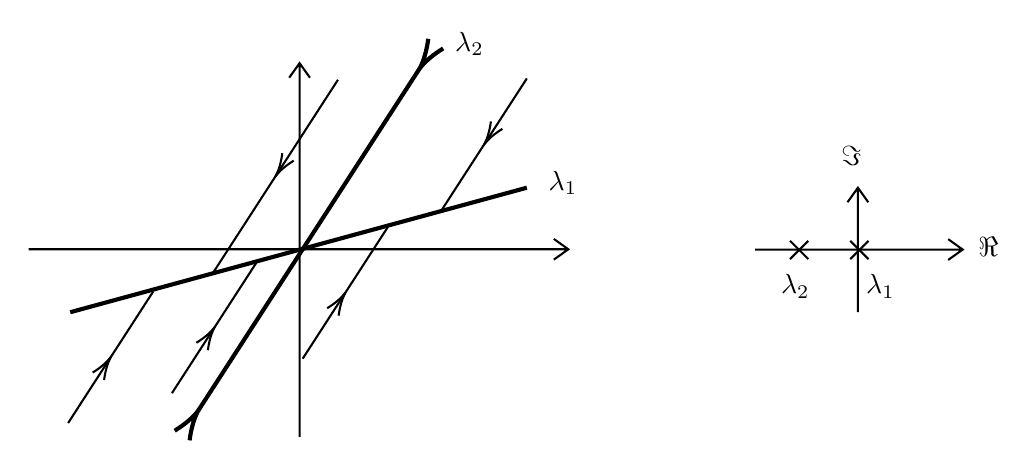
\begin{tikzpicture}[x=0.75pt,y=0.75pt,yscale=-1,xscale=1]
	      		%uncomment if require: \path (0,230); %set diagram left start at 0, and has height of 230
	      		
	      		%Shape: Axis 2D [id:dp4885530495421624] 
	      		\draw  (20,119.67) -- (280,119.67)(150.5,30) -- (150.5,210) (273,114.67) -- (280,119.67) -- (273,124.67) (145.5,37) -- (150.5,30) -- (155.5,37)  ;
	      		\draw [line width=1.5]    (208.37,32.52) -- (101.63,197.48) ;
	      		\draw [shift={(101.63,197.48)}, rotate = 122.91] [color={rgb, 255:red, 0; green, 0; blue, 0 }  ][line width=1.5]    (14.21,-4.28) .. controls (9.04,-1.82) and (4.3,-0.39) .. (0,0) .. controls (4.3,0.39) and (9.04,1.82) .. (14.21,4.28)   ;
	      		\draw [shift={(208.37,32.52)}, rotate = 302.90999999999997] [color={rgb, 255:red, 0; green, 0; blue, 0 }  ][line width=1.5]    (14.21,-4.28) .. controls (9.04,-1.82) and (4.3,-0.39) .. (0,0) .. controls (4.3,0.39) and (9.04,1.82) .. (14.21,4.28)   ;
	      		\draw [line width=1.5]    (260,90) -- (40,150) ;
	      		%Shape: Axis 2D [id:dp4297363456706407] 
	      		\draw  (370,119.8) -- (470,119.8)(419.5,90) -- (419.5,150) (463,114.8) -- (470,119.8) -- (463,124.8) (414.5,97) -- (419.5,90) -- (424.5,97)  ;
	      		\draw   (386.82,115.61) -- (395.61,124.39)(395.61,115.61) -- (386.82,124.39) ;
	      		\draw   (415.82,115.61) -- (424.61,124.39)(424.61,115.61) -- (415.82,124.39) ;
	      		\draw [line width=0.75]    (169,38) -- (109,130.73) ;
	      		\draw [shift={(139,84.36)}, rotate = 302.90999999999997] [color={rgb, 255:red, 0; green, 0; blue, 0 }  ][line width=0.75]    (10.93,-3.29) .. controls (6.95,-1.4) and (3.31,-0.3) .. (0,0) .. controls (3.31,0.3) and (6.95,1.4) .. (10.93,3.29)   ;
	      		\draw [line width=0.75]    (260,37.36) -- (219,100.73) ;
	      		\draw [shift={(239.5,69.05)}, rotate = 302.90999999999997] [color={rgb, 255:red, 0; green, 0; blue, 0 }  ][line width=0.75]    (10.93,-3.29) .. controls (6.95,-1.4) and (3.31,-0.3) .. (0,0) .. controls (3.31,0.3) and (6.95,1.4) .. (10.93,3.29)   ;
	      		\draw [line width=0.75]    (193,109) -- (152,172.36) ;
	      		\draw [shift={(172.5,140.68)}, rotate = 122.91] [color={rgb, 255:red, 0; green, 0; blue, 0 }  ][line width=0.75]    (10.93,-3.29) .. controls (6.95,-1.4) and (3.31,-0.3) .. (0,0) .. controls (3.31,0.3) and (6.95,1.4) .. (10.93,3.29)   ;
	      		\draw [line width=0.75]    (80,140) -- (39,203.36) ;
	      		\draw [shift={(59.5,171.68)}, rotate = 122.91] [color={rgb, 255:red, 0; green, 0; blue, 0 }  ][line width=0.75]    (10.93,-3.29) .. controls (6.95,-1.4) and (3.31,-0.3) .. (0,0) .. controls (3.31,0.3) and (6.95,1.4) .. (10.93,3.29)   ;
	      		\draw [line width=0.75]    (130,125.64) -- (89,189) ;
	      		\draw [shift={(109.5,157.32)}, rotate = 122.91] [color={rgb, 255:red, 0; green, 0; blue, 0 }  ][line width=0.75]    (10.93,-3.29) .. controls (6.95,-1.4) and (3.31,-0.3) .. (0,0) .. controls (3.31,0.3) and (6.95,1.4) .. (10.93,3.29)   ;
	      		
	      		\draw (269,80.4) node [anchor=north west][inner sep=0.75pt]    {$\lambda _1$};
	      		\draw (224,13.4) node [anchor=north west][inner sep=0.75pt]    {$\lambda _2$};
	      		\draw (476,112.4) node [anchor=north west][inner sep=0.75pt]    {$\Re$};
	      		\draw (410,68.4) node [anchor=north west][inner sep=0.75pt]    {$\Im$};
	      		\draw (422,130.4) node [anchor=north west][inner sep=0.75pt]    {$\lambda _1$};
	      		\draw (381,130.4) node [anchor=north west][inner sep=0.75pt]    {$\lambda _2$};
	      		
	      		
	      	\end{tikzpicture}
	      \end{figure}\FloatBarrier
	      
	\item \textbf{Autovalori negativi, coincidenti.} Qui si deve distinguere se $A$ è diagonalizzabile o meno. È simile, rispettivamente, a una di queste due matrici.\begin{equation*}
	      \tilde{A}_1 =\begin{bmatrix}
	      \lambda  & 0\\
	      0 & \lambda 
	\end{bmatrix} \ \ \ \ \tilde{A}_2 =\begin{bmatrix}
	\lambda  & 1\\
	0 & \lambda 
	\end{bmatrix}
	\end{equation*}
	\begin{itemize}
		\item Nel primo caso, l'equazione agli autovettori è $\tilde{A} x=\lambda x\implies \lambda Ix=\lambda x$, tutti i punti si trovano su degli autovettori. Si dice \textit{nodo stellato}.
		      
		      \begin{figure}[htpb]\centering
		      	\tikzset{every picture/.style={line width=0.75pt}} %set default line width to 0.75pt        
		      	
		      	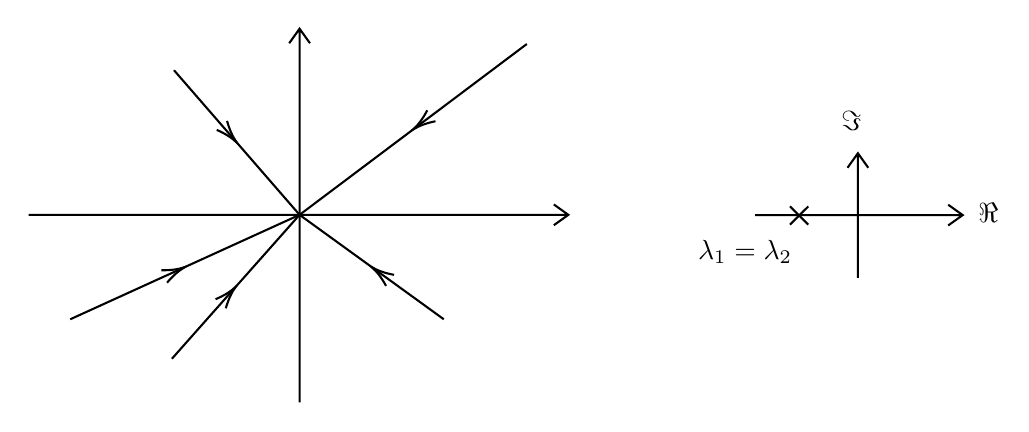
\begin{tikzpicture}[x=0.75pt,y=0.75pt,yscale=-1,xscale=1]
		      		%uncomment if require: \path (0,230); %set diagram left start at 0, and has height of 230
		      		
		      		%Shape: Axis 2D [id:dp791593271097202] 
		      		\draw  (20,119.67) -- (280,119.67)(150.5,30) -- (150.5,210) (273,114.67) -- (280,119.67) -- (273,124.67) (145.5,37) -- (150.5,30) -- (155.5,37)  ;
		      		%Shape: Axis 2D [id:dp9362413079111027] 
		      		\draw  (370,119.8) -- (470,119.8)(419.5,90) -- (419.5,150) (463,114.8) -- (470,119.8) -- (463,124.8) (414.5,97) -- (419.5,90) -- (424.5,97)  ;
		      		\draw   (386.82,115.61) -- (395.61,124.39)(395.61,115.61) -- (386.82,124.39) ;
		      		\draw [line width=0.75]    (90,50) -- (150.5,119.67) ;
		      		\draw [shift={(120.25,84.84)}, rotate = 229.03] [color={rgb, 255:red, 0; green, 0; blue, 0 }  ][line width=0.75]    (10.93,-3.29) .. controls (6.95,-1.4) and (3.31,-0.3) .. (0,0) .. controls (3.31,0.3) and (6.95,1.4) .. (10.93,3.29)   ;
		      		\draw [line width=0.75]    (260,37.36) -- (150.5,119.67) ;
		      		\draw [shift={(205.25,78.52)}, rotate = 323.07] [color={rgb, 255:red, 0; green, 0; blue, 0 }  ][line width=0.75]    (10.93,-3.29) .. controls (6.95,-1.4) and (3.31,-0.3) .. (0,0) .. controls (3.31,0.3) and (6.95,1.4) .. (10.93,3.29)   ;
		      		\draw [line width=0.75]    (150.5,119.67) -- (220,170) ;
		      		\draw [shift={(185.25,144.84)}, rotate = 35.91] [color={rgb, 255:red, 0; green, 0; blue, 0 }  ][line width=0.75]    (10.93,-3.29) .. controls (6.95,-1.4) and (3.31,-0.3) .. (0,0) .. controls (3.31,0.3) and (6.95,1.4) .. (10.93,3.29)   ;
		      		\draw [line width=0.75]    (150.5,119.67) -- (40,170) ;
		      		\draw [shift={(95.25,144.84)}, rotate = 155.51] [color={rgb, 255:red, 0; green, 0; blue, 0 }  ][line width=0.75]    (10.93,-3.29) .. controls (6.95,-1.4) and (3.31,-0.3) .. (0,0) .. controls (3.31,0.3) and (6.95,1.4) .. (10.93,3.29)   ;
		      		\draw [line width=0.75]    (150.5,119.67) -- (89,189) ;
		      		\draw [shift={(119.75,154.34)}, rotate = 131.58] [color={rgb, 255:red, 0; green, 0; blue, 0 }  ][line width=0.75]    (10.93,-3.29) .. controls (6.95,-1.4) and (3.31,-0.3) .. (0,0) .. controls (3.31,0.3) and (6.95,1.4) .. (10.93,3.29)   ;
		      		
		      		\draw (476,112.4) node [anchor=north west][inner sep=0.75pt]    {$\Re$};
		      		\draw (410,68.4) node [anchor=north west][inner sep=0.75pt]    {$\Im$};
		      		\draw (341,130.4) node [anchor=north west][inner sep=0.75pt]    {$\lambda _1 =\lambda _2$};
		      		
		      		
		      	\end{tikzpicture}
		      \end{figure}\FloatBarrier
		      
		\item Nel secondo caso, si ha un solo autovettore.
		      
		      \begin{figure}[htpb]\centering
		      	\tikzset{every picture/.style={line width=0.75pt}} %set default line width to 0.75pt        
		      	
		      	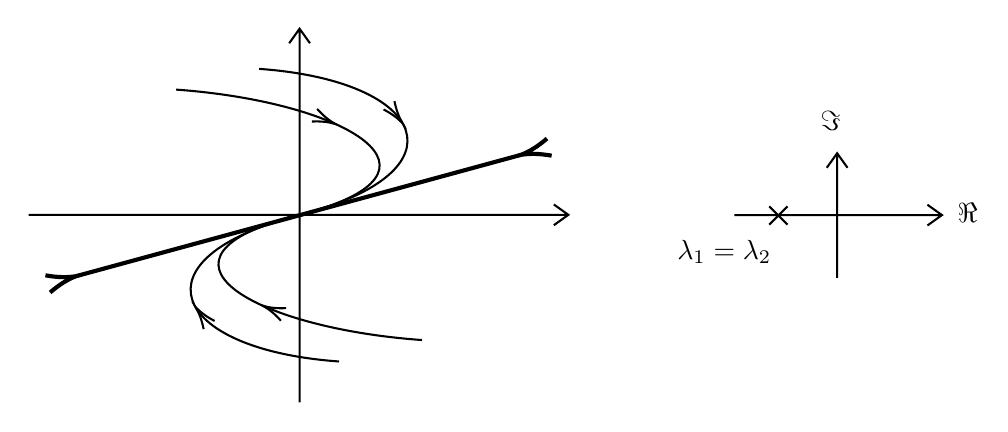
\begin{tikzpicture}[x=0.75pt,y=0.75pt,yscale=-1,xscale=1]
		      		%uncomment if require: \path (0,230); %set diagram left start at 0, and has height of 230
		      		
		      		%Shape: Axis 2D [id:dp9741804307845028] 
		      		\draw  (20,119.67) -- (280,119.67)(150.5,30) -- (150.5,210) (273,114.67) -- (280,119.67) -- (273,124.67) (145.5,37) -- (150.5,30) -- (155.5,37)  ;
		      		\draw [line width=1.5]    (257.11,90.79) -- (42.89,149.21) ;
		      		\draw [shift={(42.89,149.21)}, rotate = 164.74] [color={rgb, 255:red, 0; green, 0; blue, 0 }  ][line width=1.5]    (14.21,-4.28) .. controls (9.04,-1.82) and (4.3,-0.39) .. (0,0) .. controls (4.3,0.39) and (9.04,1.82) .. (14.21,4.28)   ;
		      		\draw [shift={(257.11,90.79)}, rotate = 344.74] [color={rgb, 255:red, 0; green, 0; blue, 0 }  ][line width=1.5]    (14.21,-4.28) .. controls (9.04,-1.82) and (4.3,-0.39) .. (0,0) .. controls (4.3,0.39) and (9.04,1.82) .. (14.21,4.28)   ;
		      		%Shape: Axis 2D [id:dp6118166731687262] 
		      		\draw  (360,119.8) -- (460,119.8)(409.5,90) -- (409.5,150) (453,114.8) -- (460,119.8) -- (453,124.8) (404.5,97) -- (409.5,90) -- (414.5,97)  ;
		      		\draw   (376.82,115.61) -- (385.61,124.39)(385.61,115.61) -- (376.82,124.39) ;
		      		%Curve Lines [id:da16205346243364738] 
		      		\draw    (169.5,190.33) .. controls (87.5,184.48) and (69.5,140.48) .. (150,120) ;
		      		\draw [shift={(100.33,164.05)}, rotate = 412.94] [color={rgb, 255:red, 0; green, 0; blue, 0 }  ][line width=0.75]    (10.93,-3.29) .. controls (6.95,-1.4) and (3.31,-0.3) .. (0,0) .. controls (3.31,0.3) and (6.95,1.4) .. (10.93,3.29)   ;
		      		%Curve Lines [id:da3209569303580111] 
		      		\draw    (209.5,180) .. controls (127.5,174.16) and (69.5,140.16) .. (150,119.67) ;
		      		\draw [shift={(132.7,163.43)}, rotate = 382.75] [color={rgb, 255:red, 0; green, 0; blue, 0 }  ][line width=0.75]    (10.93,-3.29) .. controls (6.95,-1.4) and (3.31,-0.3) .. (0,0) .. controls (3.31,0.3) and (6.95,1.4) .. (10.93,3.29)   ;
		      		%Curve Lines [id:da3583891764638174] 
		      		\draw    (131,49.34) .. controls (213,55.19) and (231,99.19) .. (150.5,119.67) ;
		      		\draw [shift={(200.17,75.63)}, rotate = 232.94] [color={rgb, 255:red, 0; green, 0; blue, 0 }  ][line width=0.75]    (10.93,-3.29) .. controls (6.95,-1.4) and (3.31,-0.3) .. (0,0) .. controls (3.31,0.3) and (6.95,1.4) .. (10.93,3.29)   ;
		      		%Curve Lines [id:da8351151210758669] 
		      		\draw    (91,59.34) .. controls (173,65.19) and (231,99.19) .. (150.5,119.67) ;
		      		\draw [shift={(167.8,75.92)}, rotate = 202.75] [color={rgb, 255:red, 0; green, 0; blue, 0 }  ][line width=0.75]    (10.93,-3.29) .. controls (6.95,-1.4) and (3.31,-0.3) .. (0,0) .. controls (3.31,0.3) and (6.95,1.4) .. (10.93,3.29)   ;
		      		
		      		\draw (466,112.4) node [anchor=north west][inner sep=0.75pt]    {$\Re$};
		      		\draw (400,68.4) node [anchor=north west][inner sep=0.75pt]    {$\Im$};
		      		\draw (331,130.4) node [anchor=north west][inner sep=0.75pt]    {$\lambda _1 =\lambda _2$};
		      		
		      		
		      	\end{tikzpicture}
		      \end{figure}\FloatBarrier
		      
	\end{itemize}
	\item \textbf{Autovettori complessi.} Si ha una dinamica oscillatoria, la configurazione dipende dalla parte reale degli autovalori. Se è negativa si ha un \textit{fuoco stabile}, se è positiva si ha un \textit{fuoco instabile}, se è nulla si ha un \textit{centro}.
	      
	      \begin{figure}[htpb]\centering
	      	\tikzset{every picture/.style={line width=0.75pt}} %set default line width to 0.75pt        
	      	
	      	\begin{tikzpicture}[x=0.75pt,y=0.75pt,yscale=-1,xscale=1]
	      		%uncomment if require: \path (0,230); %set diagram left start at 0, and has height of 230
	      		
	      		%Shape: Axis 2D [id:dp49475614171774707] 
	      		\draw  (20,119.67) -- (280,119.67)(150.5,30) -- (150.5,210) (273,114.67) -- (280,119.67) -- (273,124.67) (145.5,37) -- (150.5,30) -- (155.5,37)  ;
	      		%Shape: Axis 2D [id:dp020318598732544713] 
	      		\draw  (380,119.8) -- (480,119.8)(429.5,90) -- (429.5,150) (473,114.8) -- (480,119.8) -- (473,124.8) (424.5,97) -- (429.5,90) -- (434.5,97)  ;
	      		%Curve Lines [id:da755033161296657] 
	      		\draw    (130,60) .. controls (40.5,108.48) and (99.5,180.52) .. (160,150) .. controls (220.5,119.48) and (167.5,70.48) .. (140,90) .. controls (112.5,109.52) and (130.5,134.67) .. (150.5,119.67) ;
	      		\draw [shift={(85.99,128.27)}, rotate = 256.93] [color={rgb, 255:red, 0; green, 0; blue, 0 }  ][line width=0.75]    (10.93,-3.29) .. controls (6.95,-1.4) and (3.31,-0.3) .. (0,0) .. controls (3.31,0.3) and (6.95,1.4) .. (10.93,3.29)   ;
	      		\draw [shift={(185.96,106.85)}, rotate = 434.6] [color={rgb, 255:red, 0; green, 0; blue, 0 }  ][line width=0.75]    (10.93,-3.29) .. controls (6.95,-1.4) and (3.31,-0.3) .. (0,0) .. controls (3.31,0.3) and (6.95,1.4) .. (10.93,3.29)   ;
	      		\draw [shift={(126.36,114.9)}, rotate = 267.98] [color={rgb, 255:red, 0; green, 0; blue, 0 }  ][line width=0.75]    (10.93,-3.29) .. controls (6.95,-1.4) and (3.31,-0.3) .. (0,0) .. controls (3.31,0.3) and (6.95,1.4) .. (10.93,3.29)   ;
	      		\draw  [dash pattern={on 0.84pt off 2.51pt}]  (400,100) -- (400,140) ;
	      		\draw [shift={(400,140)}, rotate = 135] [color={rgb, 255:red, 0; green, 0; blue, 0 }  ][line width=0.75]    (-5.59,0) -- (5.59,0)(0,5.59) -- (0,-5.59)   ;
	      		\draw [shift={(400,100)}, rotate = 135] [color={rgb, 255:red, 0; green, 0; blue, 0 }  ][line width=0.75]    (-5.59,0) -- (5.59,0)(0,5.59) -- (0,-5.59)   ;
	      		
	      		\draw (486,112.4) node [anchor=north west][inner sep=0.75pt]    {$\Re$};
	      		\draw (420,68.4) node [anchor=north west][inner sep=0.75pt]    {$\Im$};
	      		
	      		
	      	\end{tikzpicture}
	      \end{figure}\FloatBarrier
	      
	      
	      \begin{figure}[htpb]\centering
	      	\tikzset{every picture/.style={line width=0.75pt}} %set default line width to 0.75pt        
	      	
	      	\begin{tikzpicture}[x=0.75pt,y=0.75pt,yscale=-1,xscale=1]
	      		%uncomment if require: \path (0,230); %set diagram left start at 0, and has height of 230
	      		
	      		%Shape: Axis 2D [id:dp7353345560066575] 
	      		\draw  (20,119.67) -- (280,119.67)(150.5,30) -- (150.5,210) (273,114.67) -- (280,119.67) -- (273,124.67) (145.5,37) -- (150.5,30) -- (155.5,37)  ;
	      		%Shape: Axis 2D [id:dp7712792485486917] 
	      		\draw  (380,119.8) -- (480,119.8)(429.5,90) -- (429.5,150) (473,114.8) -- (480,119.8) -- (473,124.8) (424.5,97) -- (429.5,90) -- (434.5,97)  ;
	      		%Curve Lines [id:da4430242814821286] 
	      		\draw    (130,60) .. controls (40.5,108.48) and (99.5,180.52) .. (160,150) .. controls (220.5,119.48) and (167.5,70.48) .. (140,90) .. controls (112.5,109.52) and (130.5,134.67) .. (150.5,119.67) ;
	      		\draw [shift={(85.99,128.27)}, rotate = 76.93] [color={rgb, 255:red, 0; green, 0; blue, 0 }  ][line width=0.75]    (10.93,-3.29) .. controls (6.95,-1.4) and (3.31,-0.3) .. (0,0) .. controls (3.31,0.3) and (6.95,1.4) .. (10.93,3.29)   ;
	      		\draw [shift={(185.96,106.85)}, rotate = 254.6] [color={rgb, 255:red, 0; green, 0; blue, 0 }  ][line width=0.75]    (10.93,-3.29) .. controls (6.95,-1.4) and (3.31,-0.3) .. (0,0) .. controls (3.31,0.3) and (6.95,1.4) .. (10.93,3.29)   ;
	      		\draw [shift={(126.36,114.9)}, rotate = 87.98] [color={rgb, 255:red, 0; green, 0; blue, 0 }  ][line width=0.75]    (10.93,-3.29) .. controls (6.95,-1.4) and (3.31,-0.3) .. (0,0) .. controls (3.31,0.3) and (6.95,1.4) .. (10.93,3.29)   ;
	      		\draw  [dash pattern={on 0.84pt off 2.51pt}]  (450,100) -- (450,140) ;
	      		\draw [shift={(450,140)}, rotate = 135] [color={rgb, 255:red, 0; green, 0; blue, 0 }  ][line width=0.75]    (-5.59,0) -- (5.59,0)(0,5.59) -- (0,-5.59)   ;
	      		\draw [shift={(450,100)}, rotate = 135] [color={rgb, 255:red, 0; green, 0; blue, 0 }  ][line width=0.75]    (-5.59,0) -- (5.59,0)(0,5.59) -- (0,-5.59)   ;
	      		
	      		\draw (486,112.4) node [anchor=north west][inner sep=0.75pt]    {$\Re$};
	      		\draw (420,68.4) node [anchor=north west][inner sep=0.75pt]    {$\Im$};
	      		
	      		
	      	\end{tikzpicture}
	      \end{figure}\FloatBarrier
	      
	      
	      \begin{figure}[htpb]\centering
	      	\tikzset{every picture/.style={line width=0.75pt}} %set default line width to 0.75pt        
	      	
	      	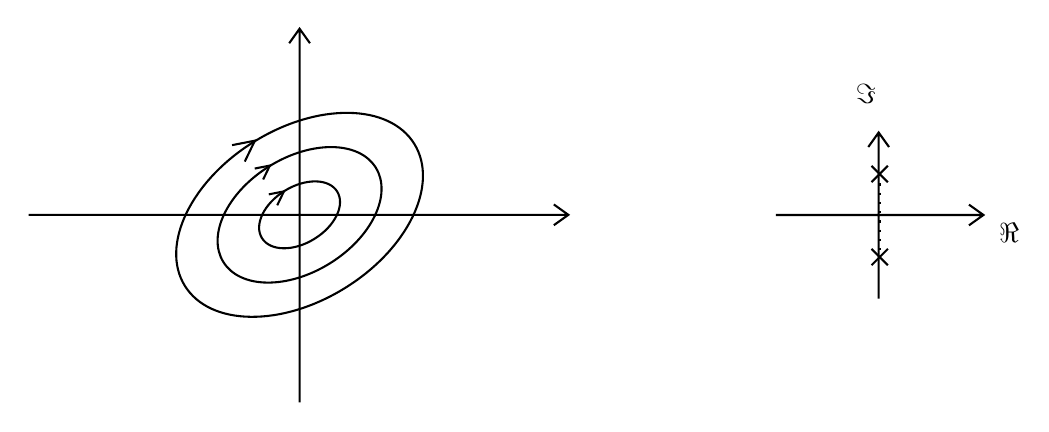
\begin{tikzpicture}[x=0.75pt,y=0.75pt,yscale=-1,xscale=1]
	      		%uncomment if require: \path (0,230); %set diagram left start at 0, and has height of 230
	      		
	      		%Shape: Axis 2D [id:dp5066227070439475] 
	      		\draw  (20,119.67) -- (280,119.67)(150.5,30) -- (150.5,210) (273,114.67) -- (280,119.67) -- (273,124.67) (145.5,37) -- (150.5,30) -- (155.5,37)  ;
	      		%Shape: Axis 2D [id:dp6378475471355132] 
	      		\draw  (380,119.74) -- (480,119.74)(429.5,80) -- (429.5,160) (473,114.74) -- (480,119.74) -- (473,124.74) (424.5,87) -- (429.5,80) -- (434.5,87)  ;
	      		\draw  [dash pattern={on 0.84pt off 2.51pt}]  (430,100) -- (430,140) ;
	      		\draw [shift={(430,140)}, rotate = 135] [color={rgb, 255:red, 0; green, 0; blue, 0 }  ][line width=0.75]    (-5.59,0) -- (5.59,0)(0,5.59) -- (0,-5.59)   ;
	      		\draw [shift={(430,100)}, rotate = 135] [color={rgb, 255:red, 0; green, 0; blue, 0 }  ][line width=0.75]    (-5.59,0) -- (5.59,0)(0,5.59) -- (0,-5.59)   ;
	      		%Shape: Ellipse [id:dp6467250166159959] 
	      		\draw   (95.22,153.86) .. controls (83.16,134.36) and (98.14,103.25) .. (128.67,84.37) .. controls (159.21,65.49) and (193.73,65.99) .. (205.78,85.49) .. controls (217.84,104.98) and (202.86,136.09) .. (172.33,154.97) .. controls (141.79,173.85) and (107.27,173.35) .. (95.22,153.86) -- cycle ;
	      		\draw   (117.99,86.1) -- (128.96,83.94) -- (124.1,94.01) ;
	      		%Shape: Ellipse [id:dp012915694760300855] 
	      		\draw   (113.77,142.38) .. controls (105.76,129.43) and (115.71,108.76) .. (136,96.22) .. controls (156.29,83.68) and (179.22,84.01) .. (187.23,96.96) .. controls (195.24,109.91) and (185.29,130.58) .. (165,143.12) .. controls (144.71,155.67) and (121.78,155.34) .. (113.77,142.38) -- cycle ;
	      		\draw   (128.9,97.37) -- (136.19,95.93) -- (132.96,102.63) ;
	      		%Shape: Ellipse [id:dp21515527321369143] 
	      		\draw   (132.37,130.88) .. controls (128.41,124.49) and (133.33,114.29) .. (143.34,108.09) .. controls (153.36,101.9) and (164.68,102.07) .. (168.63,108.46) .. controls (172.59,114.85) and (167.67,125.06) .. (157.66,131.25) .. controls (147.64,137.44) and (136.32,137.28) .. (132.37,130.88) -- cycle ;
	      		\draw   (135.68,109.81) -- (142.97,108.37) -- (139.74,115.06) ;
	      		
	      		\draw (486,122.4) node [anchor=north west][inner sep=0.75pt]    {$\Re$};
	      		\draw (417,55.4) node [anchor=north west][inner sep=0.75pt]    {$\Im$};
	      		
	      		
	      	\end{tikzpicture}
	      \end{figure}\FloatBarrier
	      
\end{itemize}

In dimensione $3$ si può ragionare analogamente.

\chapter{Sistemi non lineari}

Ricordiamo che in generale i sistemi si scrivono come
\begin{gather*}
	\dot{x}(t) =f(x(t) ,u(t))\\
	x(t+1) =f(x(t) ,u(t))\\
    y = g(x(t),u(t))
\end{gather*}
%Rinnoviamo l'ipotesi di ingresso costante $u(t) =\overline{u} \ \forall t\geq 0$. Dato che lo possiamo considerare come un parametro, studieremo
%\begin{gather*}
%	\dot{x}(t) =f(x(t))\\
%	x(t+1) =f(x(t))
%\end{gather*}

\section{Equilibrio: esistenza e unicità}

Gli equilibri, analogamente ai sistemi lineari, li troviamo imponendo
\begin{gather*}
	f(x(t)) =0\\
	f(x(t)) =x
\end{gather*}

\section{Stabilità dell'equilibrio}

La trattazione di equilibrio è dovuta a Lyapunov. Un equilibrio $\overline x$ è
\begin{itemize}
	\item \textbf{stabile} se $\forall \varepsilon  >0\ \exists \delta _{\varepsilon }  >0$ tale che\begin{equation*}
	      \Vert x(0) -\overline{x}\Vert < \delta _{\varepsilon } \implies \Vert x(t) -\overline{x}\Vert < \varepsilon \ \ \forall x(0) :\Vert x(0) -\overline{x}\Vert < \delta _{\varepsilon } ,\forall t\geq 0
	\end{equation*}
	
	cioè tale per cui per stati iniziali vicini all'equilibrio, non mi allontano
	\item \textbf{asintoticamente stabile} se
	      \begin{itemize}
	      	\item è stabile
	      	\item $\lim\limits _{t\to \infty } x(t) =\overline{x} \ \forall x(0) :\Vert x(0) -\overline{x}\Vert < \delta _{\varepsilon }$
	      \end{itemize}
	      
	      Sono un sottoinsieme di quelli stabili. Col passare del tempo non solo non mi devo allontanare, ma mi devo riavvicinare all'equilibrio.
	\item \textbf{instabile} se non è stabile
\end{itemize}

Se un equilibrio è asint. stabile si definisce il suo \textbf{bacino di attrazione}
\begin{equation*}
	B(\overline{x}) =\left\{x(0) :x(t)\to \overline{x}\right\}
\end{equation*}
Si può poi dire che $\overline{x}$ asint. stabile è \textbf{globalmente stabile} se $B(\overline{x}) =\mathbb{R}^n$, ma possiamo dare una definizione più morbida: $\overline{x}$ asint. stabile è \textbf{quasi globalmente stabile} se $B(\overline{x}) =\mathbb{R}^n$ a meno di un insieme di misura nulla.

Nei sistemi non lineari la classificazione è diversa dai sistemi lineari:

\begin{figure}[htpb]\centering
	\tikzset{every picture/.style={line width=0.75pt}} %set default line width to 0.75pt        
	
	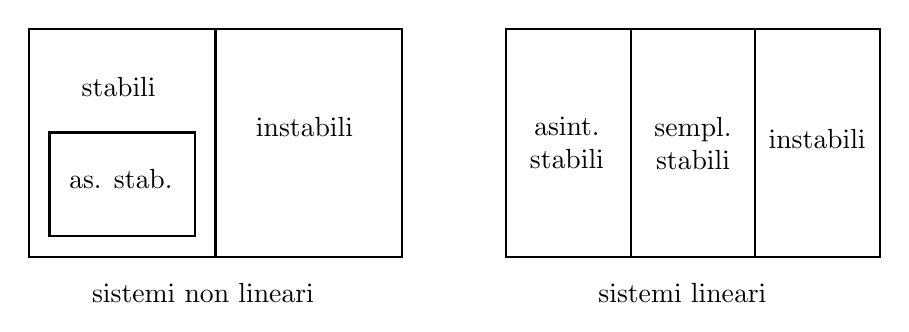
\begin{tikzpicture}[x=0.75pt,y=0.75pt,yscale=-1,xscale=1]
		%uncomment if require: \path (0,168); %set diagram left start at 0, and has height of 168
		
		%Shape: Rectangle [id:dp045767532386027154] 
		\draw   (80,20) -- (260,20) -- (260,130) -- (80,130) -- cycle ;
		%Shape: Rectangle [id:dp043719183492401115] 
		\draw   (90,70) -- (160,70) -- (160,120) -- (90,120) -- cycle ;
		\draw    (170,20) -- (170,130) ;
		%Shape: Rectangle [id:dp24897861156163592] 
		\draw   (310,20) -- (370,20) -- (370,130) -- (310,130) -- cycle ;
		%Shape: Rectangle [id:dp024746479119179376] 
		\draw   (430,20) -- (490,20) -- (490,130) -- (430,130) -- cycle ;
		%Shape: Rectangle [id:dp41899824839722366] 
		\draw   (370,20) -- (430,20) -- (430,130) -- (370,130) -- cycle ;
		
		\draw (104,42) node [anchor=north west][inner sep=0.75pt]   [align=left] {stabili};
		\draw (98,86) node [anchor=north west][inner sep=0.75pt]   [align=left] {as. stab.};
		\draw (188,61) node [anchor=north west][inner sep=0.75pt]   [align=left] {instabili};
		\draw (320,61) node [anchor=north west][inner sep=0.75pt]   [align=center] {asint.\\stabili};
		\draw (380,61) node [anchor=north west][inner sep=0.75pt]   [align=center] {sempl.\\stabili};
		\draw (435,67) node [anchor=north west][inner sep=0.75pt]   [align=center] {instabili};
		\draw (109,141) node [anchor=north west][inner sep=0.75pt]   [align=left] {sistemi non lineari};
		\draw (353,141) node [anchor=north west][inner sep=0.75pt]   [align=left] {sistemi lineari};
		
		
	\end{tikzpicture}
\end{figure}\FloatBarrier

\textit{Nei sistemi lineari la stabilità è attributo del sistema, nei sistemi non lineari la stabilità è attributo dell'equilibrio.}

Si presenta una casistica, i cui primi $3$ casi erano presenti anche per i sistemi lineari
\begin{itemize}
	\item $\nexists \overline{x}$, non esistono equilibri (pallina su superficie obliqua)
	\item $\exists !\overline{x}$, equilibrio unico (pallina in una conca)
	\item $\exists \infty \overline{x}$, infiniti (non numerabili) equilibri (pallina in piano)
	\item $\exists $ un numero finito maggiore di $1$ di equilibri $\overline{x}$ (più conche)
	\item $\exists \infty \overline{x}$, infiniti (numerabili) di equilibri (infinite conche)
\end{itemize}

\textit{Esempio: crescita logistica. }Parto dal modello di Malthus e arrivo alla crescita logistica. Sia $x(t)$ la dimensione della popolazione.
\begin{equation*}
	\dot{x}(t) =rx(t) ,\ r >0\ \ \implies \ \ x(t) =e^{rt} x(0)
\end{equation*}
La popolazione crescerebbe all'infinito, ma le risorse dopo un po' scarseggiano, quindi non è lecito supporre $r$ costante, ma dipende da $x$ e descresce con essa.
\begin{equation*}
	r=r_0\left(1-\frac{x}{k}\right)
\end{equation*}
Quindi la relazione diventa
\begin{equation*}
	\dot{x}(t) =r_0\left(1-\frac{x}{k}\right) x=f(x)
\end{equation*}
non è lineare. Siamo nel caso di $2$ equilibri: $\overline{x} =0,\overline{x} =k$. Matematicamente se siamo tra $0$ e $k$, $f(x)$ è positiva, quindi $\dot{x}(t)$. Invece se siamo oltre $k$ uno dei due fattori diventa negativo e quindi $\dot{x}(t)$. Ipotizzando di considerare anche $x$ negativi, si deduce anche che $0$ è un equilibrio instabile. $k$ è un equilibrio stabile, viene detto capacità portante. Il bacino di attrazione di $\overline{x} =k$ è $B(\overline{x}) =\mathbb{R}_{+}$.

\section{Isocline}

Studiare le isocline significa studiare
\begin{equation*}
	f_i(x_1 ,x_2) =k
\end{equation*}
Nello specifico, se studiamo il caso $k=0$, stiamo sostanzialmente cercando i punti a tangente nulla rispetto a una specifica variabile.

\section{Metodo di linearizzazione}

Vediamo il caso a tempo continuo. Sia $\dot{x}(t) =f(x(t),u(t)) ,\dot{x} \in \mathbb{R}^n$ e sia $\overline{x} :f(\overline{x},\overline{u}) =0$ uno stato di equilibrio. Consideriamo $z(t) =x(t) -\overline{x}$ e $v(t)=u(t)-\overline{u}$. Si ha
\begin{equation*}
	\dot{z} =\dot{x} =f(x,\overline{u})=f(z+\overline{x},v+\overline{u})
\end{equation*}
Facciamo lo sviluppo di Taylor nell'intorno di $(\overline{x},\overline{u})$
\begin{equation*}
	\dot{z} =\underbrace{f(\overline{x},\overline{u})}_{=0} +\left. \frac{\partial f}{\partial x}\right| _{x=\overline{x},u=\overline{u}} z+\left. \frac{\partial f}{\partial u}\right| _{x=\overline{x},u=\overline{u}} v+\cdots =:A(\overline{x},\overline{u}) z+b(\overline{x},\overline{u})v+\cdots 
\end{equation*}
dove
\begin{equation*}
	\frac{\partial f}{\partial x} =A(\overline{x},\overline{u})=\left.\begin{bmatrix}
	\frac{\partial f_1}{\partial x_1} & \frac{\partial f_1}{\partial x_2} & \cdots  & \frac{\partial f_1}{\partial x_n}\\
	\frac{\partial f_2}{\partial x_1} & \frac{\partial f_2}{\partial x_2} & \dotsc  & \frac{\partial f_2}{\partial x_n}\\
	\vdots  & \vdots  & \ddots  & \vdots \\
	\frac{\partial f_n}{\partial x_1} & \frac{\partial f_n}{\partial x_2} & \cdots  & \frac{\partial f_n}{\partial x_n}
	\end{bmatrix}\right |_{\overline{x},\overline{u}} \in \mathbb{R}^{n\times n},\quad \frac{\partial f}{\partial u}=b(\overline{x},\overline{u})=\left.\begin{bmatrix}
	    \partial f_1\over \partial u\\
        \partial f_2\over \partial u\\
        \vdots\\
        \partial f_n \over \partial u
	\end{bmatrix}\right|_{\overline{x},\overline{u}}
\end{equation*}
$A$ è la \textbf{matrice jacobiana} privata dell'ultima colonna, mentre $b$ è l'ultima colonna della matrice jacobiana. Butto via i termini superiori al primo, e definisco il \textbf{sistema linearizzato nell'intorno di }$(\overline{x},\overline{u})$
\begin{equation*}
	\boxed{\dot{z} =A(\overline{x},\overline{u}) z(t)+b(\overline x,\overline u)v(t)}
\end{equation*}
Consideriamo ora $\dot{x} =f(x)$ con $\overline{x}$ equilibrio e il suo sistema linearizzato $\dot{z} =A(\overline{x}) z$. Dobbiamo introdurre il concetto di varietà, ne esistono tre tipi
\begin{itemize}
	\item stabile
	\item instabile
	\item centro
\end{itemize}

È un insieme definito, in $\mathbb{R}^n$, localmente nell'intorno di un punto, tale da essere localmente in corrispondenza biunivoca con uno spazio di $\mathbb{R}^m ,m\leq n$. Per esempio una curva in un piano.

Gli autovalori del sistema linearizzato sono
\begin{equation*}
	\sigma (A(\overline{x})) =\{\lambda _1 ,\dotsc ,\lambda _n\}
\end{equation*}
e li partizioniamo in base al segno della loro parte reale
\begin{itemize}
	\item ce ne sono $n^{-}$ con $\Re(\lambda) < 0$
	\item ce ne sono $n^{+}$ con $\Re(\lambda)  >0$
	\item ce ne sono $n^0$ con $\Re(\lambda) =0$
\end{itemize}

ovviamente $n^{-} +n^{+} +n^0 =n$. Si possono dimostrare i seguenti risultati
\begin{enumerate}
	\item Esistono nell'intorno di $\overline{x}$ le tre varietà
	      \begin{enumerate}
	      	\item $W^s$ varietà stabile, $\dim W^s =n^{-}$
	      	\item $W^u$ varietà instabile, $\dim W^u =n^{+}$
	      	\item $W^0$ varietà centro, $\dim W^0 =n^0$
	      \end{enumerate}
	\item $W^s ,W^u ,W^0$ includono $\overline{x}$ e sono tangenti in $\overline{x}$ alle corrispondenti varietà del sistema linearizzato
	\item $W^s ,W^u ,W^0$ sono invarianti rispetto a $\dot{x} =f(x)$
	\item Su $W^s ,W^u$ la dinamica è equivalente a quella di $\dot{z} =A(\overline{x}) z$
	\item Su $W^0$ la dinamica è governata dai termini di ordine superiore dello sviluppo di Taylor
\end{enumerate}

Vale inoltre il seguente importante risultato (non sono coimplicazioni).

\begin{thm}
	\textbf{Teorema di linearizzazione}
    \begin{itemize}
    	\item $A(\overline{x},\overline{u})$ asint. stabile $\implies $ $\overline{x}$ asint. stabile
    	\item $A(\overline{x},\overline{u})$ fortemente instabile $\implies $ $\overline{x}$ instabile
    \end{itemize}
\end{thm}

Se ci sono autovalori nulli e nessuno strettamente positivo in $A(\overline{x})$ non possiamo dire nulla su $\overline{x}$ proprio per il problema che la dinamica sulle varietà centro è governata da termini di ordine superiore al primo.

Se non ci sono autovalori nulli, ovvero non ci sono varietà centro, l'equilibro si dice anche \textit{iperbolico}.

\chapter{Raggiungibilità}

\begin{figure}[htpb]\centering
	\tikzset{every picture/.style={line width=0.75pt}} %set default line width to 0.75pt        
	
	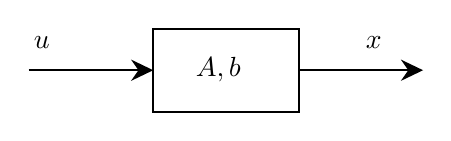
\begin{tikzpicture}[x=0.75pt,y=0.75pt,yscale=-1,xscale=1]
		%uncomment if require: \path (0,59); %set diagram left start at 0, and has height of 59
		
		%Shape: Rectangle [id:dp21780520893794053] 
		\draw   (150,10) -- (220,10) -- (220,50) -- (150,50) -- cycle ;
		\draw    (90,30) -- (147,30) ;
		\draw [shift={(150,30)}, rotate = 180] [fill={rgb, 255:red, 0; green, 0; blue, 0 }  ][line width=0.08]  [draw opacity=0] (10.72,-5.15) -- (0,0) -- (10.72,5.15) -- (7.12,0) -- cycle    ;
		\draw    (220,30) -- (277,30) ;
		\draw [shift={(280,30)}, rotate = 180] [fill={rgb, 255:red, 0; green, 0; blue, 0 }  ][line width=0.08]  [draw opacity=0] (10.72,-5.15) -- (0,0) -- (10.72,5.15) -- (7.12,0) -- cycle    ;
		
		\draw (169,22.4) node [anchor=north west][inner sep=0.75pt]    {$A,b$};
		\draw (91,12.4) node [anchor=north west][inner sep=0.75pt]    {$u$};
		\draw (251,12.4) node [anchor=north west][inner sep=0.75pt]    {$x$};
		
		
	\end{tikzpicture}
\end{figure}\FloatBarrier

Consideriamo sistemi del tipo
\begin{gather*}
	\dot{x} =Ax+bu\\
	x(t+1) =Ax(t) +bu(t)
\end{gather*}
Non ci serve mettere in evidenza l'uscita. Ci interroghiamo su come l'ingresso influenza lo stato. Ricordiamo che se conosciamo $x(0)$ e l'ingresso $u_{[ 0,t)}$ possiamo determinare lo stato e scomporlo in due parti
\begin{equation*}
	x(t) =\phi (t) x(0) +\psi (t)\left( u_{[ 0,t)}\right)
\end{equation*}
ricordiamo che $\psi $ è un operatore, non una matrice. Se $x(0) =0\implies x(t) =\psi (t)\left( u_{[ 0,t)}\right)$
\begin{defn}
	$\tilde{x}$ è uno \textbf{stato raggiungibile} all'istante $t$ se esiste $u_{[ 0,t)}$ tale che $x(t) =\tilde{x}$, con $x(0) =0$.
\end{defn}
Chiamiamo \textbf{insieme di raggiungibilità}
\begin{equation*}
	X_R(t) =\left\{\text{insieme degli} \ \tilde{x} \ \text{raggiungibili in} \ t\right\} =\Im(\psi (t)) \subseteq \mathbb{R}^n
\end{equation*}
$X_R(t)$ è un sottospazio di $\mathbb{R}^n$, quindi gode ad esempio della proprietà
\begin{equation*}
	v_1 ,v_2 \in S\implies \alpha v_1 +\beta v_2 \in S\ \ \ \ \alpha ,\beta \in \mathbb{R}
\end{equation*}
quindi sono rette, piani, iperpiani, ecc.

Un'altra proprietà è che: se $t_2  >t_1 \implies X_R(t_2) \supset X_R(t_1)$, l'insieme di raggiungibilità tende a diventare più grande, includendo sempre i precedenti. In particolare, si espande con \textit{discontinuità}.
\begin{defn}
	$(A,b)$ è completamente raggiungibile se $X_R =\mathbb{R}^n$, ovvero $\dim X_R =n$.
\end{defn}
Introduciamo la \textbf{matrice di raggiungibilità} $R$:
\begin{equation*}
	\boxed{
		R=\begin{bmatrix}
		b & Ab & A^2 b & \dotsc  & A^{n-1} b
		\end{bmatrix} \in \mathbb{R}^{n\times n}
	}
\end{equation*}
Si dimostra che
\begin{equation*}
	X_R =\Im(R) =\Span(R)
\end{equation*}
da cui si deduce anche
\begin{equation*}
	\dim(X_R) =\rank(R)
\end{equation*}
e che
\begin{equation*}
	(A,b) \ \text{compl. ragg.} \ \ \iff \ \ \rank(R) =n\ \ \iff \ \ \det R\neq 0
\end{equation*}
\textit{Dimostrazione a tempo discreto (perché più facile).}

Se parto in $x(0) =0$, cosa posso raggiungere all'istante $t=1$? Siccome $u(0)$ è arbitrario, posso raggiungere l'immagine di $b$
\begin{equation*}
	\begin{aligned}
		x(0) & =0 & \\
		x(1) & =\cancel{Ax(0)} +bu(0) & X_R(1) =\Im(b)\\
		x(2) & =Abu(0) +bu(1) & \\
		& =\begin{bmatrix}
		b & Ab
		\end{bmatrix}\begin{bmatrix}
		u(1)\\
		u(0)
		\end{bmatrix} & X_R(2) =\Im\left(\begin{bmatrix}
		b & Ab
		\end{bmatrix}\right)\\
		\vdots  &  & \\
		x(t) &  \begin{array}{l}
		=A^{t-1} bu(0) +A^{t-2} bu(1) +\\
		\ \ \ \ \cdots +Abu(t-2) +bu(t-1)
		\end{array} & \\
		& =\begin{bmatrix}
		b & Ab & \dotsc & A^{t-2} b & A^{t-1} b 
		\end{bmatrix}\begin{bmatrix}
		u(t-1)\\
		u(t-2)\\
		\vdots \\
		u(1)\\
		u(0)
		\end{bmatrix} & X_R(t) =\Im\left(\begin{bmatrix}
		b & \dotsc  & A^{t-1} b
		\end{bmatrix}\right)
	\end{aligned}
\end{equation*}
Qui si vede bene che il sottospazio tende ad espandersi, se il nuovo vettore è linearmente indipendente dagli altri. Perché ci fermiamo in $n-1$? Perché tutti quelli successivi saranno sicuramente combinazioni lineari dei precedenti. Questo vale per il teorema di Cayley-Hamilton
\begin{gather*}
	\Delta _A(\lambda) =\lambda ^n +\alpha _1 \lambda ^{n-1} +\cdots +\alpha _n\\
	\implies \Delta _A(A) =A^n +\alpha _1 A^{n-1} +\cdots +\alpha _n I=0
\end{gather*}
Possiamo moltiplicare tutto per $b$
\begin{equation*}
	A^n b+\alpha _1 A^{n-1} b+\cdots +\alpha _n b=0\ \ \implies \ \ A^n b=-\alpha _1 A^{n-1} b-\cdots -\alpha _n b
\end{equation*}
È inutile andare avanti, all'$n$-esimo iniziano a essere combinazioni dei precedenti. Tutti gli stati raggiungibili sono raggiungibili in al più $n$ passi, dopo quelli non apriamo più nuove direzioni.

\section{Legge di controllo}

\begin{figure}[htpb]\centering
	\tikzset{every picture/.style={line width=0.75pt}} %set default line width to 0.75pt        
	
	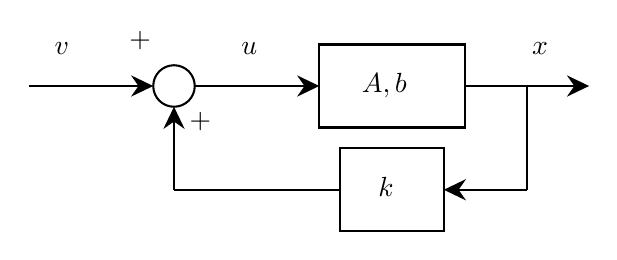
\begin{tikzpicture}[x=0.75pt,y=0.75pt,yscale=-1,xscale=1]
		%uncomment if require: \path (0,124); %set diagram left start at 0, and has height of 124
		
		%Shape: Rectangle [id:dp4437022367927297] 
		\draw   (200,20) -- (270,20) -- (270,60) -- (200,60) -- cycle ;
		\draw    (140,40) -- (197,40) ;
		\draw [shift={(200,40)}, rotate = 180] [fill={rgb, 255:red, 0; green, 0; blue, 0 }  ][line width=0.08]  [draw opacity=0] (10.72,-5.15) -- (0,0) -- (10.72,5.15) -- (7.12,0) -- cycle    ;
		\draw    (270,40) -- (327,40) ;
		\draw [shift={(330,40)}, rotate = 180] [fill={rgb, 255:red, 0; green, 0; blue, 0 }  ][line width=0.08]  [draw opacity=0] (10.72,-5.15) -- (0,0) -- (10.72,5.15) -- (7.12,0) -- cycle    ;
		%Shape: Circle [id:dp2362841862575824] 
		\draw   (120,40) .. controls (120,34.48) and (124.48,30) .. (130,30) .. controls (135.52,30) and (140,34.48) .. (140,40) .. controls (140,45.52) and (135.52,50) .. (130,50) .. controls (124.48,50) and (120,45.52) .. (120,40) -- cycle ;
		\draw    (60,40) -- (117,40) ;
		\draw [shift={(120,40)}, rotate = 180] [fill={rgb, 255:red, 0; green, 0; blue, 0 }  ][line width=0.08]  [draw opacity=0] (10.72,-5.15) -- (0,0) -- (10.72,5.15) -- (7.12,0) -- cycle    ;
		%Shape: Rectangle [id:dp7472145312569753] 
		\draw   (210,70) -- (260,70) -- (260,110) -- (210,110) -- cycle ;
		\draw    (300,40) -- (300,90) ;
		\draw    (300,90) -- (263,90) ;
		\draw [shift={(260,90)}, rotate = 360] [fill={rgb, 255:red, 0; green, 0; blue, 0 }  ][line width=0.08]  [draw opacity=0] (10.72,-5.15) -- (0,0) -- (10.72,5.15) -- (7.12,0) -- cycle    ;
		\draw    (210,90) -- (130,90) ;
		\draw    (130,90) -- (130,53) ;
		\draw [shift={(130,50)}, rotate = 450] [fill={rgb, 255:red, 0; green, 0; blue, 0 }  ][line width=0.08]  [draw opacity=0] (10.72,-5.15) -- (0,0) -- (10.72,5.15) -- (7.12,0) -- cycle    ;
		
		\draw (219,32.4) node [anchor=north west][inner sep=0.75pt]    {$A,b$};
		\draw (161,17.4) node [anchor=north west][inner sep=0.75pt]    {$u$};
		\draw (301,17.4) node [anchor=north west][inner sep=0.75pt]    {$x$};
		\draw (227,82.4) node [anchor=north west][inner sep=0.75pt]    {$k$};
		\draw (71,17.4) node [anchor=north west][inner sep=0.75pt]    {$v$};
		\draw (107,12.4) node [anchor=north west][inner sep=0.75pt]    {$+$};
		\draw (136,51.4) node [anchor=north west][inner sep=0.75pt]    {$+$};
		
		
	\end{tikzpicture}
\end{figure}\FloatBarrier

Scriviamo il caso a tempo continuo.
\begin{equation*}
	\dot{x} =Ax+bu\ \ \ \ \boxed{u=kx+v} =\begin{bmatrix}
	k_1 & k_2 & \dotsc  & k_n
	\end{bmatrix}\begin{bmatrix}
	x_1\\
	x_2\\
	\vdots \\
	x_n
	\end{bmatrix} +v
\end{equation*}
Come si mette a funzionare il sistema? Sostituiamo $u$ nel sistema
\begin{equation*}
	\boxed{\dot{x} =(A+bk) x+bv}
\end{equation*}
Evolve con la matrice $A+bk$, ma possiamo cambiarla? Sì, col seguente teorema.
\begin{thm}
	Teorema di assegnamento degli autovalori. Per ogni polinomio $\Delta ^{*}(\lambda) =\lambda ^n +\alpha ^{*}_1 \lambda ^{n-1} +\cdots +\alpha ^{*}_n$ esiste $k$ tale che $\Delta _{A+bk}(\lambda) =\Delta ^{*}(\lambda)$, se e solo se $(A,b)$ è completamente raggiungibile.
\end{thm}

Se inoltre $b$ è un vettore colonna (l'ingresso è scalare), $k$ è unico.

\section{Scomposizione in parte raggiungibile e non raggiungibile}

Studiamo il caso di non completa raggiungibilità, cioè $\rank(R) =r< n$. Definiamo $X_{NR}$ \textbf{sottospazio di non raggiungibilità}
\begin{equation*}
	X_{NR} =X^{\perp }_R \ \ \implies \ \ \dim X_{NR} =n-r
\end{equation*}
è il complemento ortogonale di $X_R$. Qualunque sistema non completamente raggiungibile si scompone in $2$ sistemi di cui uno compl. ragg. e uno non compl. ragg. Questa scomposizione si vede facendo un cambio di coordinate, che esiste sempre:
\begin{equation*}
	z=Tx
\end{equation*}
La $T^{-1}$ si costruisce prendendo vettori linearmente indipendenti, $r$ da $X_R$ e $n-r$ da $X_{NR}$
\begin{equation*}
	T^{-1} =\begin{bmatrix}
	x^1 & \dotsc  & x^r & x^{r+1} & \dotsc  & x^n
	\end{bmatrix}
\end{equation*}
Il nuovo vettore di stato $z$ lo potremo sempre vedere come
\begin{equation*}
	z=\begin{bmatrix}
	z_R\\
	z_{NR}
	\end{bmatrix}
\end{equation*}
Partendo da $z(0) =0$ possiamo raggiungere stati del tipo $z=\begin{bmatrix}
z_R\\
0
\end{bmatrix}$

Il cambio di coordinate permette di guardare $A$ e $b$ in modo diverso:
\begin{equation*}
	(A,b)\implies \left(\underbrace{TAT^{-1}}_{\tilde{A}} ,\underbrace{Tb}_{\tilde{b}} ,\underbrace{cT^{-1}}_{\tilde{c}}\right)
\end{equation*}
Algebricamente
\begin{equation*}
	\dot{z} =\begin{bmatrix}
	\dot{z}_R\\
	\dot{z}_{NR}
	\end{bmatrix} =\underbrace{\begin{bmatrix}
		A_R & A_{R,NR}\\
		0 & A_{NR}
		\end{bmatrix}
		}_{\tilde{A}}\begin{bmatrix}
	z_R\\
	z_{NR}
	\end{bmatrix} +\underbrace{\begin{bmatrix}
		b_R\\
		0
		\end{bmatrix}
		}_{\tilde{b}} u
\end{equation*}
Dove $A_R ,b_R$ è un sistema completamente raggiungibile.
\begin{defn}
	$(A,b)$ si dice stabilizzabile se $\exists k$ tale che $(A+bk)$ è asint. stabile.
\end{defn}
Segue quindi che
\begin{itemize}
	\item se $(A,b)$ è completamente raggiungibile, allora è stabilizzabile
	\item se $(A,b)$ non è completamente raggiungibile, si induce la scomposizione e vuol dire che possiamo assegnare liberamente solo gli autovalori della parte raggiungibile. Pertanto è stabilizzabile se e solo se $A_{NR}$ è di suo asint. stabile.
\end{itemize}

\chapter{Osservabilità}

È il duale della raggiungibilità.

\begin{figure}[htpb]\centering
	\tikzset{every picture/.style={line width=0.75pt}} %set default line width to 0.75pt        
	
	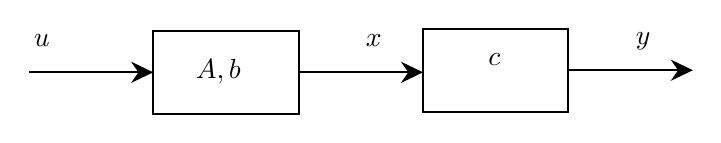
\begin{tikzpicture}[x=0.75pt,y=0.75pt,yscale=-1,xscale=1]
		%uncomment if require: \path (0,59); %set diagram left start at 0, and has height of 59
		
		%Shape: Rectangle [id:dp4470211347634139] 
		\draw   (150,10) -- (220,10) -- (220,50) -- (150,50) -- cycle ;
		\draw    (90,30) -- (147,30) ;
		\draw [shift={(150,30)}, rotate = 180] [fill={rgb, 255:red, 0; green, 0; blue, 0 }  ][line width=0.08]  [draw opacity=0] (10.72,-5.15) -- (0,0) -- (10.72,5.15) -- (7.12,0) -- cycle    ;
		\draw    (220,30) -- (277,30) ;
		\draw [shift={(280,30)}, rotate = 180] [fill={rgb, 255:red, 0; green, 0; blue, 0 }  ][line width=0.08]  [draw opacity=0] (10.72,-5.15) -- (0,0) -- (10.72,5.15) -- (7.12,0) -- cycle    ;
		%Shape: Rectangle [id:dp6612594452533773] 
		\draw   (280,9) -- (350,9) -- (350,49) -- (280,49) -- cycle ;
		\draw    (350,29) -- (407,29) ;
		\draw [shift={(410,29)}, rotate = 180] [fill={rgb, 255:red, 0; green, 0; blue, 0 }  ][line width=0.08]  [draw opacity=0] (10.72,-5.15) -- (0,0) -- (10.72,5.15) -- (7.12,0) -- cycle    ;
		
		\draw (169,22.4) node [anchor=north west][inner sep=0.75pt]    {$A,b$};
		\draw (91,10.4) node [anchor=north west][inner sep=0.75pt]    {$u$};
		\draw (251,10.4) node [anchor=north west][inner sep=0.75pt]    {$x$};
		\draw (310,19.4) node [anchor=north west][inner sep=0.75pt]    {$c$};
		\draw (381,9.4) node [anchor=north west][inner sep=0.75pt]    {$y$};
		
		
	\end{tikzpicture}
\end{figure}\FloatBarrier

La $y$ consiste in una misurazione, che di solito è costosa e vogliamo farne poche. Sotto certe ipotesi, possiamo \textit{ricostruire} lo stato a partire dall'uscita.

\begin{defn}
	$\tilde{x}$ è uno \textbf{stato non osservabile} in $[ 0,t]$ se lasciando evolvere il sistema di movimento libero, trovo in uscita $y(\tau) =0\ \forall \tau \in [ 0,t]$.
\end{defn}

Chiamiamo \textbf{insieme di non osservabilità}
\begin{equation*}
	X_{NO}(t) =\left\{\tilde{x} :c\phi (\tau)\tilde{x} =0\ \forall \tau \in [ 0,t]\right\} \subseteq \mathbb{R}^n
\end{equation*}
$X_{NO}(t)$ è un sottospazio di $\mathbb{R}^n$.

Se $t_2  >t_1 \implies X_{NO}(t_2) \subset X_{NO}(t_1)$. Se l'uscita è nulla in $[ 0,t_2]$, allora lo è anche in $[ 0,t_1]$. Al passare del tempo tende a diventare più piccolo, con discontinuità perché è un sottospazio. Definiamo $t^{*}$ l'ultimo istante in cui non cambia $X_{NO}$, cioè
\begin{equation*}
	X_{NO}(t) =X_{NO}\left(t^{*}\right) \ \forall t\geq t^{*}
\end{equation*}
Questo spazio $X_{NO}\left(t^{*}\right)$ lo chiamiamo semplicemente \textbf{sottospazio di non osservabilità}.
\begin{defn}
	$(A,c)$ è completamente osservabile se $X_{NO} =\{0\}$, ovvero $\dim X_{NO} =0$.
\end{defn}
Introduciamo la \textbf{matrice di osservabilità} $O$
\begin{equation*}
	\boxed{O=\begin{bmatrix}
		c\\
		cA\\
		\vdots \\
		cA^{n-1}
		\end{bmatrix} \in \mathbb{R}^{n\times n}
	}
\end{equation*}
Si dimostra che
\begin{equation*}
	X_{NO} =\ker(O) =\left[\Im\left(O^T\right)\right]^{\perp }
\end{equation*}
da cui si deduce anche
\begin{equation*}
	\dim(X_{NO}) =\dim(\ker(O)) =n-\rank(O)
\end{equation*}
e che
\begin{equation*}
	(A,b) \ \text{compl. oss.} \ \ \iff \ \ \rank(O) =n\ \ \iff \ \ \det O\neq 0
\end{equation*}
\textit{Dimostrazione a tempo discreto (perché più facile).}

Ribadiamo che consideriamo il movimento libero, ovvero $u=0$, ovvero $x(t+1) =Ax(t) +\cancel{bu(t)}$ e misuriamo $y(t) =cx(t)$
\begin{equation*}
	\begin{aligned}
		x(0)   & =\tilde{x}    & y(0) =c\tilde{x}    \\
		x(1)   & =A\tilde{x}   & y(1) =cA\tilde{x}   \\
		\vdots &               & \vdots              \\
		x(t)   & =A^t\tilde{x} & y(t) =cA^t\tilde{x} 
	\end{aligned}
\end{equation*}
Possiamo riscrivere le uscite come
\begin{equation*}
	\begin{bmatrix}
		y(0)   \\
		y(1)   \\
		\vdots \\
		y(t)   
	\end{bmatrix} =\begin{bmatrix}
	c\\
	cA\\
	\vdots \\
	cA^t
	\end{bmatrix}\tilde{x}
\end{equation*}
Gli stati $\tilde{x}$ che danno luogo a $y=0$, ovvero sono tutti e soli gli $\tilde{x}$ che compongono lo spazio nullo di quella matrice, cioè il suo nucleo. Mi fermo a $cA^{n-1}$ per il discorso fatto per la raggiungibilità con il teorema di Cayley-Hamilton.

\section{Ricostruzione dello stato}

Chiamiamo $\hat{x}(t)$ la nostra ricostruzione dello stato. Se $\Sigma $ è il processo/impianto originale, diciamo che $\hat{\Sigma }$ è un ricostruttore asintotico di $\Sigma $ se
\begin{equation*}
	(\hat{x}(t) -x(t))\xrightarrow{t\to \infty } 0\ \ \forall \hat{x}(0) ,x(0)
\end{equation*}

\begin{figure}[htpb]\centering
	\tikzset{every picture/.style={line width=0.75pt}} %set default line width to 0.75pt        
	
	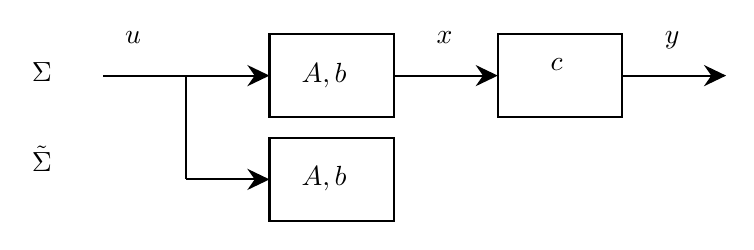
\begin{tikzpicture}[x=0.75pt,y=0.75pt,yscale=-1,xscale=1]
		%uncomment if require: \path (0,116); %set diagram left start at 0, and has height of 116
		
		%Shape: Rectangle [id:dp530061199877327] 
		\draw   (170,15) -- (230,15) -- (230,55) -- (170,55) -- cycle ;
		%Shape: Rectangle [id:dp3924743952847387] 
		\draw   (280,15) -- (340,15) -- (340,55) -- (280,55) -- cycle ;
		%Shape: Rectangle [id:dp7313029033167311] 
		\draw   (170,65) -- (230,65) -- (230,105) -- (170,105) -- cycle ;
		\draw    (90,35) -- (167,35) ;
		\draw [shift={(170,35)}, rotate = 180] [fill={rgb, 255:red, 0; green, 0; blue, 0 }  ][line width=0.08]  [draw opacity=0] (10.72,-5.15) -- (0,0) -- (10.72,5.15) -- (7.12,0) -- cycle    ;
		\draw    (130,85) -- (167,85) ;
		\draw [shift={(170,85)}, rotate = 180] [fill={rgb, 255:red, 0; green, 0; blue, 0 }  ][line width=0.08]  [draw opacity=0] (10.72,-5.15) -- (0,0) -- (10.72,5.15) -- (7.12,0) -- cycle    ;
		\draw    (130,35) -- (130,85) ;
		\draw    (230,35) -- (277,35) ;
		\draw [shift={(280,35)}, rotate = 180] [fill={rgb, 255:red, 0; green, 0; blue, 0 }  ][line width=0.08]  [draw opacity=0] (10.72,-5.15) -- (0,0) -- (10.72,5.15) -- (7.12,0) -- cycle    ;
		\draw    (340,35) -- (387,35) ;
		\draw [shift={(390,35)}, rotate = 180] [fill={rgb, 255:red, 0; green, 0; blue, 0 }  ][line width=0.08]  [draw opacity=0] (10.72,-5.15) -- (0,0) -- (10.72,5.15) -- (7.12,0) -- cycle    ;
		
		\draw (54,27.4) node [anchor=north west][inner sep=0.75pt]    {$\Sigma $};
		\draw (54,67.4) node [anchor=north west][inner sep=0.75pt]    {$\tilde{\Sigma }$};
		\draw (99,12.4) node [anchor=north west][inner sep=0.75pt]    {$u$};
		\draw (184,27.4) node [anchor=north west][inner sep=0.75pt]    {$A,b$};
		\draw (184,77.4) node [anchor=north west][inner sep=0.75pt]    {$A,b$};
		\draw (249,12.4) node [anchor=north west][inner sep=0.75pt]    {$x$};
		\draw (359,12.4) node [anchor=north west][inner sep=0.75pt]    {$y$};
		\draw (304,25.4) node [anchor=north west][inner sep=0.75pt]    {$c$};
		
		
	\end{tikzpicture}
\end{figure}\FloatBarrier

Questi due sistemi sono descritti da
\begin{gather*}
	\dot{x} =Ax+bu\\
	\dot{\hat{x}} =A\hat{x} +bu
\end{gather*}
facciamo la differenza e definiamo un errore
\begin{equation*}
	\underbrace{\dot{\hat{x}} -\dot{x}}_{\dot{e}(t)} =A\underbrace{(\hat{x} -x)}_{e(t)} \ \ \implies \ \ \dot{e}(t) =Ae(t)
\end{equation*}
L'errore che vorremmo far tendere a $0$ è governato dalla matrice $A$. Se $A$ è asint. stabile, $e(t)\to 0\ \forall e(0)$ e cioè $\hat{x}(t)\to x(t) \ \forall \hat{x}(0) ,x(0)$, che è il requisito affinché $\tilde{\Sigma }$ sia un ricostruttore asintotico. Non ci soddisfa perché non tutti i sistemi sono asint. stabili e il tempo che ci mette ad andare a regime è governato sempre dal sistema $A$. L'approccio giusto è sfruttare l'informazione dell'uscita.

\begin{figure}[htpb]\centering
	\tikzset{every picture/.style={line width=0.75pt}} %set default line width to 0.75pt        
	
	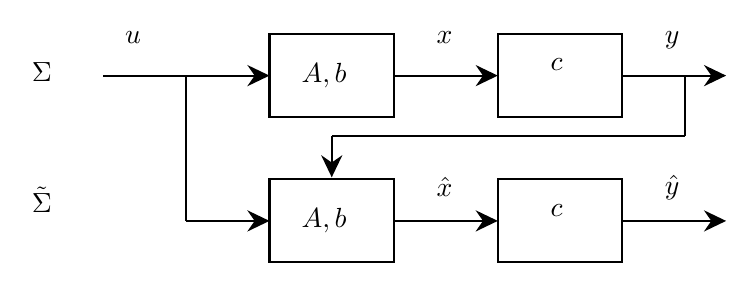
\begin{tikzpicture}[x=0.75pt,y=0.75pt,yscale=-1,xscale=1]
		%uncomment if require: \path (0,143); %set diagram left start at 0, and has height of 143
		
		%Shape: Rectangle [id:dp5226103116096039] 
		\draw   (170,21) -- (230,21) -- (230,61) -- (170,61) -- cycle ;
		%Shape: Rectangle [id:dp9751405884611399] 
		\draw   (280,21) -- (340,21) -- (340,61) -- (280,61) -- cycle ;
		%Shape: Rectangle [id:dp45296026003427614] 
		\draw   (170,91) -- (230,91) -- (230,131) -- (170,131) -- cycle ;
		\draw    (90,41) -- (167,41) ;
		\draw [shift={(170,41)}, rotate = 180] [fill={rgb, 255:red, 0; green, 0; blue, 0 }  ][line width=0.08]  [draw opacity=0] (10.72,-5.15) -- (0,0) -- (10.72,5.15) -- (7.12,0) -- cycle    ;
		\draw    (130,111) -- (167,111) ;
		\draw [shift={(170,111)}, rotate = 180] [fill={rgb, 255:red, 0; green, 0; blue, 0 }  ][line width=0.08]  [draw opacity=0] (10.72,-5.15) -- (0,0) -- (10.72,5.15) -- (7.12,0) -- cycle    ;
		\draw    (130,41) -- (130,111) ;
		\draw    (230,41) -- (277,41) ;
		\draw [shift={(280,41)}, rotate = 180] [fill={rgb, 255:red, 0; green, 0; blue, 0 }  ][line width=0.08]  [draw opacity=0] (10.72,-5.15) -- (0,0) -- (10.72,5.15) -- (7.12,0) -- cycle    ;
		\draw    (340,41) -- (387,41) ;
		\draw [shift={(390,41)}, rotate = 180] [fill={rgb, 255:red, 0; green, 0; blue, 0 }  ][line width=0.08]  [draw opacity=0] (10.72,-5.15) -- (0,0) -- (10.72,5.15) -- (7.12,0) -- cycle    ;
		\draw    (370,41) -- (370,70) ;
		\draw    (370,70) -- (200,70) ;
		\draw    (200,70) -- (200,87) ;
		\draw [shift={(200,90)}, rotate = 270] [fill={rgb, 255:red, 0; green, 0; blue, 0 }  ][line width=0.08]  [draw opacity=0] (10.72,-5.15) -- (0,0) -- (10.72,5.15) -- (7.12,0) -- cycle    ;
		\draw    (230,111) -- (277,111) ;
		\draw [shift={(280,111)}, rotate = 180] [fill={rgb, 255:red, 0; green, 0; blue, 0 }  ][line width=0.08]  [draw opacity=0] (10.72,-5.15) -- (0,0) -- (10.72,5.15) -- (7.12,0) -- cycle    ;
		%Shape: Rectangle [id:dp02965680067021048] 
		\draw   (280,91) -- (340,91) -- (340,131) -- (280,131) -- cycle ;
		\draw    (340,111) -- (387,111) ;
		\draw [shift={(390,111)}, rotate = 180] [fill={rgb, 255:red, 0; green, 0; blue, 0 }  ][line width=0.08]  [draw opacity=0] (10.72,-5.15) -- (0,0) -- (10.72,5.15) -- (7.12,0) -- cycle    ;
		
		\draw (54,33.4) node [anchor=north west][inner sep=0.75pt]    {$\Sigma $};
		\draw (54,93.4) node [anchor=north west][inner sep=0.75pt]    {$\tilde{\Sigma }$};
		\draw (99,18.4) node [anchor=north west][inner sep=0.75pt]    {$u$};
		\draw (184,33.4) node [anchor=north west][inner sep=0.75pt]    {$A,b$};
		\draw (184,103.4) node [anchor=north west][inner sep=0.75pt]    {$A,b$};
		\draw (249,18.4) node [anchor=north west][inner sep=0.75pt]    {$x$};
		\draw (359,18.4) node [anchor=north west][inner sep=0.75pt]    {$y$};
		\draw (304,31.4) node [anchor=north west][inner sep=0.75pt]    {$c$};
		\draw (249,88.4) node [anchor=north west][inner sep=0.75pt]    {$\hat{x}$};
		\draw (359,87.4) node [anchor=north west][inner sep=0.75pt]    {$\hat{y}$};
		\draw (304,101.4) node [anchor=north west][inner sep=0.75pt]    {$c$};
		
		
	\end{tikzpicture}
\end{figure}\FloatBarrier

L'impianto $\Sigma $ funziona così
\begin{gather*}
	\dot{x} =Ax+bu\\
	y=cx
\end{gather*}
Proponiamo un ricostruttore fatto così
\begin{gather*}
	\boxed{\dot{\hat{x}} =A\hat{x} +bu+l(\hat{y} -y)}\\
	\hat{y} =c\hat{x}
\end{gather*}
$\hat{y}$ è l'uscita stimata, quella genererebbe lo stimatore attraverso un'equazione di uscita identica a quella dell'impianto. Come prima possiamo trovare come evolve l'errore
\begin{gather*}
	\begin{aligned}
		\dot{e} =\dot{\hat{x}} -\dot{x} & =A\hat{x} +\cancel{bu} +l(\hat{y} -y) -\left[ Ax+\cancel{bu}\right] \\
		                                & =A(\hat{x} -x) +l(\hat{y} -y)                                       \\
		                                & =Ae+l\left(c\tilde{x} -cx\right)                                    \\
		                                & =Ae+lc\left(\tilde{x} -x\right)                                     \\
		                                & =Ae+lce                                                             \\
		                                & =(A+lc) e                                                           
	\end{aligned}\\
	\Downarrow \\
	\boxed{\dot{e}(t) =(A+lc) e(t)}
\end{gather*}
con
\begin{equation*}
	l=\begin{bmatrix}
	l_1\\
	\vdots \\
	l_n
	\end{bmatrix}
\end{equation*}
\begin{thm}
	Teorema di assegnamento degli autovalori. Per ogni polinomio $\Delta ^{*}(\lambda) =\lambda ^n +\alpha ^{*}_1 \lambda ^{n-1} +\cdots +\alpha ^{*}_n$ esiste $l$ tale che $\Delta _{A+lc}(\lambda) =\Delta ^{*}(\lambda)$, se e solo se $(A,c)$ è completamente osservabile.
\end{thm}

Se inoltre $c$ è un vettore riga (l'uscita è scalare), $l$ è unico.

\section{Scomposizione in parte osservabile e non osservabile}

Studiamo il caso di non completa osservabilità, cioè $\rank(O) =o< n$. Definiamo $X_O$ \textbf{sottospazio di osservabilità}
\begin{equation*}
	X_O =X^{\perp }_{NO} \ \ \implies \ \ \dim X_O =\rank(O) =o
\end{equation*}
è il complemento ortogonale di $X_{NO}$. Qualunque sistema non completamente osservabile si scompone in $2$ sistemi di cui uno compl. oss. e uno non compl. oss. Questa scomposizione si vede facendo un cambio di coordinate, che esiste sempre:
\begin{equation*}
	z=Tx
\end{equation*}
Il nuovo vettore di stato $z$ lo potremo sempre vedere come
\begin{equation*}
	z=\begin{bmatrix}
	z_O\\
	z_{NO}
	\end{bmatrix}
\end{equation*}
Gli stati non osservabili sono del tipo del tipo $z=\begin{bmatrix}
0\\
z_{NO}
\end{bmatrix}$

Il cambio di coordinate permette di guardare $A$ e $b$ in modo diverso:
\begin{equation*}
	(A,b)\implies \left(\underbrace{TAT^{-1}}_{\tilde{A}} ,\underbrace{Tb}_{\tilde{b}} ,\underbrace{cT^{-1}}_{\tilde{c}}\right)
\end{equation*}
Algebricamente
\begin{equation*}
	\tilde{A} =\begin{bmatrix}
	A_O & 0\\
	A_{O,NO} & A_{NO}
	\end{bmatrix} \ \ \ \ \tilde{c} =\begin{bmatrix}
	c_O & 0
	\end{bmatrix}
\end{equation*}
Dove $A_O ,c_O$ è un sistema completamente osservabile.
\begin{defn}
	$(A,c)$ si dice rivelabile se $\exists l$ tale che $(A+lc)$ è asint. stabile, cioè se ammette un ricostruttore asintotico.
\end{defn}
Segue quindi che
\begin{itemize}
	\item se $(A,c)$ è completamente osservabile, allora è rivelabile
	\item se $(A,b)$ non è completamente osservabile, si induce la scomposizione e vuol dire che possiamo assegnare liberamente solo gli autovalori della parte osservabile. Pertanto è rivelabile se e solo se $A_{NO}$ è di suo asint. stabile.
\end{itemize}

\chapter{Teorema di separazione e sintesi del regolatore}

Legge di controllo + ricostruttore dello stato.

\begin{figure}[htpb]\centering
	\tikzset{every picture/.style={line width=0.75pt}} %set default line width to 0.75pt        
	
	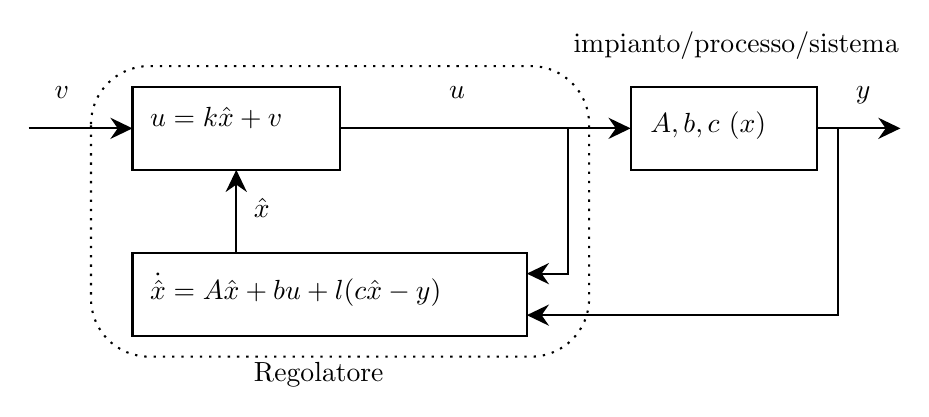
\begin{tikzpicture}[x=0.75pt,y=0.75pt,yscale=-1,xscale=1]
		%uncomment if require: \path (0,200); %set diagram left start at 0, and has height of 200
		
		%Shape: Rectangle [id:dp7056861350500749] 
		\draw   (90,40) -- (190,40) -- (190,80) -- (90,80) -- cycle ;
		\draw    (40,60) -- (87,60) ;
		\draw [shift={(90,60)}, rotate = 180] [fill={rgb, 255:red, 0; green, 0; blue, 0 }  ][line width=0.08]  [draw opacity=0] (10.72,-5.15) -- (0,0) -- (10.72,5.15) -- (7.12,0) -- cycle    ;
		\draw    (190,60) -- (327,60) ;
		\draw [shift={(330,60)}, rotate = 180] [fill={rgb, 255:red, 0; green, 0; blue, 0 }  ][line width=0.08]  [draw opacity=0] (10.72,-5.15) -- (0,0) -- (10.72,5.15) -- (7.12,0) -- cycle    ;
		%Shape: Rectangle [id:dp508570979902413] 
		\draw   (90,120) -- (280,120) -- (280,160) -- (90,160) -- cycle ;
		\draw    (140,120) -- (140,83) ;
		\draw [shift={(140,80)}, rotate = 450] [fill={rgb, 255:red, 0; green, 0; blue, 0 }  ][line width=0.08]  [draw opacity=0] (10.72,-5.15) -- (0,0) -- (10.72,5.15) -- (7.12,0) -- cycle    ;
		\draw    (300,60) -- (300,130) -- (283,130) ;
		\draw [shift={(280,130)}, rotate = 360] [fill={rgb, 255:red, 0; green, 0; blue, 0 }  ][line width=0.08]  [draw opacity=0] (10.72,-5.15) -- (0,0) -- (10.72,5.15) -- (7.12,0) -- cycle    ;
		\draw    (430,60) -- (430,150) -- (283,150) ;
		\draw [shift={(280,150)}, rotate = 360] [fill={rgb, 255:red, 0; green, 0; blue, 0 }  ][line width=0.08]  [draw opacity=0] (10.72,-5.15) -- (0,0) -- (10.72,5.15) -- (7.12,0) -- cycle    ;
		%Shape: Rectangle [id:dp8170288028933135] 
		\draw   (330,40) -- (420,40) -- (420,80) -- (330,80) -- cycle ;
		\draw    (420,60) -- (457,60) ;
		\draw [shift={(460,60)}, rotate = 180] [fill={rgb, 255:red, 0; green, 0; blue, 0 }  ][line width=0.08]  [draw opacity=0] (10.72,-5.15) -- (0,0) -- (10.72,5.15) -- (7.12,0) -- cycle    ;
		%Rounded Rect [id:dp9784630292921757] 
		\draw  [color={rgb, 255:red, 0; green, 0; blue, 0 }  ,draw opacity=1 ][dash pattern={on 0.84pt off 2.51pt}] (70,58) .. controls (70,42.54) and (82.54,30) .. (98,30) -- (282,30) .. controls (297.46,30) and (310,42.54) .. (310,58) -- (310,142) .. controls (310,157.46) and (297.46,170) .. (282,170) -- (98,170) .. controls (82.54,170) and (70,157.46) .. (70,142) -- cycle ;
		
		\draw (97,48.4) node [anchor=north west][inner sep=0.75pt]    {$u=k\hat{x} +v$};
		\draw (51,38.4) node [anchor=north west][inner sep=0.75pt]    {$v$};
		\draw (97,128.4) node [anchor=north west][inner sep=0.75pt]    {$\dot{\hat{x}} =A\hat{x} +bu+l(c\hat{x} -y)$};
		\draw (147,92.4) node [anchor=north west][inner sep=0.75pt]    {$\hat{x}$};
		\draw (241,38.4) node [anchor=north west][inner sep=0.75pt]    {$u$};
		\draw (338,50.4) node [anchor=north west][inner sep=0.75pt]    {$A,b,c\ (x)$};
		\draw (301,12) node [anchor=north west][inner sep=0.75pt]   [align=left] {impianto/processo/sistema};
		\draw (437,38.4) node [anchor=north west][inner sep=0.75pt]    {$y$};
		\draw (147,171) node [anchor=north west][inner sep=0.75pt]   [align=left] {Regolatore};
		
		
	\end{tikzpicture}
\end{figure}\FloatBarrier

Complessivamente ha $2n$ variabili di stato
\begin{equation*}
	\begin{bmatrix}
		x       \\
		\hat{x} 
	\end{bmatrix}
\end{equation*}
Da cosa è governato?
\begin{equation*}
	\begin{aligned}
		\begin{bmatrix}
		\dot{x}\\
		\dot{\hat{x}}
		\end{bmatrix} & =\begin{bmatrix}             
		Ax+bu\\
		A\hat{x} +bu+l(c\hat{x} -cx)
		\end{bmatrix}\\
		              & =\begin{bmatrix}             
		Ax+bk\hat{x} +bv\\
		A\hat{x} +bk\hat{x} +bv+lc\hat{x} -lcx
		\end{bmatrix}\\
		              & =\underbrace{\begin{bmatrix} 
		A             & bk                           \\
		-lc           & A+bk+lc                      
		\end{bmatrix}
		}_{A_{\text{reg}}}\begin{bmatrix}
		x\\
		\hat{x}
		\end{bmatrix} +\underbrace{\begin{bmatrix}
		b\\
		b
		\end{bmatrix}
		}_{b_{\text{reg}}} v
	\end{aligned}
\end{equation*}
In questo modo non ha nessuna struttura comoda che ci dice come sia la sua struttura spettrale. Facciamo un cambio di coordinate per svelare la verità
\begin{equation*}
	\begin{bmatrix}
		x          \\
		\hat{x} -x 
	\end{bmatrix} =\begin{bmatrix}
	x\\
	e
	\end{bmatrix} =\begin{bmatrix}
	I & 0\\
	-I & I
	\end{bmatrix}\begin{bmatrix}
	x\\
	\hat{x}
	\end{bmatrix} =T\begin{bmatrix}
	x\\
	\hat{x}
	\end{bmatrix}
\end{equation*}
Quindi $\tilde{A}_{\text{reg}} =TA_{\text{reg}} T^{-1}$
\begin{equation*}
	\begin{bmatrix}
		I  & 0 \\
		-I & I 
	\end{bmatrix}\begin{bmatrix}
	A & bk\\
	-lc & A+bk+lc
	\end{bmatrix}\begin{bmatrix}
	I & 0\\
	I & I
	\end{bmatrix} =\dotsc =\begin{bmatrix}
	A+bk & bk\\
	0 & A+lc
	\end{bmatrix}
\end{equation*}
Miracolo, capiamo la struttura spettrale perché è triangolare a blocchi
\begin{equation*}
	\sigma \left(\tilde{A}_{\text{reg}}\right) =\sigma (A+bk) \cup \sigma (A+lc)
\end{equation*}
Questo si chiama \textbf{Teorema di Separazione}: se e solo se il sistema è compl. oss. e compl. ragg. possiamo progettare gli autovalori di entrambi questi blocchi \textbf{separatamente}, e lo spettro complessivo sarà l'unione degli spettri di questi due sistemi.

Vediamo ora la scomposizione in $4$ parti, o \textbf{scomposizione di Kalman}.

\begin{figure}[htpb]\centering
	\tikzset{every picture/.style={line width=0.75pt}} %set default line width to 0.75pt        
	
	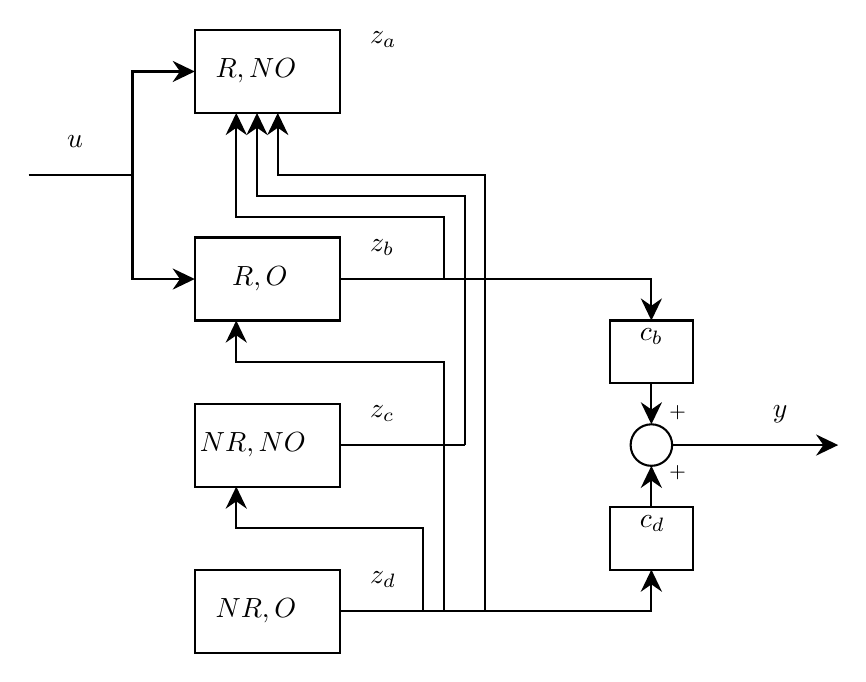
\begin{tikzpicture}[x=0.75pt,y=0.75pt,yscale=-1,xscale=1]
		%uncomment if require: \path (0,319); %set diagram left start at 0, and has height of 319
		
		%Shape: Rectangle [id:dp8477513863321651] 
		\draw   (120,10) -- (190,10) -- (190,50) -- (120,50) -- cycle ;
		\draw    (40,80) -- (90,80) ;
		\draw    (117,30) -- (90,30) -- (90,130) -- (117,130) ;
		\draw [shift={(120,130)}, rotate = 180] [fill={rgb, 255:red, 0; green, 0; blue, 0 }  ][line width=0.08]  [draw opacity=0] (10.72,-5.15) -- (0,0) -- (10.72,5.15) -- (7.12,0) -- cycle    ;
		\draw [shift={(120,30)}, rotate = 180] [fill={rgb, 255:red, 0; green, 0; blue, 0 }  ][line width=0.08]  [draw opacity=0] (10.72,-5.15) -- (0,0) -- (10.72,5.15) -- (7.12,0) -- cycle    ;
		\draw    (240,130) -- (240,100) -- (140,100) -- (140,53) ;
		\draw [shift={(140,50)}, rotate = 450] [fill={rgb, 255:red, 0; green, 0; blue, 0 }  ][line width=0.08]  [draw opacity=0] (10.72,-5.15) -- (0,0) -- (10.72,5.15) -- (7.12,0) -- cycle    ;
		\draw    (190,130) -- (340,130) -- (340,147) ;
		\draw [shift={(340,150)}, rotate = 270] [fill={rgb, 255:red, 0; green, 0; blue, 0 }  ][line width=0.08]  [draw opacity=0] (10.72,-5.15) -- (0,0) -- (10.72,5.15) -- (7.12,0) -- cycle    ;
		%Shape: Rectangle [id:dp12976064727081904] 
		\draw   (120,110) -- (190,110) -- (190,150) -- (120,150) -- cycle ;
		%Shape: Rectangle [id:dp15936028487027354] 
		\draw   (120,190) -- (190,190) -- (190,230) -- (120,230) -- cycle ;
		%Shape: Rectangle [id:dp6195977072835361] 
		\draw   (120,270) -- (190,270) -- (190,310) -- (120,310) -- cycle ;
		\draw    (250,210) -- (250,90) -- (150,90) -- (150,53) ;
		\draw [shift={(150,50)}, rotate = 450] [fill={rgb, 255:red, 0; green, 0; blue, 0 }  ][line width=0.08]  [draw opacity=0] (10.72,-5.15) -- (0,0) -- (10.72,5.15) -- (7.12,0) -- cycle    ;
		\draw    (260,290) -- (260,80) -- (160,80) -- (160,53) ;
		\draw [shift={(160,50)}, rotate = 450] [fill={rgb, 255:red, 0; green, 0; blue, 0 }  ][line width=0.08]  [draw opacity=0] (10.72,-5.15) -- (0,0) -- (10.72,5.15) -- (7.12,0) -- cycle    ;
		%Shape: Circle [id:dp24065301031563058] 
		\draw   (330,210) .. controls (330,204.48) and (334.48,200) .. (340,200) .. controls (345.52,200) and (350,204.48) .. (350,210) .. controls (350,215.52) and (345.52,220) .. (340,220) .. controls (334.48,220) and (330,215.52) .. (330,210) -- cycle ;
		\draw    (190,210) -- (250,210) ;
		\draw    (190,290) -- (340,290) -- (340,273) ;
		\draw [shift={(340,270)}, rotate = 450] [fill={rgb, 255:red, 0; green, 0; blue, 0 }  ][line width=0.08]  [draw opacity=0] (10.72,-5.15) -- (0,0) -- (10.72,5.15) -- (7.12,0) -- cycle    ;
		%Shape: Rectangle [id:dp8069842788370218] 
		\draw   (320,150) -- (360,150) -- (360,180) -- (320,180) -- cycle ;
		%Shape: Rectangle [id:dp8692451305031148] 
		\draw   (320,240) -- (360,240) -- (360,270) -- (320,270) -- cycle ;
		\draw    (230,290) -- (230,250) -- (140,250) -- (140,233) ;
		\draw [shift={(140,230)}, rotate = 450] [fill={rgb, 255:red, 0; green, 0; blue, 0 }  ][line width=0.08]  [draw opacity=0] (10.72,-5.15) -- (0,0) -- (10.72,5.15) -- (7.12,0) -- cycle    ;
		\draw    (240,290) -- (240,170) -- (140,170) -- (140,153) ;
		\draw [shift={(140,150)}, rotate = 450] [fill={rgb, 255:red, 0; green, 0; blue, 0 }  ][line width=0.08]  [draw opacity=0] (10.72,-5.15) -- (0,0) -- (10.72,5.15) -- (7.12,0) -- cycle    ;
		\draw    (340,197) -- (340,180) ;
		\draw [shift={(340,200)}, rotate = 270] [fill={rgb, 255:red, 0; green, 0; blue, 0 }  ][line width=0.08]  [draw opacity=0] (10.72,-5.15) -- (0,0) -- (10.72,5.15) -- (7.12,0) -- cycle    ;
		\draw    (340,240) -- (340,223) ;
		\draw [shift={(340,220)}, rotate = 450] [fill={rgb, 255:red, 0; green, 0; blue, 0 }  ][line width=0.08]  [draw opacity=0] (10.72,-5.15) -- (0,0) -- (10.72,5.15) -- (7.12,0) -- cycle    ;
		\draw    (350,210) -- (427,210) ;
		\draw [shift={(430,210)}, rotate = 180] [fill={rgb, 255:red, 0; green, 0; blue, 0 }  ][line width=0.08]  [draw opacity=0] (10.72,-5.15) -- (0,0) -- (10.72,5.15) -- (7.12,0) -- cycle    ;
		
		\draw (128.5,22.4) node [anchor=north west][inner sep=0.75pt]    {$R,NO$};
		\draw (57,59.4) node [anchor=north west][inner sep=0.75pt]    {$u$};
		\draw (136.5,122.4) node [anchor=north west][inner sep=0.75pt]    {$R,O$};
		\draw (121,202.4) node [anchor=north west][inner sep=0.75pt]    {$NR,NO$};
		\draw (128.5,282.4) node [anchor=north west][inner sep=0.75pt]    {$NR,O$};
		\draw (333,152.4) node [anchor=north west][inner sep=0.75pt]    {$c_b$};
		\draw (203,109.4) node [anchor=north west][inner sep=0.75pt]    {$z_b$};
		\draw (203,189.4) node [anchor=north west][inner sep=0.75pt]    {$z_c$};
		\draw (203,269.4) node [anchor=north west][inner sep=0.75pt]    {$z_d$};
		\draw (203,9.4) node [anchor=north west][inner sep=0.75pt]    {$z_a$};
		\draw (333,242.4) node [anchor=north west][inner sep=0.75pt]    {$c_d$};
		\draw (347,189.4) node [anchor=north west][inner sep=0.75pt]  [font=\scriptsize]  {$+$};
		\draw (347,218.4) node [anchor=north west][inner sep=0.75pt]  [font=\scriptsize]  {$+$};
		\draw (397,189.4) node [anchor=north west][inner sep=0.75pt]    {$y$};
		
		
	\end{tikzpicture}
\end{figure}\FloatBarrier

Ci dice che partendo da un certo $(A,b,c)$ e con una trasformazione $z=Tx$ lo possiamo scomporre in $4$ sottosistemi, $(R,NO) ,(R,O) ,(NR,NO) ,(NR,O)$, e scrivere $z$ come
\begin{equation*}
	z=\begin{bmatrix}
	z_a\\
	z_b\\
	z_c\\
	z_d
	\end{bmatrix} \in \mathbb{R}^n
\end{equation*}
E le altre matrici
\begin{equation*}
	\tilde{A} =\begin{bmatrix}
	A_a & A_{ab} & A_{ac} & A_{ad}\\
	0 & A_b & 0 & A_{bd}\\
	0 & 0 & A_c & A_{cd}\\
	0 & 0 & 0 & A_d
	\end{bmatrix} \ \ \ \ \tilde{b} =\begin{bmatrix}
	b_a\\
	b_b\\
	0\\
	0
	\end{bmatrix} \ \ \ \ \tilde{c} =\begin{bmatrix}
	0 & c_b & 0 & c_d
	\end{bmatrix}
\end{equation*}
Questa coppia è compl. ragg.
\begin{equation*}
	\left(\begin{bmatrix}
	A_a & A_{ab}\\
	0 & A_b
	\end{bmatrix} ,\begin{bmatrix}
	b_a\\
	b_b
	\end{bmatrix} ,-\right)
\end{equation*}
Questa coppia è compl. oss.
\begin{equation*}
	\left(\begin{bmatrix}
	A_b & A_{bd}\\
	0 & A_d
	\end{bmatrix} ,-,\begin{bmatrix}
	c_b & c_d
	\end{bmatrix}\right)
\end{equation*}
Questo blocco è compl. ragg. e compl. oss
\begin{equation*}
	(A_b ,b_b ,c_b)
\end{equation*}
La funzione di trasferimento descrive solo la parte $b$
\begin{equation*}
	G(s) =c(sI-A)^{-1} b=c_b(sI-A_b)^{-1} b_b =G_b(s)
\end{equation*}
Quindi concludiamo che non perde di grado se e solo se il sistema è compl. oss. e compl. ragg. In caso contrario, gli $n$ autovalori della matrice $A$ si distribuiscono tra i vari sottosistemi.

\chapter{Stabilità esterna}

La stabilità interna è quella che abbiamo descritto come $\phi (t) x(0)\to 0\ \forall x(0)$.
\begin{defn}
	$(A,b,c)$ è \textbf{esternamente stabile} se l'uscita forzata $y_{\text{for}}(t)$ è limitata $\forall u(t)$ limitato.
\end{defn}
C'è un'ipotesi di stato iniziale nullo $x(0) =0$. Il movimento forzato lo scriviamo come $x_F(t) =\psi (t)\left( u_{[ 0,t)}\right)$, quindi l'uscita forzata è $y_{\text{for}}(t) =cx_F(t)$
\begin{thm}
	$(A,b,c)$ esternamente stabile $\iff $ $R,O$ asint. stabile $\iff $ $A_b$ asint. stabile.
\end{thm}
Ma i suoi autovalori sono i poli della funzione di trasferimento.
\begin{equation*}
	A_b \ \text{asint. stabile.} \ \iff \ \begin{cases}
	\Re(p_i) < 0\ \forall i & \text{t.c.}\\
	| p_i| < 1\ \forall i & \text{t.d.}
	\end{cases}
\end{equation*}
Se $A$ è asint. stabile, tutti i suoi autovalori negativi si distribuiscono nelle quattro parti, quindi la funzione di trasferimento avrà poli negativi, $\implies $ $(A,b,c)$ esternamente stabile. Non vale l'opposto in generale, non sappiamo nulla sulle tre parti al di fuori di quella $(O,R)$. Se $(A,b,c)$ è compl. oss. e compl. ragg. vale la coimplicazione
\begin{equation*}
	A\ \text{asint. stabile.} \ \iff \ (A,b,c) \ \text{esternamente stabile}
\end{equation*}
Salvo quasi critici, sono quasi sempre compl. oss. e compl. ragg. Il fatto che l'ingresso non influenzi uno stato e che l'uscita non dipenda da qualcuno di questi, è in qualche modo una cosa anomala.

\chapter{Risposte canoniche}

Studiamo il movimento forzato, ovvero la risposta del sistema a specifici ingressi, impulso, scalino, rampa e sinusoide (risposta in frequenza). Quindi ipotizziamo $x(0) =0$.

\section{Risposta all'impulso (tempo continuo)}

\begin{figure}[htpb]\centering
	\tikzset{every picture/.style={line width=0.75pt}} %set default line width to 0.75pt        
	
	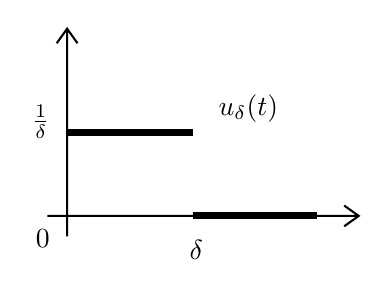
\begin{tikzpicture}[x=0.75pt,y=0.75pt,yscale=-1,xscale=1]
		%uncomment if require: \path (0,134); %set diagram left start at 0, and has height of 134
		
		%Shape: Axis 2D [id:dp3394460818570706] 
		\draw  (110,100.2) -- (260,100.2)(119.5,10) -- (119.5,110) (253,95.2) -- (260,100.2) -- (253,105.2) (114.5,17) -- (119.5,10) -- (124.5,17)  ;
		\draw [line width=2.25]    (120,60) -- (180,60) ;
		\draw [line width=2.25]    (180,100) -- (240,100) ;
		
		\draw (103,105.4) node [anchor=north west][inner sep=0.75pt]    {$0$};
		\draw (101,45.4) node [anchor=north west][inner sep=0.75pt]    {$\frac{1}{\delta }$};
		\draw (177,110.4) node [anchor=north west][inner sep=0.75pt]    {$\delta $};
		\draw (191,40.4) node [anchor=north west][inner sep=0.75pt]    {$u_{\delta }(t)$};
		
		
	\end{tikzpicture}
\end{figure}\FloatBarrier

Si ha $\int ^{+\infty }_0 u_{\delta }(t) dt=1$. Facciamo tendere $\delta \to 0$ e troviamo l'impulso. Ha queste proprietà:
\begin{itemize}
	\item $\imp(t) =0\ \forall t\neq 0$
	\item $\int ^{0^{+}}_{0^{-}}\imp(t) dt=1$
\end{itemize}

Studiamo l'uscita
\begin{equation*}
	\begin{aligned}
		y(t) =cx(t) & =c\int ^t_0 e^{A(t-\tau)} bu(\tau) d\tau                \\
		            & =c\int ^{0^{+}}_{0^{-}} e^{A(t-\tau)} b\imp(\tau) d\tau \\
		            & =ce^{At} b\int ^{0^{+}}_{0^{-}}\imp(\tau) d\tau         \\
		            & =\boxed{ce^{At} b=c\phi (t) b=g(t)}                     
	\end{aligned}
\end{equation*}

\section{Risposta all'impulso (tempo discreto)}

Si definisce come
\begin{equation*}
	\imp(t) =\begin{cases}
	1, & t=0\\
	0, & t >0
	\end{cases}
\end{equation*}
L'uscita all'istante $0$ vale
\begin{equation*}
	y(0) =cx(0) +du(0) =d
\end{equation*}
quindi se il sistema è improprio c'è questa unica differenza. Quindi assumiamo $d=0$, per il resto
\begin{equation*}
	\begin{aligned}
		x(0) & =0                & y(0) =0          \\
		x(1) & =Ax(0) +bu(0) =b  & y(1) =cx(1) =cb  \\
		x(2) & =Ax(1) +bu(1) =Ab & y(2) =cx(2) =cAb 
	\end{aligned}
\end{equation*}
In generale
\begin{equation*}
	\boxed{g(t) =\begin{cases}
		0, & t=0\\
		cA^{t-1} b=c\phi (t-1) b, & t >0
		\end{cases}
	}
\end{equation*}

\section{Trasformata di Laplace}

Notiamo ora che
\begin{equation*}
	\begin{aligned}
		y(t) =cx(t) & =c\int ^t_0 e^{A(t-\tau)} bu(\tau) d\tau         \\
		            & =\int ^t_0\boxed{ce^{A(t-\tau)} b} u(\tau) d\tau \\
		            & =\int ^t_0\boxed{g(t-\tau)} u(\tau) d\tau        
	\end{aligned}
\end{equation*}
è detto \textbf{integrale di convoluzione}
\begin{equation}
	y(t) =g(t) *u(t)
\end{equation}
La trasformata di Laplace è definita come
\begin{equation}
	F(s) :\mathbb{C}\to \mathbb{C} \ \ \ \ F(s) =\mathcal{L} a[ f(t)] =\int ^{+\infty }_0 f(t) e^{-st} dt
\end{equation}
In particolare
\begin{equation*}
	\mathcal{L}^{-1}[\mathcal{L}[ f(t)]] =f(t)
\end{equation*}
Consideriamo ora la trasformata di Laplace di alcuni ingressi $u(t)$ canonici
\begin{itemize}
	\item $u(t) =\imp(t)$, allora\begin{equation*}
	      \begin{aligned}
	      	U(s) & =\int ^{+\infty }_0\imp(t) e^{-st} dt \\
	      	     & =\int ^{0^{+}}_{0^{-}}\imp(t) dt=1    
	      \end{aligned}
	\end{equation*}
	\item $u(t) =\step(t)$, allora\begin{equation*}
	      \begin{aligned}
	      	U(s) & =\int ^{+\infty }_0 1\cdotp e^{-st} dt                                                   \\
	      	     & =-\frac{1}{s}\left[ e^{-st}\right]^{+\infty }_0 =\frac{1}{s} ,\ \ \text{se} \ \Re(s)  >0 
	      \end{aligned}
	\end{equation*}
	\item $f(t) =e^{at} ,a\in \mathbb{R}$, allora\begin{equation*}
	      \begin{aligned}
	      	F(s) & =\int ^{+\infty }_0 e^{at} e^{-st} dt=\int ^{+\infty }_0 e^{(a-s) t} dt \\
	      	     & =\frac{1}{a-s}\left[ e^{(a-s) t}\right]^{+\infty }_0                    \\
	      	     & =\frac{1}{s-a} ,\ \ \text{se} \ \Re(s)  >\Re(a)                         
	      \end{aligned}
	\end{equation*}
	\item $f(t) =te^{at}$, allora $F(s) =\frac{1}{(s-a)^2}$
	\item $f(t) =\frac{1}{2} t^2 e^{at}$, allora $F(s) =\frac{1}{(s-a)^3}$
	\item $u(t) =\ramp(t)$, allora $U(s) =\frac{1}{s^2}$
\end{itemize}

\begin{center}
	
	\begin{tabular}{ccccccc}
		\toprule 
		$u(t)$ & $\imp(t)$ & $\step(t)$     & $e^{at}$        & $te^{at}$           & $\frac{1}{2!} t^2 e^{at}$ & $\ramp(t)$      \\
		\midrule 
		$U(s)$ & $1$       & $\frac{1}{s}$ & $\frac{1}{s-a}$ & $\frac{1}{(s-a)^2}$ & $\frac{1}{(s-a)^3}$       & $\frac{1}{s^2}$ \\
		\bottomrule
	\end{tabular}
\end{center}

La trasformata gode delle seguenti \textbf{proprietà}
\begin{itemize}
	\item \textbf{linearità}, siano $f_1(t)\implies F_1(s) ,f_2(t)\implies F_2(s)$ e siano $\alpha ,\beta \in \mathbb{R}$\begin{equation*}
	      \alpha f_1(t) +\beta f_2(t) \ \ \xrightarrow{\mathcal{L}} \ \ \alpha F_1(s) +\beta F_2(s)
	\end{equation*}
	\item \textbf{derivazione}, sia $f(t)\implies F(s)$\begin{gather*}
	      h(t) =\frac{df(t)}{dt} \ \ \xrightarrow{\mathcal{L}} \ \ H(s) =\mathcal{L}\left[\frac{df(t)}{dt}\right] =sF(s) -f(0)\\
	      \mathcal{L}\left[\frac{d^2 f(t)}{dt^2}\right] =s\mathcal{L}\left[\frac{df(t)}{dt}\right] -f'(0) =s^2 F(s) -sf(0) -f'(0)
	\end{gather*}
	
	il termine $f(0) ,\dotsc $ è quasi sempre $0$ nei nostri casi.
	\item \textbf{integrazione}, sia $f(t)\implies F(s)$\begin{equation*}
	      h(t) =\int ^t_0 f(\tau) d\tau \ \ \xrightarrow{\mathcal{L}} \ \ H(s) =\frac{1}{s} F(s)
	\end{equation*}
	\item \textbf{traslazione}, sia $f(t)\implies F(s)$\begin{equation}
	      h(t) =\begin{cases}
	      0, & 0\leq t< T\\
	      f(t-T) , & t >T
	\end{cases} \ \ \xrightarrow{\mathcal{L}
		} \ \ H(s) =F(s) e^{-sT}
	\end{equation}
	\item \textbf{convoluzione}, siano $f(t)\implies F(s) ,h(t)\implies H(s)$\begin{equation*}
	      f(t) *h(t) =\int ^t_0 f(t-\tau) h(\tau) d\tau \ \ \xrightarrow{\mathcal{L}} \ \ F(s) H(s)
	\end{equation*}
\end{itemize}

Con la trasformata di Laplace (e da qui alla fine del corso) analizzeremo solo sistemi a tempo continuo.

\section{Relazione tra funzione di trasferimento e risposta all'impulso}

Abbiamo visto che la risposta all'impulso $u(t) =\imp(t)$ è $y(t) =ce^{At} b=g(t)$ che ha una sua trasformata di Laplace
\begin{equation*}
	\mathcal{L}[ g(t)] =\mathcal{L}\left[ ce^{At} b\right] =c\mathcal{L}\left[ e^{At}\right] b=c(sI-A)^{-1} b=G(s)
\end{equation*}
La sua funzione di trasferimento è la trasformata di Laplace della risposta all'impulso, ponte importantissimo!

\section{Relazione tra risposta allo scalino e risposta all'impulso}

Si ha che la risposta all'impulso è uguale alla derivata della risposta allo scalino:
\begin{equation*}
	\boxed{y_{\imp}(t) =\frac{d}{dt}[ y_{\step}(t)]}
\end{equation*}

\section{Calcolo di risposte canoniche}

Ricordiamo che l'uscita si può vedere come convoluzione e possiamo passare alle trasformate
\begin{equation*}
	y(t) =\int ^t_0 g(t-\tau) u(\tau) d\tau \xrightarrow{\mathcal{L}}\boxed{Y(s) =G(s) U(s)}
\end{equation*}
Il percorso che dovremmo fare in generale è
\begin{equation*}
	u(t)\xrightarrow{\mathcal{L}} U(s) \ \ \implies \ \ Y(s) =G(s) U(s) \ \ \implies \ \ Y(s)\xrightarrow{\mathcal{L}^{-1}} y(t)
\end{equation*}
In generale le trasformate sono rognose, ma \textbf{se l'ingresso è canonico, la sua trasformata è razionale fratta}. Tutto diventa più facile.

\section{Risposta allo scalino}

\textit{Esempio.} Sia
\begin{equation*}
	G(s) =\frac{2(s-1)}{(s+1)(s+2)^2} \ \ \ \ u(t) =\step(t) \implies U(s) =\frac{1}{s}
\end{equation*}
Introduciamo il \textbf{grado relativo}
\begin{equation*}
	\boxed{r=\#\text{poli} -\#\text{zeri} =\mathrm{deg}(D) -\mathrm{deg}(N)}
\end{equation*}
qui $r=2$. Calcoliamo agevolmente l'uscita
\begin{equation*}
	Y(s) =G(s) U(s) =\frac{2(s-1)}{s(s+1)(s+2)^2}
\end{equation*}
ora dobbiamo antitrasformare, facciamo lo \textbf{sviluppo di Heaviside}. Scomponiamo in tante frazioni quant'è il grado del denominatore.
\begin{equation}
	Y(s)=\frac{A}{s} +\frac{B}{s+1} +\frac{C}{s+2} +\frac{D}{(s+2)^2}
\end{equation}
che è facile da antitrasformare
\begin{equation*}
	\begin{aligned}
		y(t) =\mathcal{L}^{-1}[ Y(s)] & =A\mathcal{L}^{-1}\left[\frac{1}{s}\right] +B\mathcal{L}^{-1}\left[\frac{1}{s+1}\right] +C\mathcal{L}^{-1}\left[\frac{1}{s+2}\right] +D\mathcal{L}^{-1}\left[\frac{1}{(s+2)^2}\right] \\
		                              & =A+Be^{-t} +Ce^{-2t} +Dte^{-2t}                                                                                                                                                       
	\end{aligned}
\end{equation*}
La scomposizione (8) si fa così:
\begin{equation*}
	\frac{A(s+1)(s+2)^2 +Bs(s+2)^2 +Cs(s+1)(s+2)+Ds(s+1)}{s(s+1)(s+2)^2} =\frac{2(s-1)}{s(s+1)(s+2)^2}
\end{equation*}
\begin{itemize}
	\item Se $s=-1\implies -B=-4\implies B=4$.
	\item Se $s=-2\implies 2D=-6\implies D=-3$.
	\item Se $s=0\implies 4A=-2\implies A=-\frac{1}{2}$.
	\item Se $s=1\implies 18A+9B+6C+2D=0\implies C=-\frac{7}{2}$.
\end{itemize}

Si ottiene quindi l'uscita
\begin{equation*}
	y(t)=-\frac{1}{2} +4e^{-t} -\frac{7}{2} e^{-2t} -3te^{-2t}
\end{equation*}
Che si può studiare:
\begin{itemize}
	\item valore iniziale\begin{equation*}
	      y(0) =-\frac{1}{2} +4-\frac{7}{2} =\frac{-1+8-7}{2} =0
	\end{equation*}
	\item valore asintotico\begin{equation*}
	      \lim _{t\to +\infty } y(t) =-\frac{1}{2}
	\end{equation*}
	
	questo risultato lo sapevamo già ($\overline{u} =1$ perché stiamo considerando lo scalino unitario)\begin{equation*}
	\overline{y} =\mu \overline{u} =G(0) \cdotp 1=-\frac{1}{2}
	\end{equation*}
	\item derivata prima\begin{gather*}
	      y'(t) =-4e^{-t} +7e^{-2t} -3\left(e^{-2t} -2te^{-2t}\right) =-4e^{-t} +4e^{-2t} +6te^{-2t}\\
	      \implies y'(0) =-4+4=0
	\end{gather*}
	\item derivata seconda\begin{gather*}
	      y''(t) =4e^{-t} -8e^{-2t} +6\left[ e^{-2t} -2te^{-2t}\right] =4e^{-t} -2e^{-2t} -12te^{-2t}\\
	      \implies y''(0) =4-2=2
	\end{gather*}
\end{itemize}

\textbf{Calcolo qualitativo delle risposte canoniche}
\begin{itemize}
	\item valore finale/asintotico $y(\infty)$
	\item tempo di risposta
	\item valore iniziale $y(0)$
	\item derivate iniziali
	\item estremi (massimi e minimi)
	\item oscillazioni (poli complessi)
\end{itemize}
\begin{thm}{Teorema del valore iniziale.}{}
	Sia $f(t)\xrightarrow{\mathcal{L}} F(s)$ allora
	\begin{equation*}
		\boxed{f(0) =\lim _{t\to 0^{+}} f(t) =\lim _{\Re(s)\to \infty }[ sF(s)]}
	\end{equation*}
\end{thm}
Lo possiamo usare insieme ad altri teoremi, come quello della derivazione
\begin{equation*}
	f'(0) =\lim _{s\to \infty } s\mathcal{L}[ f'(t)] =\lim _{s\to \infty } s(sF(s) -f(0))
\end{equation*}
\begin{thm}{Teorema del valore finale.}{}
	Sia $f(t)\xrightarrow{\mathcal{L}} F(s)$ allora
	\begin{equation*}
		\boxed{\lim _{t\to \infty } f(t) =\lim _{\Re(s)\to 0}[ sF(s)]}
	\end{equation*}
\end{thm}
\textit{Esempio.} Sia $T >0$
\begin{equation*}
	G(s) =\frac{\mu }{1+sT}
\end{equation*}
che è asint. stabile. Il polo è $s=-\frac{1}{T}$, la costante di tempo è
\begin{equation*}
	-\frac{1}{-\frac{1}{T}} =T
\end{equation*}
Invece
\begin{equation*}
	G(0) =\mu 
\end{equation*}
Questo modo mette in evidenza costante di tempo e guadagno. Com'è la risposta allo scalino? Usiamo il teorema del valore iniziale e ricordiamo che con lo scalino si ha $U(s) =\frac{1}{s}$ per ottenere:
\begin{equation*}
	y(0) =\lim _{s\to \infty } sY(s) =\lim _{s\to \infty } sG(s) U(s) =\lim _{s\to \infty } s\frac{\mu }{1+sT}\frac{1}{s} =\lim _{s\to \infty }\frac{\mu }{1+sT} =0
\end{equation*}
Vediamo la derivata prima
\begin{equation*}
	\dot{y}(t) =\lim _{s\to \infty } s\left(sY(s) -\cancel{y(0)}\right) =\lim _{s\to \infty } s^2 Y(s) =\lim _{s\to \infty } s^2\frac{\mu }{1+sT}\frac{1}{s} =\frac{\mu }{T}
\end{equation*}
\textit{Complichiamo:}
\begin{equation*}
	G(s)=\frac{\mu }{(1+sT_1)(1+sT_2)} \ \ 
\end{equation*}
supponiamo $T_1 ,T_2  >0\implies $ è asint. stabile. $r=2$.
\begin{equation*}
	\begin{aligned}
		y(\infty)    & =G(0)\cdot 1=\mu                                                                                                                                                                          \\
		y(0)         & =\lim _{s\to \infty } sY(s)                                                                                                                                                       \\
		             & =\lim _{s\to \infty } s\frac{1}{s}\frac{\mu }{(1+sT_1)(1+sT_2)} =0                                                                                                                \\
		\dot{y} (0)  & =\lim _{s\to \infty } s(sY(s)-\cancel{y(0)})                                                                                                                                      \\
		             & =\lim _{s\to \infty } s^2\frac{1}{s}\frac{\mu }{(1+sT_1)(1+sT_2)} =0                                                                                                              \\
		\ddot{y} (0) & =\lim _{s\to \infty } s\left(s^2 Y(s)-\cancel{sy(0)} -\cancel{\dot{y} (0)}\right) =\lim _{s\to \infty } s^3\frac{1}{s}\frac{\mu }{(1+sT_1)(1+sT_2)} =\frac{\mu }{T_1 T_2} 
	\end{aligned}
\end{equation*}
Generalizziamo. \textbf{Se stiamo analizzando la risposta allo scalino} e se abbiamo una $G(s)$ di grado relativo $r$
\begin{equation*}
	G(s) =\frac{\beta ^{n-r}_r +\cdots }{s^n +\alpha _1 s^{n-1} +\cdots }
\end{equation*}
Allora
\begin{equation*}
	\boxed{
		\begin{array}{ c }
			y(0) =0              \\
			\dot{y}(0) =0        \\
			\vdots               \\
			y^{(r-1)}(0) =0      \\
			y^{(r)}(0) =\beta _r 
		\end{array}
	}
\end{equation*}
\textit{Complichiamo:}

Siano $T_1 ,T_2  >0,\mu  >0,\tau  >0,T_D =T_1  >T_2 ,u(t) =\step(t)$
\begin{equation*}
	G(s)=\frac{\mu (1+s\tau)}{(1+sT_1)(1+sT_2)}
\end{equation*}
C'è uno zero in posizione $s=-\frac{1}{\tau }$, che può trovarsi in diverse posizioni rispetto ai poli.
\begin{equation*}
	y(\infty) =G(0) \cdotp \overline{u} =\mu \cdotp 1=\mu 
\end{equation*}
$r=1$, allora
\begin{equation*}
	\begin{aligned}
		y(0)        & =0                             \\
		\dot{y} (0) & =\frac{\mu \tau }{T_1 T_2}  >0 
	\end{aligned}
\end{equation*}
\begin{thm}
	Estremi della risposta \textbf{allo scalino}. Sia $G(s)$ \textbf{propria}, cioè $r >0$, con \textbf{tutti i poli e gli zeri reali distinti}.\\
	
	
	
	\tikzset{every picture/.style={line width=0.75pt}} %set default line width to 0.75pt        
	
	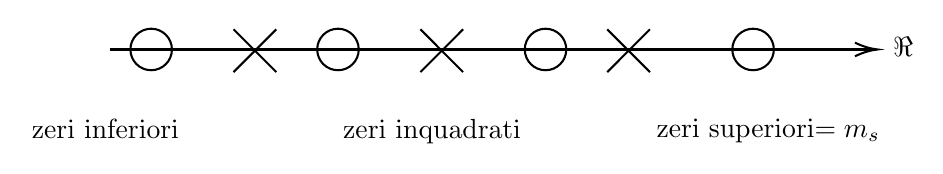
\begin{tikzpicture}[x=0.75pt,y=0.75pt,yscale=-1,xscale=1]
		%uncomment if require: \path (0,85); %set diagram left start at 0, and has height of 85
		
		\draw    (110,30) -- (478,30) ;
		\draw [shift={(480,30)}, rotate = 180] [color={rgb, 255:red, 0; green, 0; blue, 0 }  ][line width=0.75]    (10.93,-3.29) .. controls (6.95,-1.4) and (3.31,-0.3) .. (0,0) .. controls (3.31,0.3) and (6.95,1.4) .. (10.93,3.29)   ;
		\draw   (169.7,20.3) -- (190.3,40.91)(190.3,20.3) -- (169.7,40.91) ;
		\draw   (259.7,20.3) -- (280.3,40.91)(280.3,20.3) -- (259.7,40.91) ;
		\draw   (349.7,20.3) -- (370.3,40.91)(370.3,20.3) -- (349.7,40.91) ;
		%Shape: Circle [id:dp6909089299447624] 
		\draw   (120,30) .. controls (120,24.48) and (124.48,20) .. (130,20) .. controls (135.52,20) and (140,24.48) .. (140,30) .. controls (140,35.52) and (135.52,40) .. (130,40) .. controls (124.48,40) and (120,35.52) .. (120,30) -- cycle ;
		%Shape: Circle [id:dp2689895583644919] 
		\draw   (210,30) .. controls (210,24.48) and (214.48,20) .. (220,20) .. controls (225.52,20) and (230,24.48) .. (230,30) .. controls (230,35.52) and (225.52,40) .. (220,40) .. controls (214.48,40) and (210,35.52) .. (210,30) -- cycle ;
		%Shape: Circle [id:dp12206515426456699] 
		\draw   (410,30) .. controls (410,24.48) and (414.48,20) .. (420,20) .. controls (425.52,20) and (430,24.48) .. (430,30) .. controls (430,35.52) and (425.52,40) .. (420,40) .. controls (414.48,40) and (410,35.52) .. (410,30) -- cycle ;
		%Shape: Circle [id:dp2738635384059809] 
		\draw   (310,30) .. controls (310,24.48) and (314.48,20) .. (320,20) .. controls (325.52,20) and (330,24.48) .. (330,30) .. controls (330,35.52) and (325.52,40) .. (320,40) .. controls (314.48,40) and (310,35.52) .. (310,30) -- cycle ;
		
		\draw (486,22.4) node [anchor=north west][inner sep=0.75pt]    {$\Re$};
		\draw (71,62) node [anchor=north west][inner sep=0.75pt]   [align=left] {zeri inferiori};
		\draw (372,62) node [anchor=north west][inner sep=0.75pt]   [align=left] {zeri superiori$=m_s$};
		\draw (221,62) node [anchor=north west][inner sep=0.75pt]   [align=left] {zeri inquadrati};
		
		
	\end{tikzpicture}
	\\
	Uno zero è bene-inquadrato se tra i poli tra cui è compreso vede tanti zeri a destra quanti a sinistra\\
	
	
	
	
	\tikzset{every picture/.style={line width=0.75pt}} %set default line width to 0.75pt        
	
	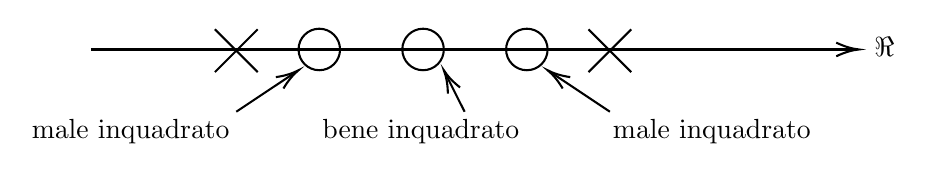
\begin{tikzpicture}[x=0.75pt,y=0.75pt,yscale=-1,xscale=1]
		%uncomment if require: \path (0,85); %set diagram left start at 0, and has height of 85
		
		\draw    (110,30) -- (478,30) ;
		\draw [shift={(480,30)}, rotate = 180] [color={rgb, 255:red, 0; green, 0; blue, 0 }  ][line width=0.75]    (10.93,-3.29) .. controls (6.95,-1.4) and (3.31,-0.3) .. (0,0) .. controls (3.31,0.3) and (6.95,1.4) .. (10.93,3.29)   ;
		\draw   (169.7,20.3) -- (190.3,40.91)(190.3,20.3) -- (169.7,40.91) ;
		\draw   (349.7,20.3) -- (370.3,40.91)(370.3,20.3) -- (349.7,40.91) ;
		%Shape: Circle [id:dp6235703732274369] 
		\draw   (210,30) .. controls (210,24.48) and (214.48,20) .. (220,20) .. controls (225.52,20) and (230,24.48) .. (230,30) .. controls (230,35.52) and (225.52,40) .. (220,40) .. controls (214.48,40) and (210,35.52) .. (210,30) -- cycle ;
		%Shape: Circle [id:dp011791331004185057] 
		\draw   (310,30) .. controls (310,24.48) and (314.48,20) .. (320,20) .. controls (325.52,20) and (330,24.48) .. (330,30) .. controls (330,35.52) and (325.52,40) .. (320,40) .. controls (314.48,40) and (310,35.52) .. (310,30) -- cycle ;
		%Shape: Circle [id:dp3877332279830781] 
		\draw   (260,30) .. controls (260,24.48) and (264.48,20) .. (270,20) .. controls (275.52,20) and (280,24.48) .. (280,30) .. controls (280,35.52) and (275.52,40) .. (270,40) .. controls (264.48,40) and (260,35.52) .. (260,30) -- cycle ;
		\draw    (180,60) -- (208.34,41.11) ;
		\draw [shift={(210,40)}, rotate = 506.31] [color={rgb, 255:red, 0; green, 0; blue, 0 }  ][line width=0.75]    (10.93,-3.29) .. controls (6.95,-1.4) and (3.31,-0.3) .. (0,0) .. controls (3.31,0.3) and (6.95,1.4) .. (10.93,3.29)   ;
		\draw    (360,60) -- (331.66,41.11) ;
		\draw [shift={(330,40)}, rotate = 393.69] [color={rgb, 255:red, 0; green, 0; blue, 0 }  ][line width=0.75]    (10.93,-3.29) .. controls (6.95,-1.4) and (3.31,-0.3) .. (0,0) .. controls (3.31,0.3) and (6.95,1.4) .. (10.93,3.29)   ;
		\draw    (290,60) -- (280.89,41.79) ;
		\draw [shift={(280,40)}, rotate = 423.43] [color={rgb, 255:red, 0; green, 0; blue, 0 }  ][line width=0.75]    (10.93,-3.29) .. controls (6.95,-1.4) and (3.31,-0.3) .. (0,0) .. controls (3.31,0.3) and (6.95,1.4) .. (10.93,3.29)   ;
		
		\draw (486,22.4) node [anchor=north west][inner sep=0.75pt]    {$\Re$};
		\draw (80,62) node [anchor=north west][inner sep=0.75pt]   [align=left] {male inquadrato};
		\draw (220,62) node [anchor=north west][inner sep=0.75pt]   [align=left] {bene inquadrato};
		\draw (360,62) node [anchor=north west][inner sep=0.75pt]   [align=left] {male inquadrato};
		
		
	\end{tikzpicture}
	\\
	Chiamiamo
	
	$\delta $ il numero degli zeri male inquadrati
	
	$m_s$ il numero degli zeri superiori
	
	$N$ il numero degli estremi.
	
	Allora
	\begin{equation*}
		\boxed{m_s \leq N\leq m_s +\delta }
	\end{equation*}
	Corollario:
	\begin{equation*}
		\boxed{
			\begin{array}{{>{\displaystyle}l}}
				m_s \ \text{dispari} \ \implies N\ \text{dispari} \\
				m_s \ \text{pari} \ \implies N\ \text{pari}       
			\end{array}
		}
	\end{equation*}
\end{thm}

Consideriamo un caso con lo \textit{zero instabile}.
\begin{equation*}
	G(s)=\frac{\mu (1+s\tau)}{(1+sT_1)(1+sT_2)}
\end{equation*}
con $T_1 ,T_2  >0$ per la stabilità, $\mu  >0$ a piacere, ma $\tau < 0$. Si ha quindi
\begin{equation*}
	y(0) =0\ \ \ \ \dot{y}(0) =\frac{\mu \tau }{T_1 T_2} < 0
\end{equation*}
parte verso il basso, con un estremo dato che $1\leq N\leq 1$.

Consideriamo un altro caso con zero nell'origine
\begin{equation*}
	G(s)=\frac{\mu s}{(1+sT_1)(1+sT_2)}
\end{equation*}
con $T_1 ,T_2  >0$ per la stabilità, $\mu  >0$ a piacere. Si ha quindi
\begin{equation*}
	y(0) =0\ \ \ \ \dot{y}(0) =\frac{\mu }{T_1 T_2}  >0
\end{equation*}
Notiamo che è un sistema a guadagno nullo $G(0) =0$
\begin{equation*}
	\overline{y} =G(0)\overline{u} =0
\end{equation*}
Qui $\mu $ non coincide col guadagno.

Cosa succede quando la $G(s)$ ha poli complessi? Introduciamo una forma standard da usare quando ha due poli complessi. Con $\alpha _1 ,\alpha _2  >0$ per la stabilità
\begin{equation*}
	G(s) =\frac{\beta _2}{s^2 +\alpha _1 s+\alpha _2} =\mu \frac{\omega ^2_n}{s^2 +2\xi \omega _n s+\omega ^2_n}
\end{equation*}
Con $\omega _n  >0$ \textbf{pulsazione naturale} e $\xi $ \textbf{smorzamento}.

La presenza di $\mu $ e $\omega ^2_n$ a numeratore permette di lasciare a $\mu $ il ruolo di guadagno:
\begin{equation*}
	G(0) =\mu \frac{\omega ^2_n}{\omega ^2_n} =\mu 
\end{equation*}
I poli valgono
\begin{equation*}
	\begin{aligned}
		p_{1,2} & =-\xi \omega _n \pm \sqrt{\xi ^2 \omega ^2_n -\omega ^2_n} \\
		        & =-\xi \omega _n \pm \omega _n\sqrt{\xi ^2 -1}              
	\end{aligned}
\end{equation*}
L'ipotesi affinché siano \textit{complessi} e che ci sia \textit{stabilità} è $0< \xi < 1$
\begin{equation*}
	p_{1,2} =-\xi \omega _n \pm i\omega _n\sqrt{1-\xi ^2} \ \ \implies \ \ T=-\frac{1}{\Re(p)} =\frac{1}{\xi \omega _n}
\end{equation*}
Qui $r=2$, allora
\begin{gather*}
	y(0) =0\\
	\dot{y}(0) =0\\
	\ddot{y}(0) =\mu \omega ^2_n  >0
\end{gather*}
Si hanno oscillazioni, la distanza tra gli estremi (che sono infiniti) rimane costante e vale
\begin{equation*}
	\boxed{\tau =\frac{2\pi }{\Im(p)}}
\end{equation*}
ci sfugge anche qui l'ampiezza della sovraelongazione, che si quantifica con
\begin{equation*}
	\boxed{S=\frac{y_{\text{max}} -y(\infty)}{y(\infty)}}
\end{equation*}

Cosa significa invece avere una $G(s)$ fatta come
\begin{equation*}
	G(s) =\tilde{G}(s) e^{-sT} ,\ \ T >0
\end{equation*}
con $\tilde{G}(s)$ razionale fratta? Ricordiamo il risultato della traslazione (7). Possiamo pensare il sistema come una cascata

\begin{figure}[htpb]\centering
	\tikzset{every picture/.style={line width=0.75pt}} %set default line width to 0.75pt        
	
	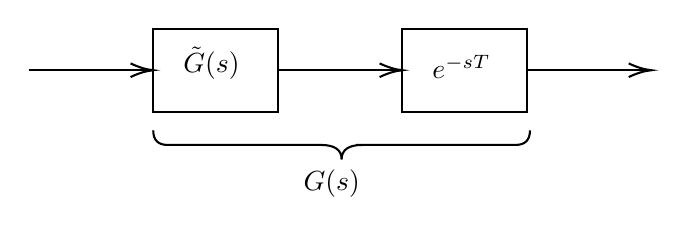
\begin{tikzpicture}[x=0.75pt,y=0.75pt,yscale=-1,xscale=1]
		%uncomment if require: \path (0,102); %set diagram left start at 0, and has height of 102
		
		%Shape: Rectangle [id:dp17826137817386312] 
		\draw   (160,10) -- (220,10) -- (220,50) -- (160,50) -- cycle ;
		\draw    (220,30) -- (278,30) ;
		\draw [shift={(280,30)}, rotate = 180] [color={rgb, 255:red, 0; green, 0; blue, 0 }  ][line width=0.75]    (10.93,-3.29) .. controls (6.95,-1.4) and (3.31,-0.3) .. (0,0) .. controls (3.31,0.3) and (6.95,1.4) .. (10.93,3.29)   ;
		\draw    (100,30) -- (158,30) ;
		\draw [shift={(160,30)}, rotate = 180] [color={rgb, 255:red, 0; green, 0; blue, 0 }  ][line width=0.75]    (10.93,-3.29) .. controls (6.95,-1.4) and (3.31,-0.3) .. (0,0) .. controls (3.31,0.3) and (6.95,1.4) .. (10.93,3.29)   ;
		%Shape: Rectangle [id:dp9049460323970084] 
		\draw   (280,10) -- (340,10) -- (340,50) -- (280,50) -- cycle ;
		\draw    (340,30) -- (398,30) ;
		\draw [shift={(400,30)}, rotate = 180] [color={rgb, 255:red, 0; green, 0; blue, 0 }  ][line width=0.75]    (10.93,-3.29) .. controls (6.95,-1.4) and (3.31,-0.3) .. (0,0) .. controls (3.31,0.3) and (6.95,1.4) .. (10.93,3.29)   ;
		%Shape: Brace [id:dp6018538731060217] 
		\draw   (160,59) .. controls (160,63.67) and (162.33,66) .. (167,66) -- (240.75,66) .. controls (247.42,66) and (250.75,68.33) .. (250.75,73) .. controls (250.75,68.33) and (254.08,66) .. (260.75,66)(257.75,66) -- (334.5,66) .. controls (339.17,66) and (341.5,63.67) .. (341.5,59) ;
		
		\draw (173,17.4) node [anchor=north west][inner sep=0.75pt]    {$\tilde{G}(s)$};
		\draw (293,21.4) node [anchor=north west][inner sep=0.75pt]    {$e^{-sT}$};
		\draw (231,76.4) node [anchor=north west][inner sep=0.75pt]    {$G(s)$};
		
		
	\end{tikzpicture}
\end{figure}\FloatBarrier

Vediamo quindi che il termine $e^{-sT}$ induce un ritardo di $T$, si chiama \textbf{ritardatore puro}.

\chapter{Regime sinusoidale}

Consideriamo ingressi del tipo
\begin{equation*}
	u_T(t) =U\sin\left(\frac{2\pi }{T} t\right)
\end{equation*}
Si introducono altre grandezze
\begin{equation*}
	\omega =\frac{2\pi }{T} =2\pi f\ \ \ \ f=\frac{1}{T}
\end{equation*}
allora
\begin{equation*}
	u_T(t) =U\sin(\omega t) =U\sin(2\pi f\cdotp t)
\end{equation*}
Studiare il regime sinusoidale significa studiare tutti i regimi periodici che possono essere scritti come somma di sinusoidi per Fourier:
\begin{equation*}
	u(t) =U_0 +\sum\limits ^{\infty }_{k=1} U_k\sin\left(k\frac{2\pi }{T} t+\varphi _k\right) ,\ \ k\in \mathbb{N}
\end{equation*}
Affinché ci sia convergenza della serie è necessario, ma non sufficiente, che $U_k\xrightarrow{k\to \infty } 0$.
\begin{thm}
	Sia $G(s) =\frac{N(s)}{\Delta (s)}$, immaginiamo che sia compl. oss. e compl. ragg., quindi il modello esterno descrive completamente il sistema, altrimenti potremmo fare poco. Supponiamo che risponda all'ingresso $u_T(t) =U\sin(\omega t) ,\omega =2\pi /T$. Allora $\exists !$ uscita sinusoidale
	\begin{equation*}
		y_T(t) =Y\sin(\omega t+\varphi) \ \ \iff \ \ \Delta (i\omega) \neq 0
	\end{equation*}
	In tal caso
	\begin{equation*}
		\frac{Y}{U} =R(\omega) ,\ \ \varphi =\varphi (\omega)
	\end{equation*}
	$R(\omega) ,\varphi (\omega)$ sono dette \textbf{risposta in frequenza}.
\end{thm}
La condizione $\Delta (i\omega) \neq 0$ chiede che \textbf{non ci siano autovalori di modulo} $\omega $.

Possiamo scrivere $G(s) =\frac{N(s)}{\Delta (s)}$ come
\begin{equation*}
	\Delta (s) y=N(s) u\ \ \iff \ \ y^{(n)}(t) +\cdots +\alpha _n y(t) =\beta _0 u^{(n)}(t) +\cdots +\beta _n u(t)
\end{equation*}
e ognuna di queste equazioni differenziali, per ogni set di condizioni iniziali diverse, produrrà diverse uscite, che possiamo genericamente chiamare $y$, mentre una sola di queste sarà quella sinusoidale $y_T$. Scriviamole
\begin{gather*}
	\Delta (s) y_T =N(s) u_T\\
	\Delta (s) y=N(s) u_T
\end{gather*}
Sottraiamo membro a membro
\begin{equation*}
	\begin{aligned}
		\Delta (s)(y-y_T) & =0 \\
		\Delta (s) e      & =0 
	\end{aligned}
\end{equation*}
Ma se il sistema è asint. stabile
\begin{equation*}
	e(t)\to 0\ \forall e(0) \ \ \iff \ \ y(t)\to y_T(t)
\end{equation*}
Quindi per ogni condizione iniziale tendiamo alla sinusoide.

\begin{figure}[htpb]\centering
	\tikzset{every picture/.style={line width=0.75pt}} %set default line width to 0.75pt        
	
	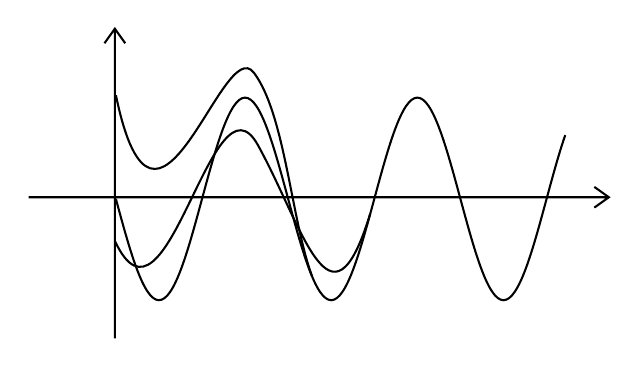
\begin{tikzpicture}[x=0.75pt,y=0.75pt,yscale=-1,xscale=1]
		%uncomment if require: \path (0,171); %set diagram left start at 0, and has height of 171
		
		%Shape: Axis 2D [id:dp7058071342841148] 
		\draw  (118,91.2) -- (397.5,91.2)(159.5,10) -- (159.5,159.2) (390.5,86.2) -- (397.5,91.2) -- (390.5,96.2) (154.5,17) -- (159.5,10) -- (164.5,17)  ;
		%Shape: Wave [id:dp1383928221499804] 
		\draw   (160,92) .. controls (166.77,117) and (173.24,140.8) .. (180.75,140.8) .. controls (188.26,140.8) and (194.73,117) .. (201.5,92) .. controls (208.27,67) and (214.74,43.2) .. (222.25,43.2) .. controls (229.76,43.2) and (236.23,67) .. (243,92) .. controls (249.77,117) and (256.24,140.8) .. (263.75,140.8) .. controls (271.26,140.8) and (277.73,117) .. (284.5,92) .. controls (291.27,67) and (297.74,43.2) .. (305.25,43.2) .. controls (312.76,43.2) and (319.23,67) .. (326,92) .. controls (332.77,117) and (339.24,140.8) .. (346.75,140.8) .. controls (354.26,140.8) and (360.73,117) .. (367.5,92) .. controls (370.52,80.85) and (373.48,69.93) .. (376.5,61.26) ;
		%Curve Lines [id:da46544665128863305] 
		\draw    (160,42) .. controls (179.5,136.2) and (211.5,11.2) .. (226.5,31.2) .. controls (241.5,51.2) and (244.5,102.2) .. (254.5,129.2) ;
		%Curve Lines [id:da8157023906435408] 
		\draw    (159.5,112.2) .. controls (184.5,166.2) and (206.5,26.2) .. (228.5,66.2) .. controls (250.5,106.2) and (263.5,161.2) .. (282.5,99.2) ;
		
		
		
		
	\end{tikzpicture}
\end{figure}\FloatBarrier

\begin{thm}
	Se $\Delta (i\omega) \neq 0$ e $u_T(t) =U\sin(\omega t)$ sappiamo che $y_T(t) =Y\sin(\omega t+\varphi)$. Allora
	\begin{equation*}
		\boxed{
			\frac{Y}{U} =| G(i\omega)| \ \ \ \ \varphi =\arg G(i\omega) ,\ \varphi \in [ -\pi ,\pi)
		}
	\end{equation*}
\end{thm}

\section{Risposta in frequenza}

Studiamo per ora
\begin{equation*}
	G(s) =\frac{\mu }{1+sT} ,\quad\mu,T  >0
\end{equation*}
Allora
\begin{equation*}
	G(i\omega) =\frac{\mu }{1+i\omega T } \ \ \implies \ \ \frac{Y}{U} =| G(i\omega)| =\frac{\mu }{\sqrt{1+\omega ^2T^2}} ,\ \ \varphi =\arg G(i\omega) =-\arctan (\omega T) 
\end{equation*}

\begin{figure}[htpb]\centering    
% esempio: mu = 3, T = 1
\begin{minipage}{0.48\textwidth}
    \centering
	\begin{tikzpicture}[domain=0:7]
    \draw[->] (-0.5,0) -- (7.2,0) node[below right] {$\omega$};
    \draw[->] (0,-0.2) -- (0,4) node[left] {$|G(i\omega)|$};
    \node[below left] at (0,0) {$0$};
    \draw[smooth] plot (\x,{3/sqrt(1+\x^2)});
    \node[left] at (0,3) {$\mu = G_\text{max}$};
    \draw[dashed] (0,{3/sqrt(2)}) node[left] {$\frac{G_\text{max}}{\sqrt{2}}$} -- (1,{3/sqrt(2)});
    \draw[dashed] (1,0) node[below] {$\bar \omega$} -- (1,{3/sqrt(2)});
	\end{tikzpicture}
\end{minipage}
\hspace{0.025\textwidth}
\begin{minipage}{0.48\textwidth}
    \centering
    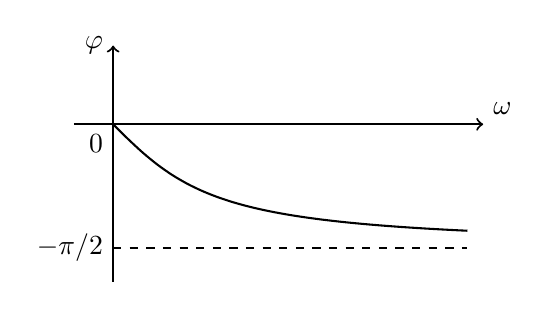
\begin{tikzpicture}[domain=0:4.5]
        \draw[->] (-0.5,0) -- (4.7,0) node[above right] {$\omega$};
        \draw[->] (0,-2) -- (0,1) node[left] {$\varphi$};
        \node[below left] at (0,0) {$0$};
        \draw[smooth] plot (\x,{-atan(\x)*pi/180});
        \draw[dashed] (0,{-pi/2}) node[left] {$-\pi/2$} -- (4.5,{-pi/2});
    \end{tikzpicture}
\end{minipage}
\end{figure}\FloatBarrier

Il sistema si dice \textbf{filtro passa basso}, $\bar \omega $ è la \textbf{frequenza di taglio}. Definiamo inoltre
\begin{equation*}
	BP\ =\ \text{Banda passante} \ :=\left\{\omega :\ \frac{G_{\text{max}}}{\sqrt{2}} \leq | G(i\omega)| \leq G_{\text{max}}\right\}
\end{equation*}

Se studiamo
\begin{equation*}
	G(s) =\frac{\mu s}{1+s} ,\ \mu  >0
\end{equation*}
Allora
\begin{equation*}
	G(i\omega) =\frac{\mu i\omega }{1+i\omega } \ \ \implies \ \ | G(i\omega)| =\frac{\mu \omega }{\sqrt{1+\omega ^2}} ,\ \ \arg G(i\omega) =\frac{\pi }{2} -\arctan \omega 
\end{equation*}

\begin{figure}[htpb]\centering    
% esempio: mu = 3
\begin{minipage}{0.48\textwidth}
    \centering
	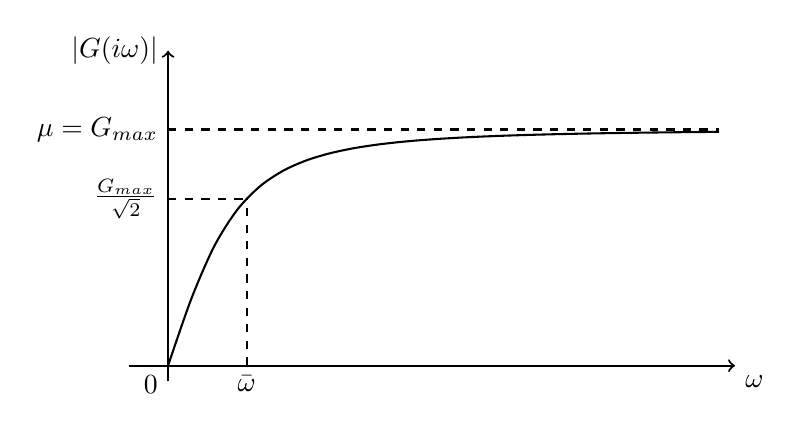
\begin{tikzpicture}[domain=0:7]
    \draw[->] (-0.5,0) -- (7.2,0) node[below right] {$\omega$};
    \draw[->] (0,-0.2) -- (0,4) node[left] {$|G(i\omega)|$};
    \node[below left] at (0,0) {$0$};
    \draw[smooth] plot (\x,{3*\x /sqrt(1+\x^2)});
    \draw[dashed] (0,3) node[left] {$\mu = G_\text{max}$} -- (7,3);
    \draw[dashed] (0,{3/sqrt(2)}) node[left] {$\frac{G_\text{max}}{\sqrt{2}}$} -- (1,{3/sqrt(2)});
    \draw[dashed] (1,0) node[below] {$\bar \omega$} -- (1,{3/sqrt(2)});
    
	\end{tikzpicture}
\end{minipage}
\hspace{0.025\textwidth}
\begin{minipage}{0.48\textwidth}
    \centering
    \begin{tikzpicture}[domain=0:4.5]
        \draw[->] (-0.5,0) -- (4.7,0) node[above right] {$\omega$};
        \draw[->] (0,-0.2) -- (0,2.5) node[left] {$\varphi$};
        \node[below left] at (0,0) {$0$};
        \draw[smooth] plot (\x,{pi/2-atan(\x)*pi/180});
        \node[left] at (0,{pi/2}) {$\pi/2$};
    \end{tikzpicture}
\end{minipage}
\end{figure}\FloatBarrier

È un \textbf{filtro passa alto}.

Se studiamo
\begin{equation*}
	G(s) =\frac{\mu s}{(1+s)(1+0.1s)} ,\ \mu  >0
\end{equation*}
Allora
\begin{gather*}
	G(i\omega) =\frac{\mu i\omega }{(1+i\omega)(1+0.1i\omega)}\\
	\Downarrow \\
	| G(i\omega)| =\frac{\mu \omega }{\sqrt{1+\omega ^2}\sqrt{1+0.01\omega ^2}} ,\ \ \arg G(i\omega) =\frac{\pi }{2} -\arctan \omega -\arctan(0.1\omega)
\end{gather*}

\begin{figure}[htpb]\centering    
% esempio: mu = 3, in scala per rappresentare anche l'andamento a omega alti
\begin{minipage}{0.48\textwidth}
    \centering
	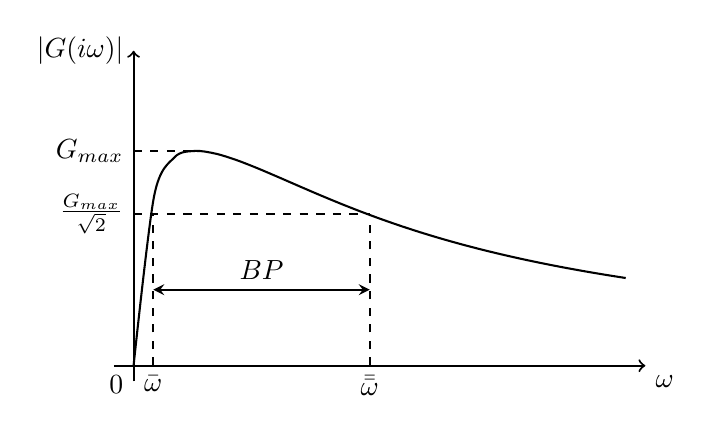
\begin{tikzpicture}[domain=0:25, xscale=0.25]
    \draw[->] (-1,0) -- (26,0) node[below right] {$\omega$};
    \draw[->] (0,-0.2) -- (0,4) node[left] {$|G(i\omega)|$};
    \node[below left] at (0,0) {$0$};
    \draw[smooth] plot (\x,{3*\x /sqrt((1+\x^2)*(1+0.01*\x^2))});
    \draw[dashed] (0,2.73) node[left] {$G_\text{max}$} -- (3.5,2.73);
    \draw[dashed] (0,{2.73/sqrt(2)}) node[left] {$\frac{G_\text{max}}{\sqrt{2}}$} -- (12,{2.73/sqrt(2)});
    \draw[dashed] (1,0) node[below] {$\bar \omega$} -- (1,{2.73/sqrt(2)});
    \draw[dashed] (12,0) node[below] {$\bar {\bar \omega}$} -- (12,{2.73/sqrt(2)});
    \draw[<->, >=stealth] (1,{2.73/(2*sqrt(2))}) -- (12,{2.73/(2*sqrt(2))}) node[midway, above] {$BP$};
    
	\end{tikzpicture}
\end{minipage}
\hspace{0.025\textwidth}
\begin{minipage}{0.48\textwidth}
    \centering
    \begin{tikzpicture}[domain=0:20,xscale=0.25]
        \draw[->] (-1,0) -- (20,0) node[above right] {$\omega$};
        \draw[->] (0,-2) -- (0,2.2) node[left] {$\varphi$};
        \node[below left] at (0,0) {$0$};
        \draw[smooth] plot (\x,{pi/2-atan(\x)*pi/180-atan(0.1*\x)*pi/180});
        \node[left] at (0,{pi/2}) {$\pi/2$};
        \draw[dashed] (0,{-pi/2}) node[left] {$-\pi/2$} -- (20,{-pi/2});
    \end{tikzpicture}
\end{minipage}
\caption{Modulo e fase di $G(i\omega)$ in funzione di $\omega$. L'asse delle ascisse è in scala 1:4.}
\end{figure}\FloatBarrier

È un \textbf{filtro passa banda}.

\section{Diagrammi di Bode}

Ipotizziamo di avere poli e zeri tutti reali, introduciamo una forma standard di $G(s)$
\begin{equation*}
	\boxed{G(s) =\frac{\mu }{s^h} \cdot \frac{\prod _j(1+s\tau _j)}{\prod _j(1+sT_j)}}
\end{equation*}
I poli e zeri saranno della forma
\begin{equation*}
	z_j =-\frac{1}{\tau _j} \ \ \ \ p_j =-\frac{1}{T_j}
\end{equation*}
Il valore $h$ si dice \textbf{tipo} del sistema, è intero. Se $h=1$ c'è un \textbf{polo dell'origine}, se $h=2,3,\dotsc $ ci sono poli multipli in $0$. Se $h=-1$ c'è uno \textbf{zero nell'origine}. $\mu $ si dice \textbf{guadagno generalizzato}, è parente del guadagno che avevamo introdotto, ma non sempre lo stesso proprio perché c'è quel $s^h$ che dà problemi ogni volta che $h\neq 0$.

Introduciamo un asse logaritmico in base $10$
\begin{equation*}
	v=\log_{10} \omega \ \ \iff \ \ \omega =10^v
\end{equation*}

\begin{figure}[htpb]\centering
	\tikzset{every picture/.style={line width=0.75pt}} %set default line width to 0.75pt        
	
	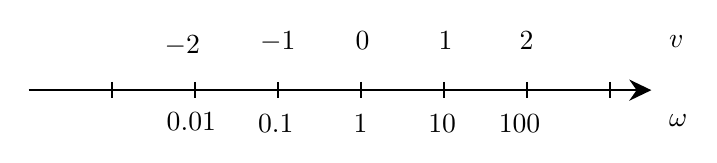
\begin{tikzpicture}[x=0.75pt,y=0.75pt,yscale=-1,xscale=1]
		%uncomment if require: \path (0,67); %set diagram left start at 0, and has height of 67
		
		\draw    (100,30) -- (397,30) (140,26) -- (140,34)(180,26) -- (180,34)(220,26) -- (220,34)(260,26) -- (260,34)(300,26) -- (300,34)(340,26) -- (340,34)(380,26) -- (380,34) ;
		\draw [shift={(400,30)}, rotate = 180] [fill={rgb, 255:red, 0; green, 0; blue, 0 }  ][line width=0.08]  [draw opacity=0] (10.72,-5.15) -- (0,0) -- (10.72,5.15) -- (7.12,0) -- cycle    ;
		
		\draw (407,2.4) node [anchor=north west][inner sep=0.75pt]    {$v$};
		\draw (407,40.4) node [anchor=north west][inner sep=0.75pt]    {$\omega $};
		\draw (164,2.4) node [anchor=north west][inner sep=0.75pt]    {$-2$};
		\draw (210,0.4) node [anchor=north west][inner sep=0.75pt]    {$-1$};
		\draw (256,0.4) node [anchor=north west][inner sep=0.75pt]    {$0$};
		\draw (296,0.4) node [anchor=north west][inner sep=0.75pt]    {$1$};
		\draw (335,0.4) node [anchor=north west][inner sep=0.75pt]    {$2$};
		\draw (165,39.4) node [anchor=north west][inner sep=0.75pt]    {$0.01$};
		\draw (209,40.4) node [anchor=north west][inner sep=0.75pt]    {$0.1$};
		\draw (255,40.4) node [anchor=north west][inner sep=0.75pt]    {$1$};
		\draw (291,40.4) node [anchor=north west][inner sep=0.75pt]    {$10$};
		\draw (325,40.4) node [anchor=north west][inner sep=0.75pt]    {$100$};
		
		
	\end{tikzpicture}
\end{figure}\FloatBarrier

Si noti che non troviamo mai $\omega =0$. L'intervallo tra due tacchette del grafico si chiama \textbf{decade}.

\subsection{Diagrammi di Bode del modulo}

Sull'asse delle ordinate rappresenteremo il modulo di $G(i\omega)$ in decibel
\begin{equation*}
	\boxed{| G(i\omega)| _{\si{dB}} =20\log_{10}| G(i\omega)| }
\end{equation*}

\begin{figure}[htpb]\centering
	\tikzset{every picture/.style={line width=0.75pt}} %set default line width to 0.75pt        
	
	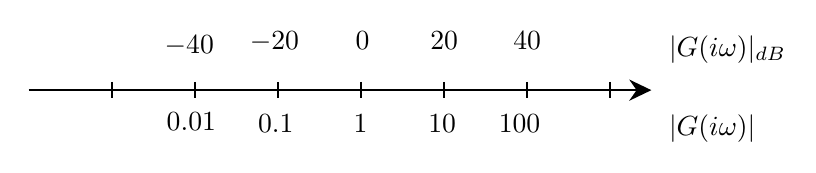
\begin{tikzpicture}[x=0.75pt,y=0.75pt,yscale=-1,xscale=1]
		%uncomment if require: \path (0,67); %set diagram left start at 0, and has height of 67
		
		\draw    (100,30) -- (397,30) (140,26) -- (140,34)(180,26) -- (180,34)(220,26) -- (220,34)(260,26) -- (260,34)(300,26) -- (300,34)(340,26) -- (340,34)(380,26) -- (380,34) ;
		\draw [shift={(400,30)}, rotate = 180] [fill={rgb, 255:red, 0; green, 0; blue, 0 }  ][line width=0.08]  [draw opacity=0] (10.72,-5.15) -- (0,0) -- (10.72,5.15) -- (7.12,0) -- cycle    ;
		
		\draw (407,2.4) node [anchor=north west][inner sep=0.75pt]    {$| G(i\omega)| _{\si{dB}}$};
		\draw (407,40.4) node [anchor=north west][inner sep=0.75pt]    {$| G(i\omega)| $};
		\draw (164,2.4) node [anchor=north west][inner sep=0.75pt]    {$-40$};
		\draw (205,0.4) node [anchor=north west][inner sep=0.75pt]    {$-20$};
		\draw (256,0.4) node [anchor=north west][inner sep=0.75pt]    {$0$};
		\draw (292,0.4) node [anchor=north west][inner sep=0.75pt]    {$20$};
		\draw (332,0.4) node [anchor=north west][inner sep=0.75pt]    {$40$};
		\draw (165,39.4) node [anchor=north west][inner sep=0.75pt]    {$0.01$};
		\draw (209,40.4) node [anchor=north west][inner sep=0.75pt]    {$0.1$};
		\draw (255,40.4) node [anchor=north west][inner sep=0.75pt]    {$1$};
		\draw (291,40.4) node [anchor=north west][inner sep=0.75pt]    {$10$};
		\draw (325,40.4) node [anchor=north west][inner sep=0.75pt]    {$100$};
		
		
	\end{tikzpicture}
\end{figure}\FloatBarrier

Consideriamo
\begin{equation*}
	| G(i\omega)| =\frac{| \mu | }{\omega ^h} \cdot \frac{\prod _j| 1+i\omega \tau _j| }{\prod _j| 1+i\omega T_j| }
\end{equation*}
Il logaritmo trasforma prodotti e divisioni in somme e sottrazioni
\begin{equation*}
	\boxed{| G(i\omega)| _{\si{dB}} =20\log| \mu | -20h\log \omega +{\textstyle \sum\nolimits _j 20\log| 1+i\omega \tau _j| -\sum\nolimits _j 20\log| 1+i\omega T_j| }}
\end{equation*}
Se riusciamo a rappresentarle individualmente sarà la somma di ciascuna di queste, è un'ottima notizia.
\begin{itemize}
	\item pezzo $20\log| \mu | $, è costante
	      
	      \begin{figure}[htpb]\centering
	      	\tikzset{every picture/.style={line width=0.75pt}} %set default line width to 0.75pt        
	      	
	      	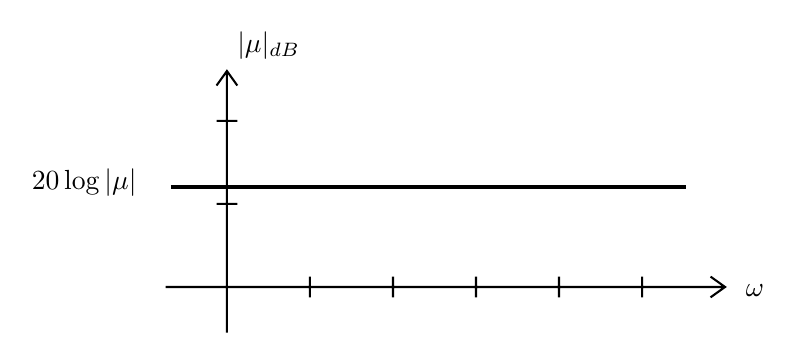
\begin{tikzpicture}[x=0.75pt,y=0.75pt,yscale=-1,xscale=1]
	      		%uncomment if require: \path (0,169); %set diagram left start at 0, and has height of 169
	      		
	      		%Shape: Axis 2D [id:dp9422657456008035] 
	      		\draw  (90,136.83) -- (359.5,136.83)(119.5,32.78) -- (119.5,158.78) (352.5,131.83) -- (359.5,136.83) -- (352.5,141.83) (114.5,39.78) -- (119.5,32.78) -- (124.5,39.78) (159.5,131.83) -- (159.5,141.83)(199.5,131.83) -- (199.5,141.83)(239.5,131.83) -- (239.5,141.83)(279.5,131.83) -- (279.5,141.83)(319.5,131.83) -- (319.5,141.83)(114.5,96.83) -- (124.5,96.83)(114.5,56.83) -- (124.5,56.83) ;
	      		\draw   ;
	      		\draw [line width=1.5]    (92.5,88.78) -- (340.5,88.78) ;
	      		
	      		\draw (368,134.4) node [anchor=north west][inner sep=0.75pt]    {$\omega $};
	      		\draw (123,12.4) node [anchor=north west][inner sep=0.75pt]    {$| \mu | _{\si{dB}}$};
	      		\draw (24,78.4) node [anchor=north west][inner sep=0.75pt]    {$20\log| \mu | $};
	      		
	      		
	      	\end{tikzpicture}
	      \end{figure}\FloatBarrier
	      
	\item pezzo $-20h\log \omega =-20hv$, su un'asse che in $v$ è lineare! È una retta con pendenza $-20h$. Se $h=1$, ogni unità in $v$, cala di $20$ e passa per $0$ quando $v=0$, cioè quando $\omega =1$. Si dice che la pendenza è $20\si{dB/dec}$
	      
	      \begin{figure}[htpb]\centering
	      	\tikzset{every picture/.style={line width=0.75pt}} %set default line width to 0.75pt        
	      	
	      	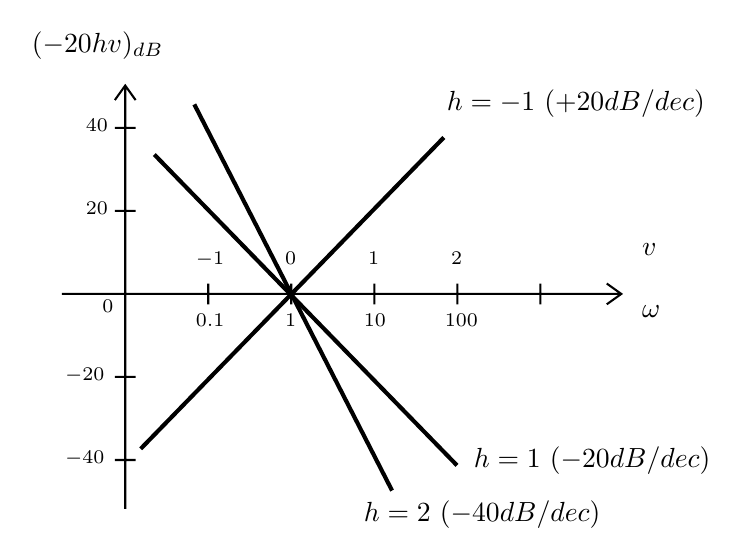
\begin{tikzpicture}[x=0.75pt,y=0.75pt,yscale=-1,xscale=1]
	      		%uncomment if require: \path (0,267); %set diagram left start at 0, and has height of 267
	      		
	      		%Shape: Axis 2D [id:dp3673165074083895] 
	      		\draw  (70,146.18) -- (339.5,146.18)(100.5,45.78) -- (100.5,249.78) (332.5,141.18) -- (339.5,146.18) -- (332.5,151.18) (95.5,52.78) -- (100.5,45.78) -- (105.5,52.78) (140.5,141.18) -- (140.5,151.18)(180.5,141.18) -- (180.5,151.18)(220.5,141.18) -- (220.5,151.18)(260.5,141.18) -- (260.5,151.18)(300.5,141.18) -- (300.5,151.18)(95.5,106.18) -- (105.5,106.18)(95.5,66.18) -- (105.5,66.18)(95.5,186.18) -- (105.5,186.18)(95.5,226.18) -- (105.5,226.18) ;
	      		\draw   ;
	      		\draw [line width=1.5]    (114.5,79) -- (260.34,228.78) ;
	      		%Shape: Boxed Line [id:dp758692919096021] 
	      		\draw [line width=1.5]    (254.03,70.78) -- (107.97,220.78) ;
	      		\draw [line width=1.5]    (133.78,54.85) -- (229.06,240.93) ;
	      		
	      		\draw (348,150.4) node [anchor=north west][inner sep=0.75pt]    {$\omega $};
	      		\draw (54,18.4) node [anchor=north west][inner sep=0.75pt]    {$(-20hv)_{\si{dB}}$};
	      		\draw (176,154.4) node [anchor=north west][inner sep=0.75pt]  [font=\scriptsize]  {$1$};
	      		\draw (176,124.4) node [anchor=north west][inner sep=0.75pt]  [font=\scriptsize]  {$0$};
	      		\draw (214,154.4) node [anchor=north west][inner sep=0.75pt]  [font=\scriptsize]  {$10$};
	      		\draw (216,124.4) node [anchor=north west][inner sep=0.75pt]  [font=\scriptsize]  {$1$};
	      		\draw (253,154.4) node [anchor=north west][inner sep=0.75pt]  [font=\scriptsize]  {$100$};
	      		\draw (256,124.4) node [anchor=north west][inner sep=0.75pt]  [font=\scriptsize]  {$2$};
	      		\draw (348,120.4) node [anchor=north west][inner sep=0.75pt]    {$v$};
	      		\draw (133,124.4) node [anchor=north west][inner sep=0.75pt]  [font=\scriptsize]  {$-1$};
	      		\draw (133,154.4) node [anchor=north west][inner sep=0.75pt]  [font=\scriptsize]  {$0.1$};
	      		\draw (88,147.4) node [anchor=north west][inner sep=0.75pt]  [font=\scriptsize]  {$0$};
	      		\draw (80,100.4) node [anchor=north west][inner sep=0.75pt]  [font=\scriptsize]  {$20$};
	      		\draw (80,60.4) node [anchor=north west][inner sep=0.75pt]  [font=\scriptsize]  {$40$};
	      		\draw (70,180.4) node [anchor=north west][inner sep=0.75pt]  [font=\scriptsize]  {$-20$};
	      		\draw (70,220.4) node [anchor=north west][inner sep=0.75pt]  [font=\scriptsize]  {$-40$};
	      		\draw (254,46.18) node [anchor=north west][inner sep=0.75pt]    {$h=-1\ (+20\si{dB/dec})$};
	      		\draw (267,218.18) node [anchor=north west][inner sep=0.75pt]    {$h=1\ (-20\si{dB/dec})$};
	      		\draw (214,244.18) node [anchor=north west][inner sep=0.75pt]    {$h=2\ (-40\si{dB/dec})$};
	      		
	      		
	      	\end{tikzpicture}
	      \end{figure}\FloatBarrier
	      
	      
	      Sommando i primi due pezzi si vede che a $\omega =1$, il modulo vale $\mu $ espresso in decibel.
	\item pezzo ${\textstyle f=20\log| 1+i\omega \tau | =20\log\sqrt{1+\omega ^2 \tau ^2}}$
	      
	      se $\omega \to 0$ allora $f \to 0$
	      
	      se $\omega \to +\infty$ allora $f\to 20\log(\omega | \tau |) =20\log \omega +20\log| \tau | $, questa quantità è $0$ per $\omega =\frac{1}{| \tau | }$
	      
	      \begin{figure}[htpb]\centering
	      	\tikzset{every picture/.style={line width=0.75pt}} %set default line width to 0.75pt        
	      	
	      	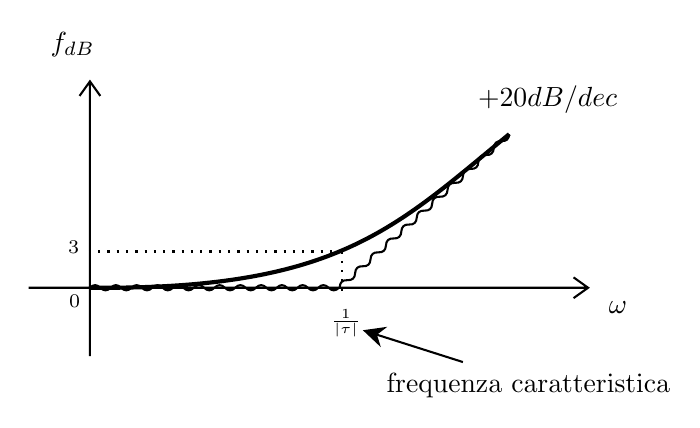
\begin{tikzpicture}[x=0.75pt,y=0.75pt,yscale=-1,xscale=1]
	      		%uncomment if require: \path (0,205); %set diagram left start at 0, and has height of 205
	      		
	      		%Shape: Axis 2D [id:dp18900085337753092] 
	      		\draw  (50,135.2) -- (319.5,135.2)(79.5,35.78) -- (79.5,168.2) (312.5,130.2) -- (319.5,135.2) -- (312.5,140.2) (74.5,42.78) -- (79.5,35.78) -- (84.5,42.78)  ;
	      		\draw    (281.5,61.2) .. controls (281.38,63.55) and (280.14,64.67) .. (277.79,64.55) .. controls (275.44,64.43) and (274.2,65.55) .. (274.08,67.9) .. controls (273.95,70.25) and (272.71,71.37) .. (270.36,71.25) .. controls (268.01,71.13) and (266.77,72.25) .. (266.65,74.6) .. controls (266.53,76.95) and (265.29,78.07) .. (262.94,77.95) .. controls (260.59,77.83) and (259.35,78.95) .. (259.23,81.3) .. controls (259.11,83.65) and (257.87,84.77) .. (255.52,84.65) .. controls (253.17,84.53) and (251.93,85.65) .. (251.8,88) .. controls (251.68,90.35) and (250.44,91.47) .. (248.09,91.35) .. controls (245.74,91.23) and (244.5,92.35) .. (244.38,94.7) .. controls (244.26,97.05) and (243.02,98.17) .. (240.67,98.05) .. controls (238.32,97.93) and (237.08,99.05) .. (236.96,101.4) .. controls (236.83,103.75) and (235.59,104.87) .. (233.24,104.75) .. controls (230.89,104.63) and (229.65,105.75) .. (229.53,108.1) .. controls (229.41,110.45) and (228.17,111.57) .. (225.82,111.45) .. controls (223.47,111.33) and (222.23,112.45) .. (222.11,114.8) .. controls (221.99,117.15) and (220.75,118.27) .. (218.4,118.15) .. controls (216.05,118.03) and (214.81,119.15) .. (214.68,121.5) .. controls (214.56,123.85) and (213.32,124.97) .. (210.97,124.85) .. controls (208.62,124.73) and (207.38,125.85) .. (207.26,128.2) .. controls (207.14,130.55) and (205.9,131.67) .. (203.55,131.55) .. controls (201.2,131.43) and (199.96,132.55) .. (199.84,134.9) -- (199.5,135.2) -- (199.5,135.2) .. controls (197.83,136.87) and (196.17,136.87) .. (194.5,135.2) .. controls (192.83,133.53) and (191.17,133.53) .. (189.5,135.2) .. controls (187.83,136.87) and (186.17,136.87) .. (184.5,135.2) .. controls (182.83,133.53) and (181.17,133.53) .. (179.5,135.2) .. controls (177.83,136.87) and (176.17,136.87) .. (174.5,135.2) .. controls (172.83,133.53) and (171.17,133.53) .. (169.5,135.2) .. controls (167.83,136.87) and (166.17,136.87) .. (164.5,135.2) .. controls (162.83,133.53) and (161.17,133.53) .. (159.5,135.2) .. controls (157.83,136.87) and (156.17,136.87) .. (154.5,135.2) .. controls (152.83,133.53) and (151.17,133.53) .. (149.5,135.2) .. controls (147.83,136.87) and (146.17,136.87) .. (144.5,135.2) .. controls (142.83,133.53) and (141.17,133.53) .. (139.5,135.2) .. controls (137.83,136.87) and (136.17,136.87) .. (134.5,135.2) .. controls (132.83,133.53) and (131.17,133.53) .. (129.5,135.2) .. controls (127.83,136.87) and (126.17,136.87) .. (124.5,135.2) .. controls (122.83,133.53) and (121.17,133.53) .. (119.5,135.2) .. controls (117.83,136.87) and (116.17,136.87) .. (114.5,135.2) .. controls (112.83,133.53) and (111.17,133.53) .. (109.5,135.2) .. controls (107.83,136.87) and (106.17,136.87) .. (104.5,135.2) .. controls (102.83,133.53) and (101.17,133.53) .. (99.5,135.2) .. controls (97.83,136.87) and (96.17,136.87) .. (94.5,135.2) .. controls (92.83,133.53) and (91.17,133.53) .. (89.5,135.2) .. controls (87.83,136.87) and (86.17,136.87) .. (84.5,135.2) .. controls (82.83,133.53) and (81.17,133.53) .. (79.5,135.2) -- (79.5,135.2) ;
	      		%Curve Lines [id:da24040448110982893] 
	      		\draw [line width=1.5]    (79.5,135.2) .. controls (198.5,136.2) and (225.5,107.2) .. (281.5,61.2) ;
	      		\draw  [dash pattern={on 0.84pt off 2.51pt}]  (201,117.75) -- (201,139.25) ;
	      		\draw  [dash pattern={on 0.84pt off 2.51pt}]  (79,117.75) -- (201,117.75) ;
	      		
	      		\draw (328,140.4) node [anchor=north west][inner sep=0.75pt]    {$\omega $};
	      		\draw (59,10.4) node [anchor=north west][inner sep=0.75pt]    {$f_{\si{dB}}$};
	      		\draw (194,144.4) node [anchor=north west][inner sep=0.75pt]  [font=\scriptsize]  {$\frac{1}{| \tau | }$};
	      		\draw (68,137.4) node [anchor=north west][inner sep=0.75pt]  [font=\scriptsize]  {$0$};
	      		\draw (221,175) node [anchor=north west][inner sep=0.75pt]   [align=left] {frequenza caratteristica};
	      		\draw (67.5,111.4) node [anchor=north west][inner sep=0.75pt]  [font=\scriptsize]  {$3$};
	      		\draw (265,36.4) node [anchor=north west][inner sep=0.75pt]    {$+20\si{dB/dec}$};
	      		% Connection
	      		\draw    (259.19,171) -- (213.86,156.59) ;
	      		\draw [shift={(211,155.68)}, rotate = 377.64] [fill={rgb, 255:red, 0; green, 0; blue, 0 }  ][line width=0.08]  [draw opacity=0] (10.72,-5.15) -- (0,0) -- (10.72,5.15) -- (7.12,0) -- cycle    ;
	      		
	      	\end{tikzpicture}
	      \end{figure}\FloatBarrier
	      
	      
	      nel punto di massimo errore abbiamo\begin{equation*}
	      f| _{\omega =\frac{1}{| \tau | }} =20\log 2\approx 3\ \si{dB}
	\end{equation*}
	
	Bode propone proprio l'approssimazione spezzata, anziché quella \textit{vera}.
	
	Altro passo importante, ogni termine $f$ \textbf{non conta niente prima della sua frequenza caratteristica}, dopo quella c'è un aumento/diminuzione di $20\ \si{dB}$ a seconda che sia zero/polo.
	\item il grado relativo $r$ rappresenta il \textbf{bilancio finale} tra i poli e gli zeri, alla fine ci aspettiamo una pendenza di $-20r\ \si{dB/dec}$.
\end{itemize}

\subsection{Diagrammi di Bode dell'argomento}

Si ha
\begin{equation*}
	\boxed{\arg G(i\omega) =\arg \mu -h\arg(i\omega) +{\textstyle \sum\nolimits _j\arg(1+i\omega \tau _j) -\sum\nolimits _j}\arg(1+i\omega T_j)}
\end{equation*}
Studiamo i pezzi singolarmente
\begin{itemize}
	\item $\arg \mu $:
	      \begin{itemize}
	      	\item se $\mu  >0$, vale $0$
	      	\item se $\mu < 0$, vale $-\pi $
	      \end{itemize}
	\item $\arg(i\omega)$ è sempre $\frac{\pi }{2}$
	\item pezzi del tipo ${\textstyle \arg(1+i\omega \tau) =\arctan(\omega \tau)}$, in cui $\tau $ può essere positivo o negativo
\end{itemize}
\begin{center}
	
	\begin{tabular}{c|cc}
		\toprule 
		     & $\tau ,T >0$      & $\tau ,T >0$      \\
		\hline 
		zero & $\frac{\pi }{2}$  & $-\frac{\pi }{2}$ \\
		polo & $-\frac{\pi }{2}$ & $\frac{\pi }{2}$  \\
		\bottomrule
	\end{tabular}
\end{center}

Notiamo che il segno di $\tau ,T$ non conta nel modulo, ma conta se è un polo o uno zero.

Consideriamo ora la seguente funzione di trasferimento
\begin{equation*}
	G(s) =\frac{10(1\pm 10s)}{s(1+s)(1+0.1s)}
\end{equation*}

\begin{figure}[htpb]\centering
	\tikzset{every picture/.style={line width=0.75pt}} %set default line width to 0.75pt        
	
	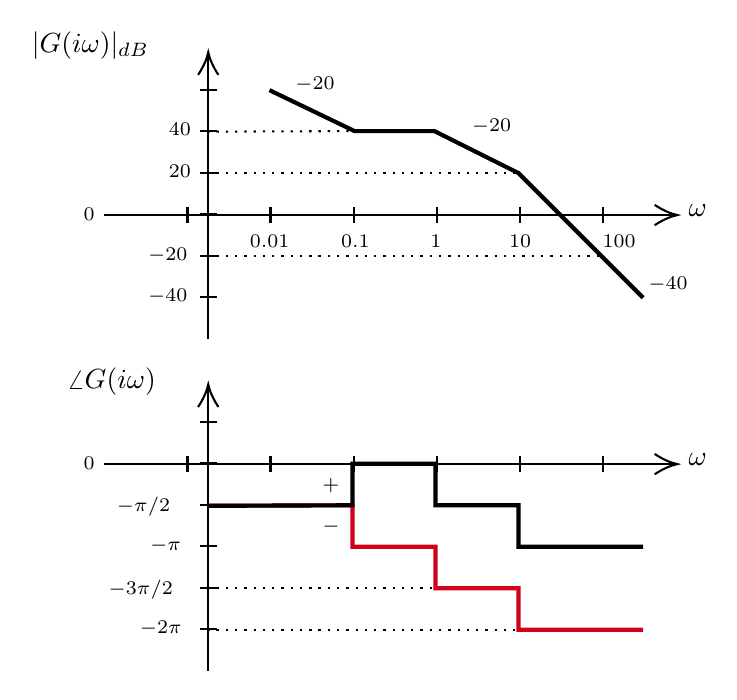
\begin{tikzpicture}[x=0.75pt,y=0.75pt,yscale=-1,xscale=1]
		%uncomment if require: \path (0,343); %set diagram left start at 0, and has height of 343
		
		\draw [line width=1.5]    (160,50) -- (201,69.73) -- (239.5,69.73) -- (280,90) -- (340,150) ;
		\draw    (80.5,110.18) -- (354.5,110.18) (120.5,106.18) -- (120.5,114.18)(160.5,106.18) -- (160.5,114.18)(200.5,106.18) -- (200.5,114.18)(240.5,106.18) -- (240.5,114.18)(280.5,106.18) -- (280.5,114.18)(320.5,106.18) -- (320.5,114.18) ;
		\draw [shift={(356.5,110.18)}, rotate = 180] [color={rgb, 255:red, 0; green, 0; blue, 0 }  ][line width=0.75]    (10.93,-4.9) .. controls (6.95,-2.3) and (3.31,-0.67) .. (0,0) .. controls (3.31,0.67) and (6.95,2.3) .. (10.93,4.9)   ;
		\draw    (130.5,169.73) -- (130.5,33.73) (126.5,149.73) -- (134.5,149.73)(126.5,129.73) -- (134.5,129.73)(126.5,109.73) -- (134.5,109.73)(126.5,89.73) -- (134.5,89.73)(126.5,69.73) -- (134.5,69.73)(126.5,49.73) -- (134.5,49.73) ;
		\draw [shift={(130.5,31.73)}, rotate = 450] [color={rgb, 255:red, 0; green, 0; blue, 0 }  ][line width=0.75]    (10.93,-4.9) .. controls (6.95,-2.3) and (3.31,-0.67) .. (0,0) .. controls (3.31,0.67) and (6.95,2.3) .. (10.93,4.9)   ;
		\draw  [dash pattern={on 0.84pt off 2.51pt}]  (130,90) -- (280,90) ;
		\draw  [dash pattern={on 0.84pt off 2.51pt}]  (130,70) -- (201,69.73) ;
		\draw  [dash pattern={on 0.84pt off 2.51pt}]  (130,130) -- (320,130) ;
		\draw    (80.5,230.18) -- (354.5,230.18) (120.5,226.18) -- (120.5,234.18)(160.5,226.18) -- (160.5,234.18)(200.5,226.18) -- (200.5,234.18)(240.5,226.18) -- (240.5,234.18)(280.5,226.18) -- (280.5,234.18)(320.5,226.18) -- (320.5,234.18) ;
		\draw [shift={(356.5,230.18)}, rotate = 180] [color={rgb, 255:red, 0; green, 0; blue, 0 }  ][line width=0.75]    (10.93,-4.9) .. controls (6.95,-2.3) and (3.31,-0.67) .. (0,0) .. controls (3.31,0.67) and (6.95,2.3) .. (10.93,4.9)   ;
		\draw    (130.5,329.73) -- (130.5,193.73) (126.5,309.73) -- (134.5,309.73)(126.5,289.73) -- (134.5,289.73)(126.5,269.73) -- (134.5,269.73)(126.5,249.73) -- (134.5,249.73)(126.5,229.73) -- (134.5,229.73)(126.5,209.73) -- (134.5,209.73) ;
		\draw [shift={(130.5,191.73)}, rotate = 450] [color={rgb, 255:red, 0; green, 0; blue, 0 }  ][line width=0.75]    (10.93,-4.9) .. controls (6.95,-2.3) and (3.31,-0.67) .. (0,0) .. controls (3.31,0.67) and (6.95,2.3) .. (10.93,4.9)   ;
		\draw [color={rgb, 255:red, 208; green, 2; blue, 27 }  ,draw opacity=1 ][line width=1.5]    (130.5,250.27) -- (200,250) -- (200,270) -- (240,270) -- (240,290) -- (280,290) -- (280,310) -- (340,310) ;
		\draw [line width=1.5]    (130.5,250.27) -- (200,250) -- (200,230) -- (240,230) -- (240,250) -- (280,250) -- (280,270) -- (340,270) ;
		\draw  [dash pattern={on 0.84pt off 2.51pt}]  (130,310) -- (280,310) ;
		\draw  [dash pattern={on 0.84pt off 2.51pt}]  (130,290) -- (240,290) ;
		
		\draw (360.5,103.58) node [anchor=north west][inner sep=0.75pt]    {$\omega $};
		\draw (44,20.4) node [anchor=north west][inner sep=0.75pt]    {$| G(i\omega)| _{\si{dB}}$};
		\draw (236,118.4) node [anchor=north west][inner sep=0.75pt]  [font=\scriptsize]  {$1$};
		\draw (274,118.4) node [anchor=north west][inner sep=0.75pt]  [font=\scriptsize]  {$10$};
		\draw (319,118.4) node [anchor=north west][inner sep=0.75pt]  [font=\scriptsize]  {$100$};
		\draw (193,118.4) node [anchor=north west][inner sep=0.75pt]  [font=\scriptsize]  {$0.1$};
		\draw (69,105.4) node [anchor=north west][inner sep=0.75pt]  [font=\scriptsize]  {$0$};
		\draw (110,84.4) node [anchor=north west][inner sep=0.75pt]  [font=\scriptsize]  {$20$};
		\draw (110,64.4) node [anchor=north west][inner sep=0.75pt]  [font=\scriptsize]  {$40$};
		\draw (100,124.4) node [anchor=north west][inner sep=0.75pt]  [font=\scriptsize]  {$-20$};
		\draw (100,144.4) node [anchor=north west][inner sep=0.75pt]  [font=\scriptsize]  {$-40$};
		\draw (149,118.4) node [anchor=north west][inner sep=0.75pt]  [font=\scriptsize]  {$0.01$};
		\draw (171,42.4) node [anchor=north west][inner sep=0.75pt]  [font=\scriptsize]  {$-20$};
		\draw (256,62.4) node [anchor=north west][inner sep=0.75pt]  [font=\scriptsize]  {$-20$};
		\draw (341,138.4) node [anchor=north west][inner sep=0.75pt]  [font=\scriptsize]  {$-40$};
		\draw (360.5,223.58) node [anchor=north west][inner sep=0.75pt]    {$\omega $};
		\draw (61,182.4) node [anchor=north west][inner sep=0.75pt]    {$\angle G(i\omega)$};
		\draw (69,225.4) node [anchor=north west][inner sep=0.75pt]  [font=\scriptsize]  {$0$};
		\draw (85,244.4) node [anchor=north west][inner sep=0.75pt]  [font=\scriptsize]  {$-\pi /2$};
		\draw (101,264.4) node [anchor=north west][inner sep=0.75pt]  [font=\scriptsize]  {$-\pi $};
		\draw (81,284.4) node [anchor=north west][inner sep=0.75pt]  [font=\scriptsize]  {$-3\pi /2$};
		\draw (96,304.4) node [anchor=north west][inner sep=0.75pt]  [font=\scriptsize]  {$-2\pi $};
		\draw (184,235.4) node [anchor=north west][inner sep=0.75pt]  [font=\scriptsize]  {$+$};
		\draw (184,255.4) node [anchor=north west][inner sep=0.75pt]  [font=\scriptsize]  {$-$};
		
		
	\end{tikzpicture}
\end{figure}\FloatBarrier

Il diagramma di Bode del modulo non basta per realizzare la funzione di trasferimento, lascia incertezze sulle costanti di tempo. Serve o l'informazione sulla fase o qualche altra informazione, anche minimale, per escludere le ambiguità.

In realtà ne esistono infinite che hanno lo stesso diagramma, basta considerare una
\begin{equation*}
	\tilde{G}(s) =G(s) \cdotp \frac{1-s\tau }{1+s\tau }
\end{equation*}
Il secondo oggetto si chiama \textbf{sfasatore puro}. Sul modulo non cambia niente, ma sfasa la fase di $-\pi $, concentrato in $\frac{1}{| \tau | }$.

\section{Poli complessi coniugati}

Supponiamo $\mu =1$ e scriviamo la $G(s)$ come
\begin{equation*}
	G(s) =\frac{\omega ^2_n}{s^2 +2\xi \omega _n s+\omega ^2_n}
\end{equation*}
Ricordiamo che per avere stabilità e poli complessi coniugati dobbiamo avere
\begin{equation*}
	0< \xi < 1\ \ \implies \ \ p_{1,2} =-\omega _n \xi \pm i\omega _n\sqrt{1-\xi ^2}
\end{equation*}
$G(i\omega)$ possiamo scriverla in forma normalizzata
\begin{equation*}
	G(i\omega) =\frac{\omega ^2_n}{-\omega ^2 +i2\xi \omega _n \omega +\omega ^2_n} =\frac{1}{\left[ 1-\left(\frac{\omega }{\omega _n}\right)^2\right] +i\left[ 2\xi \frac{\omega }{\omega _n}\right]}
\end{equation*}
Scriviamo il modulo
\begin{equation*}
	| G(i\omega)| =\frac{1}{\sqrt{\left[ 1-\left(\frac{\omega }{\omega _n}\right)^2\right]^2 +\left[ 2\xi \frac{\omega }{\omega _n}\right]^2}}
\end{equation*}
Ci accorgiamo che si forma un massimo per $\xi < \frac{1}{\sqrt{2}} \approx 0,707$ e il massimo ha valore $| G(i\omega _{\text{max}})| =\frac{1}{2\xi \sqrt{1-\xi ^2}}$ in corrispondenza di $\omega _{\text{max}} =\omega _n\sqrt{1-2\xi ^2}$

\begin{figure}[htpb]\centering
	\tikzset{every picture/.style={line width=0.75pt}} %set default line width to 0.75pt        
	
	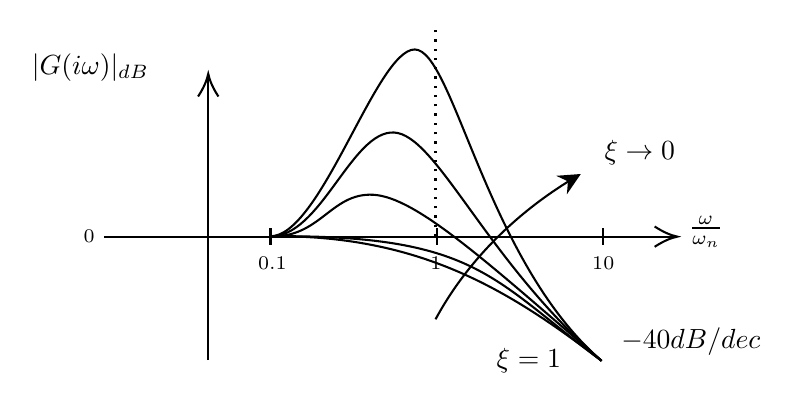
\begin{tikzpicture}[x=0.75pt,y=0.75pt,yscale=-1,xscale=1]
		%uncomment if require: \path (0,198); %set diagram left start at 0, and has height of 198
		
		\draw    (100.5,120.18) -- (374.5,120.18) (180.5,116.18) -- (180.5,124.18)(260.5,116.18) -- (260.5,124.18)(340.5,116.18) -- (340.5,124.18) ;
		\draw [shift={(376.5,120.18)}, rotate = 180] [color={rgb, 255:red, 0; green, 0; blue, 0 }  ][line width=0.75]    (10.93,-4.9) .. controls (6.95,-2.3) and (3.31,-0.67) .. (0,0) .. controls (3.31,0.67) and (6.95,2.3) .. (10.93,4.9)   ;
		\draw    (150.5,179.73) -- (150.5,43.73) ;
		\draw [shift={(150.5,41.73)}, rotate = 450] [color={rgb, 255:red, 0; green, 0; blue, 0 }  ][line width=0.75]    (10.93,-4.9) .. controls (6.95,-2.3) and (3.31,-0.67) .. (0,0) .. controls (3.31,0.67) and (6.95,2.3) .. (10.93,4.9)   ;
		%Curve Lines [id:da19724670089989216] 
		\draw    (180,120) .. controls (251.5,119.08) and (294.5,145.08) .. (340,180) ;
		%Curve Lines [id:da5465409433450557] 
		\draw    (180,120) .. controls (279.5,119.08) and (286.5,140.08) .. (340,180) ;
		%Curve Lines [id:da5442911027612884] 
		\draw    (180,120) .. controls (204.5,121.08) and (209.5,98.92) .. (230,100) .. controls (250.5,101.08) and (284.5,132.08) .. (340,180) ;
		%Curve Lines [id:da8374002820306299] 
		\draw    (180,120) .. controls (204.5,121.08) and (219.5,68.92) .. (240,70) .. controls (260.5,71.08) and (284.5,132.08) .. (340,180) ;
		%Curve Lines [id:da2687067168629047] 
		\draw    (180,120) .. controls (204.5,121.08) and (231.5,29.92) .. (250,30) .. controls (268.5,30.08) and (284.5,132.08) .. (340,180) ;
		\draw  [dash pattern={on 0.84pt off 2.51pt}]  (260,120) -- (260,20) ;
		%Curve Lines [id:da1670752414310075] 
		\draw    (260,160) .. controls (274.14,133.75) and (297.31,109.33) .. (327.65,91.37) ;
		\draw [shift={(330,90)}, rotate = 510.15] [fill={rgb, 255:red, 0; green, 0; blue, 0 }  ][line width=0.08]  [draw opacity=0] (10.72,-5.15) -- (0,0) -- (10.72,5.15) -- (7.12,0) -- cycle    ;
		
		\draw (380.5,108.58) node [anchor=north west][inner sep=0.75pt]    {$\frac{\omega }{\omega _n}$};
		\draw (64,30.4) node [anchor=north west][inner sep=0.75pt]    {$| G(i\omega)| _{\si{dB}}$};
		\draw (256,128.4) node [anchor=north west][inner sep=0.75pt]  [font=\scriptsize]  {$1$};
		\draw (334,128.4) node [anchor=north west][inner sep=0.75pt]  [font=\scriptsize]  {$10$};
		\draw (173,128.4) node [anchor=north west][inner sep=0.75pt]  [font=\scriptsize]  {$0.1$};
		\draw (89,115.4) node [anchor=north west][inner sep=0.75pt]  [font=\scriptsize]  {$0$};
		\draw (340,72.4) node [anchor=north west][inner sep=0.75pt]    {$\xi \to 0$};
		\draw (288,172.4) node [anchor=north west][inner sep=0.75pt]    {$\xi =1$};
		\draw (348,162.4) node [anchor=north west][inner sep=0.75pt]    {$-40\si{dB/dec}$};
		
		
	\end{tikzpicture}
\end{figure}\FloatBarrier

Questo fenomeno si chiama \textbf{risonanza}.

L'argomento invece vale
\begin{equation*}
	\arg G(i\omega) =-\arctan\left[\left(2\xi \frac{\omega }{\omega _n}\right) /\left(1-\left(\frac{\omega }{\omega _n}\right)^2\right)\right]
\end{equation*}

\begin{figure}[htpb]\centering
	\tikzset{every picture/.style={line width=0.75pt}} %set default line width to 0.75pt        
	
	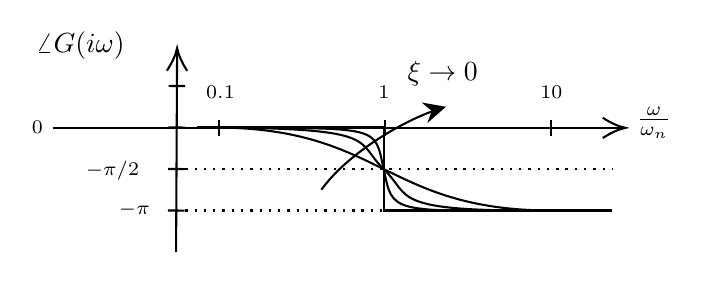
\begin{tikzpicture}[x=0.75pt,y=0.75pt,yscale=-1,xscale=1]
		%uncomment if require: \path (0,141); %set diagram left start at 0, and has height of 141
		
		\draw    (180,130) -- (180.49,33.73) (176.1,109.98) -- (184.1,110.02)(176.2,89.98) -- (184.2,90.02)(176.31,69.98) -- (184.31,70.02)(176.41,49.98) -- (184.41,50.02) ;
		\draw [shift={(180.5,31.73)}, rotate = 450.29] [color={rgb, 255:red, 0; green, 0; blue, 0 }  ][line width=0.75]    (10.93,-4.9) .. controls (6.95,-2.3) and (3.31,-0.67) .. (0,0) .. controls (3.31,0.67) and (6.95,2.3) .. (10.93,4.9)   ;
		\draw [line width=0.75]    (190,70) -- (280,70) -- (280,110) -- (390,110) ;
		\draw  [dash pattern={on 0.84pt off 2.51pt}]  (180,90) -- (390,90) ;
		\draw  [dash pattern={on 0.84pt off 2.51pt}]  (180,110) -- (280,110) ;
		\draw    (120.5,70.18) -- (394.5,70.18) (200.5,66.18) -- (200.5,74.18)(280.5,66.18) -- (280.5,74.18)(360.5,66.18) -- (360.5,74.18) ;
		\draw [shift={(396.5,70.18)}, rotate = 180] [color={rgb, 255:red, 0; green, 0; blue, 0 }  ][line width=0.75]    (10.93,-4.9) .. controls (6.95,-2.3) and (3.31,-0.67) .. (0,0) .. controls (3.31,0.67) and (6.95,2.3) .. (10.93,4.9)   ;
		%Curve Lines [id:da7484005914366461] 
		\draw    (200,70) .. controls (279.5,70.52) and (280.5,109.52) .. (360,110) ;
		%Curve Lines [id:da523489403125242] 
		\draw    (200,70) .. controls (279.5,70.52) and (266,76.5) .. (280,90) .. controls (294,103.5) and (281.5,110.52) .. (360,110) ;
		%Curve Lines [id:da784046407935008] 
		\draw    (200,70) .. controls (279.5,70.52) and (275.33,68.83) .. (280,90) .. controls (284.67,111.17) and (281.5,110.52) .. (360,110) ;
		%Curve Lines [id:da5893091681194245] 
		\draw    (250,100) .. controls (261.94,83.3) and (288.01,67.05) .. (307.32,60.81) ;
		\draw [shift={(310,60)}, rotate = 524.21] [fill={rgb, 255:red, 0; green, 0; blue, 0 }  ][line width=0.08]  [draw opacity=0] (10.72,-5.15) -- (0,0) -- (10.72,5.15) -- (7.12,0) -- cycle    ;
		
		\draw (111,22.4) node [anchor=north west][inner sep=0.75pt]    {$\angle G(i\omega)$};
		\draw (135,84.4) node [anchor=north west][inner sep=0.75pt]  [font=\scriptsize]  {$-\pi /2$};
		\draw (151,104.4) node [anchor=north west][inner sep=0.75pt]  [font=\scriptsize]  {$-\pi $};
		\draw (400.5,58.58) node [anchor=north west][inner sep=0.75pt]    {$\frac{\omega }{\omega _n}$};
		\draw (276,48.4) node [anchor=north west][inner sep=0.75pt]  [font=\scriptsize]  {$1$};
		\draw (354,48.4) node [anchor=north west][inner sep=0.75pt]  [font=\scriptsize]  {$10$};
		\draw (193,48.4) node [anchor=north west][inner sep=0.75pt]  [font=\scriptsize]  {$0.1$};
		\draw (109,65.4) node [anchor=north west][inner sep=0.75pt]  [font=\scriptsize]  {$0$};
		\draw (290,36.4) node [anchor=north west][inner sep=0.75pt]    {$\xi \to 0$};
		
		
	\end{tikzpicture}
\end{figure}\FloatBarrier

Nello studio di queste funzioni di trasferimento è importante mettere in evidenza il termine $\omega ^2_n$ a numeratore per valutare correttamente il $\mu $ del sistema, cercando la cosiddetta \textbf{forma standard}, in modo che il termine non influisca prima della sua frequenza caratteristica $\omega _n$
\begin{equation*}
	\boxed{G(s) =\frac{\mu }{s^h} \cdot \frac{\prod _j(1+s\tau _j)}{\prod _j(1+sT_j)} \cdot \frac{\omega ^2_n}{s^2 +2\xi \omega _n s+\omega ^2_n}}
\end{equation*}
\textit{Esempio.}
\begin{equation*}
	G(s) =\frac{10^3 s}{(1+s)\left(s^2 +s+100\right)} =10s\cdot \frac{1}{1+s} \cdot \frac{100}{s^2 +s+100}
\end{equation*}
pertanto ricaviamo i valori della \textbf{pulsazione naturale} $\omega _n$ e dello \textbf{smorzamento} $\xi $
\begin{gather*}
	\omega ^2_n =100\ \ \implies \ \ \omega _n =10\\
	2\xi \omega _n =1\ \ \implies \ \ \xi =\frac{1}{20} =0.05
\end{gather*}
Alle basse frequenze abbiamo che il tipo è $h=-1$, quindi saliamo di $+20\ \si{dB/dec}$, mentre per $\omega =1$ deve valere $10$, cioè $20\ \si{dB}$. Alla frequenza $\omega =1$ interviene un polo. Alla frequenza $\omega =10$ interviene la coppia di poli facendo scendere di $-40\ \si{dB/dec}$. Questa conferma si ha dal fatto che $r=2$.

Per assicurarci che in $\omega =10$ ci sia risonanza, calcoliamo l'incremento
\begin{equation*}
	\frac{1}{2\xi \sqrt{1-\xi ^2}} =\frac{1}{2(0.05)\sqrt{1-(0.05)^2}} \approx \frac{1}{2(0.05)} =10=20\ \si{dB}
\end{equation*}
Ciò significa che in realtà il diagramma si trova $20\ \si{dB}$ più in alto rispetto a ciò che abbiamo disegnato nel diagramma di Bode.

Essendo inoltre $\xi $ molto prossimo a $0$, il diagramma reale della fase sarà prossimo alla discontinuità.

\begin{figure}[htpb]
	\centering
	\tikzset{every picture/.style={line width=0.75pt}} %set default line width to 0.75pt        
	
	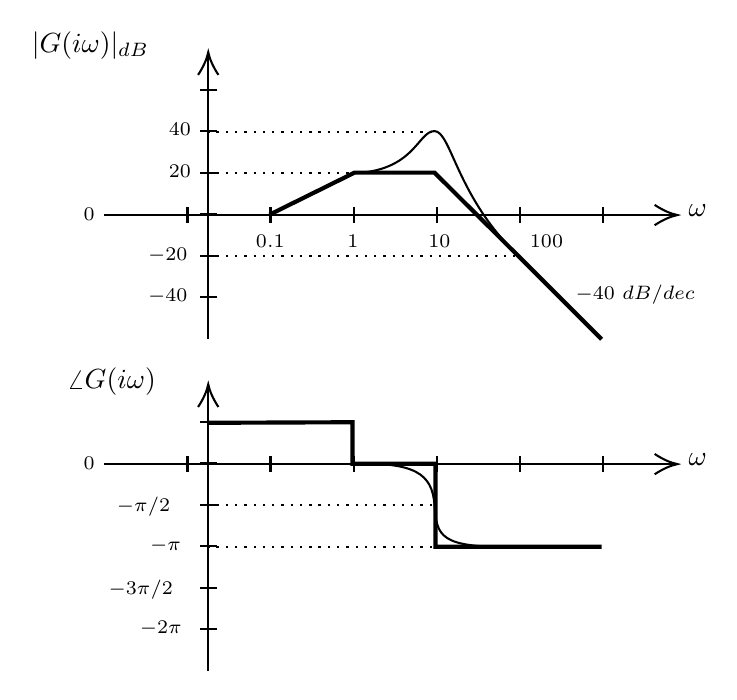
\begin{tikzpicture}[x=0.75pt,y=0.75pt,yscale=-1,xscale=1]
		%uncomment if require: \path (0,343); %set diagram left start at 0, and has height of 343
		
		
		\draw [line width=1.5]    (160,110) -- (201,89.73) -- (239.5,89.73) -- (280,130) -- (320,170) ;
		
		\draw    (80.5,110.18) -- (354.5,110.18) (120.5,106.18) -- (120.5,114.18)(160.5,106.18) -- (160.5,114.18)(200.5,106.18) -- (200.5,114.18)(240.5,106.18) -- (240.5,114.18)(280.5,106.18) -- (280.5,114.18)(320.5,106.18) -- (320.5,114.18) ;
		\draw [shift={(356.5,110.18)}, rotate = 180] [color={rgb, 255:red, 0; green, 0; blue, 0 }  ][line width=0.75]    (10.93,-4.9) .. controls (6.95,-2.3) and (3.31,-0.67) .. (0,0) .. controls (3.31,0.67) and (6.95,2.3) .. (10.93,4.9)   ;
		
		\draw    (130.5,169.73) -- (130.5,33.73) (126.5,149.73) -- (134.5,149.73)(126.5,129.73) -- (134.5,129.73)(126.5,109.73) -- (134.5,109.73)(126.5,89.73) -- (134.5,89.73)(126.5,69.73) -- (134.5,69.73)(126.5,49.73) -- (134.5,49.73) ;
		\draw [shift={(130.5,31.73)}, rotate = 450] [color={rgb, 255:red, 0; green, 0; blue, 0 }  ][line width=0.75]    (10.93,-4.9) .. controls (6.95,-2.3) and (3.31,-0.67) .. (0,0) .. controls (3.31,0.67) and (6.95,2.3) .. (10.93,4.9)   ;
		
		\draw  [dash pattern={on 0.84pt off 2.51pt}]  (130,90) -- (200,90) ;
		
		\draw  [dash pattern={on 0.84pt off 2.51pt}]  (130,130) -- (280,130) ;
		
		\draw    (80.5,230.18) -- (354.5,230.18) (120.5,226.18) -- (120.5,234.18)(160.5,226.18) -- (160.5,234.18)(200.5,226.18) -- (200.5,234.18)(240.5,226.18) -- (240.5,234.18)(280.5,226.18) -- (280.5,234.18)(320.5,226.18) -- (320.5,234.18) ;
		\draw [shift={(356.5,230.18)}, rotate = 180] [color={rgb, 255:red, 0; green, 0; blue, 0 }  ][line width=0.75]    (10.93,-4.9) .. controls (6.95,-2.3) and (3.31,-0.67) .. (0,0) .. controls (3.31,0.67) and (6.95,2.3) .. (10.93,4.9)   ;
		
		\draw    (130.5,329.73) -- (130.5,193.73) (126.5,309.73) -- (134.5,309.73)(126.5,289.73) -- (134.5,289.73)(126.5,269.73) -- (134.5,269.73)(126.5,249.73) -- (134.5,249.73)(126.5,229.73) -- (134.5,229.73)(126.5,209.73) -- (134.5,209.73) ;
		\draw [shift={(130.5,191.73)}, rotate = 450] [color={rgb, 255:red, 0; green, 0; blue, 0 }  ][line width=0.75]    (10.93,-4.9) .. controls (6.95,-2.3) and (3.31,-0.67) .. (0,0) .. controls (3.31,0.67) and (6.95,2.3) .. (10.93,4.9)   ;
		
		\draw [line width=1.5]    (130.5,210.27) -- (200,210) -- (200,230) -- (240,230) -- (240,270) -- (320,270) ;
		
		\draw  [dash pattern={on 0.84pt off 2.51pt}]  (130,250) -- (240,250) ;
		
		\draw  [dash pattern={on 0.84pt off 2.51pt}]  (130,270) -- (240,270) ;
		%Curve Lines [id:da873427168956133] 
		\draw    (200,90) .. controls (230,89.25) and (231.5,69.67) .. (239.5,69.73) .. controls (247.5,69.8) and (250,101.25) .. (280,130) ;
		
		\draw  [dash pattern={on 0.84pt off 2.51pt}]  (130,70) -- (240,70) ;
		%Curve Lines [id:da2393030512935308] 
		\draw    (200,230) .. controls (230,229.25) and (238.33,234.64) .. (239.5,249.73) .. controls (240.67,264.83) and (241.33,270.83) .. (280,270) ;
		
		
		\draw (360.5,103.58) node [anchor=north west][inner sep=0.75pt]    {$\omega $};
		
		\draw (44,20.4) node [anchor=north west][inner sep=0.75pt]    {$| G(i\omega)| _{\si{dB}}$};
		
		\draw (235,118.4) node [anchor=north west][inner sep=0.75pt]  [font=\scriptsize]  {$10$};
		
		\draw (284,118.4) node [anchor=north west][inner sep=0.75pt]  [font=\scriptsize]  {$100$};
		
		\draw (196,118.4) node [anchor=north west][inner sep=0.75pt]  [font=\scriptsize]  {$1$};
		
		\draw (69,105.4) node [anchor=north west][inner sep=0.75pt]  [font=\scriptsize]  {$0$};
		
		\draw (110,84.4) node [anchor=north west][inner sep=0.75pt]  [font=\scriptsize]  {$20$};
		
		\draw (110,64.4) node [anchor=north west][inner sep=0.75pt]  [font=\scriptsize]  {$40$};
		
		\draw (100,124.4) node [anchor=north west][inner sep=0.75pt]  [font=\scriptsize]  {$-20$};
		
		\draw (100,144.4) node [anchor=north west][inner sep=0.75pt]  [font=\scriptsize]  {$-40$};
		
		\draw (152,118.4) node [anchor=north west][inner sep=0.75pt]  [font=\scriptsize]  {$0.1$};
		
		\draw (306,142.4) node [anchor=north west][inner sep=0.75pt]  [font=\scriptsize]  {$-40\ \si{dB/dec}$};
		
		\draw (360.5,223.58) node [anchor=north west][inner sep=0.75pt]    {$\omega $};
		
		\draw (61,182.4) node [anchor=north west][inner sep=0.75pt]    {$\angle G(i\omega)$};
		
		\draw (69,225.4) node [anchor=north west][inner sep=0.75pt]  [font=\scriptsize]  {$0$};
		
		\draw (85,244.4) node [anchor=north west][inner sep=0.75pt]  [font=\scriptsize]  {$-\pi /2$};
		
		\draw (101,264.4) node [anchor=north west][inner sep=0.75pt]  [font=\scriptsize]  {$-\pi $};
		
		\draw (81,284.4) node [anchor=north west][inner sep=0.75pt]  [font=\scriptsize]  {$-3\pi /2$};
		
		\draw (96,304.4) node [anchor=north west][inner sep=0.75pt]  [font=\scriptsize]  {$-2\pi $};
		
		
	\end{tikzpicture}
\end{figure}
\FloatBarrier

Nel caso di \textbf{zeri complessi coniugati}, si ha la situazione opposta
\begin{equation*}
	G(s) =\frac{\mu }{s^h} \cdot \frac{\prod _j(1+s\tau _j)}{\prod _j(1+sT_j)} \cdot \frac{s^2 +2\xi \omega _n s+\omega ^2_n}{\omega ^2_n}
\end{equation*}
Anche qui è importante studiare la forma standard. Nei diagrammi si ritrova lo stesso discorso, simmetrico rispetto all'asse delle ascisse.

\chapter{Sistemi di controllo}

Se il guadagno è ben definito e non nullo, allora
\begin{equation*}
	\overline{y} =G(0)\overline{u}
\end{equation*}
C'è un problema, affinché $y(t)\implies \overline{y}$ serve che $G(s)$ sia asintoticamente stabile, ma la $G(s)$ reale è in generale diversa dalla $\tilde{G}(s)$ approssimata del modello. Quindi usiamo sistemi in \textbf{retroazione}.

La differenza tra il valore desiderato di $y$ e la $y(t)$ va a zero? La retroazione, come sappiamo, può non mantenere la stabilità. Chiamiamo $w(t)$ l'uscita desiderata, $e(t)$ l'errore commesso e $d(t)$ un eventuale disturbo in uscita.

\begin{figure}[htpb]\centering
	\tikzset{every picture/.style={line width=0.75pt}} %set default line width to 0.75pt        
	
	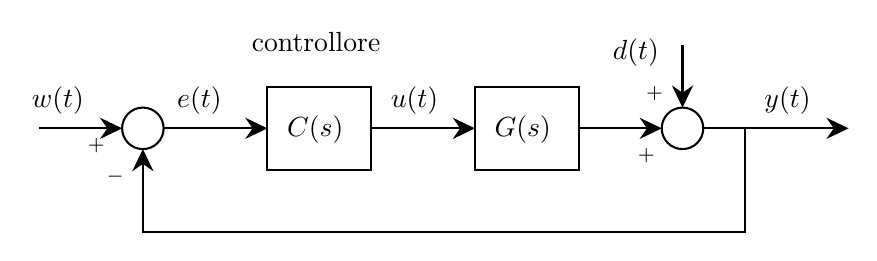
\begin{tikzpicture}[x=0.75pt,y=0.75pt,yscale=-1,xscale=1]
		%uncomment if require: \path (0,121); %set diagram left start at 0, and has height of 121
		
		%Shape: Circle [id:dp4465774216142955] 
		\draw   (110,60) .. controls (110,54.48) and (114.48,50) .. (120,50) .. controls (125.52,50) and (130,54.48) .. (130,60) .. controls (130,65.52) and (125.52,70) .. (120,70) .. controls (114.48,70) and (110,65.52) .. (110,60) -- cycle ;
		\draw    (70,60) -- (107,60) ;
		\draw [shift={(110,60)}, rotate = 180] [fill={rgb, 255:red, 0; green, 0; blue, 0 }  ][line width=0.08]  [draw opacity=0] (10.72,-5.15) -- (0,0) -- (10.72,5.15) -- (7.12,0) -- cycle    ;
		\draw    (130,60) -- (177,60) ;
		\draw [shift={(180,60)}, rotate = 180] [fill={rgb, 255:red, 0; green, 0; blue, 0 }  ][line width=0.08]  [draw opacity=0] (10.72,-5.15) -- (0,0) -- (10.72,5.15) -- (7.12,0) -- cycle    ;
		%Shape: Rectangle [id:dp3937243862126707] 
		\draw   (180,40) -- (230,40) -- (230,80) -- (180,80) -- cycle ;
		%Shape: Rectangle [id:dp4020437611981835] 
		\draw   (280,40) -- (330,40) -- (330,80) -- (280,80) -- cycle ;
		\draw    (230,60) -- (277,60) ;
		\draw [shift={(280,60)}, rotate = 180] [fill={rgb, 255:red, 0; green, 0; blue, 0 }  ][line width=0.08]  [draw opacity=0] (10.72,-5.15) -- (0,0) -- (10.72,5.15) -- (7.12,0) -- cycle    ;
		%Shape: Circle [id:dp4212750993239298] 
		\draw   (370,60) .. controls (370,54.48) and (374.48,50) .. (380,50) .. controls (385.52,50) and (390,54.48) .. (390,60) .. controls (390,65.52) and (385.52,70) .. (380,70) .. controls (374.48,70) and (370,65.52) .. (370,60) -- cycle ;
		\draw    (330,60) -- (367,60) ;
		\draw [shift={(370,60)}, rotate = 180] [fill={rgb, 255:red, 0; green, 0; blue, 0 }  ][line width=0.08]  [draw opacity=0] (10.72,-5.15) -- (0,0) -- (10.72,5.15) -- (7.12,0) -- cycle    ;
		\draw    (390,60) -- (457,60) ;
		\draw [shift={(460,60)}, rotate = 180] [fill={rgb, 255:red, 0; green, 0; blue, 0 }  ][line width=0.08]  [draw opacity=0] (10.72,-5.15) -- (0,0) -- (10.72,5.15) -- (7.12,0) -- cycle    ;
		\draw    (410,60) -- (410,110) -- (120,110) -- (120,73) ;
		\draw [shift={(120,70)}, rotate = 450] [fill={rgb, 255:red, 0; green, 0; blue, 0 }  ][line width=0.08]  [draw opacity=0] (10.72,-5.15) -- (0,0) -- (10.72,5.15) -- (7.12,0) -- cycle    ;
		\draw    (380,20) -- (380,47) ;
		\draw [shift={(380,50)}, rotate = 270] [fill={rgb, 255:red, 0; green, 0; blue, 0 }  ][line width=0.08]  [draw opacity=0] (10.72,-5.15) -- (0,0) -- (10.72,5.15) -- (7.12,0) -- cycle    ;
		
		\draw (188,52.4) node [anchor=north west][inner sep=0.75pt]    {$C(s)$};
		\draw (288,52.4) node [anchor=north west][inner sep=0.75pt]    {$G(s)$};
		\draw (65,38.4) node [anchor=north west][inner sep=0.75pt]    {$w(t)$};
		\draw (135,38.4) node [anchor=north west][inner sep=0.75pt]    {$e(t)$};
		\draw (238,38.4) node [anchor=north west][inner sep=0.75pt]    {$u(t)$};
		\draw (345,15.4) node [anchor=north west][inner sep=0.75pt]    {$d(t)$};
		\draw (418,38.4) node [anchor=north west][inner sep=0.75pt]    {$y(t)$};
		\draw (92,63.4) node [anchor=north west][inner sep=0.75pt]  [font=\scriptsize]  {$+$};
		\draw (101,78.4) node [anchor=north west][inner sep=0.75pt]  [font=\scriptsize]  {$-$};
		\draw (357,68.4) node [anchor=north west][inner sep=0.75pt]  [font=\scriptsize]  {$+$};
		\draw (361,38.4) node [anchor=north west][inner sep=0.75pt]  [font=\scriptsize]  {$+$};
		\draw (171,12) node [anchor=north west][inner sep=0.75pt]   [align=left] {controllore};
		
		
	\end{tikzpicture}
\end{figure}\FloatBarrier

\begin{equation*}
	\begin{aligned}
		y       & =d+CGe     \\
		        & =d+CG(w-y) \\
		y(1+CG) & =d+CGw     
	\end{aligned} \ \ \implies \ \ y=\frac{1}{1+CG} d+\frac{CG}{1+CG} w
\end{equation*}
Definiamo la \textbf{funzione di trasferimento d'anello}
\begin{equation*}
	\boxed{L(s) =C(s) G(s)}
\end{equation*}
Allora possiamo descrivere l'uscita come
\begin{equation*}
	y=\frac{1}{1+L} d+\frac{L}{1+L} w
\end{equation*}
E analogamente possiamo anche descrivere l'errore come
\begin{equation*}
	\begin{aligned}
		e      & =w-y      \\
		       & =w-(d+Le) \\
		e(1+L) & =w-d      
	\end{aligned} \ \ \implies \ \ e=\frac{1}{1+L} w-\frac{1}{1+L} d
\end{equation*}
In base alla grandezza che vorremo descrivere (errore o uscita di solito) e agli elementi che lo influenzano, vari tipi di disturbi che vedremo più avanti, avremo diverse funzioni di $L$.

\textbf{Requisiti di un sistema di controllo:}
\begin{itemize}
	\item stabilità asintotica
	\item stabilità robusta (stabile per $G$ vicine a quella vera)
	\item velocità di risposta elevata
	\item parsimonia di $u(t)$
	\item attenuazione dei disturbi
	\item piccolo errore a regime
\end{itemize}

\section{Stabilità asintotica}

Non dobbiamo studiare $L$ ma $H(s) =\frac{L(s)}{1+L(s)}$. Usiamo il \textbf{criterio di Bode}. Immaginiamo $L(s)$ propria e
\begin{itemize}
	\item $\Re(p_i) \leq 0\ \forall i$ (poli di $L(s)$)
	\item $| L(i\omega)| $ attraversa $0\ \si{dB}$ una sola volta in $\omega =\omega _c$ (quindi per forza dall'alto verso il basso)
\end{itemize}

Allora $H(s)$ è asint. stabile se e solo se
\begin{itemize}
	\item $\mu  >0$
	\item $\varphi _m  >0$, dove $\varphi _m$ è il \textbf{margine di fase} e vale $\varphi _m =\pi -| \varphi _c| $, dove $\varphi _c$ è la \textbf{fase critica} e vale $\varphi _c =\arg L(i\omega _c)$
	      \begin{itemize}
	      	\item ovvero se $| \varphi _c| < \pi $
	      \end{itemize}
\end{itemize}

\section{Banda passante e tempo di risposta}

Consideriamo un semplice sistema di controllo

\begin{figure}[htpb]\centering
	\tikzset{every picture/.style={line width=0.75pt}} %set default line width to 0.75pt        
	
	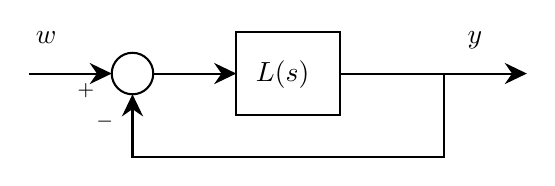
\begin{tikzpicture}[x=0.75pt,y=0.75pt,yscale=-1,xscale=1]
		%uncomment if require: \path (0,88); %set diagram left start at 0, and has height of 88
		
		%Shape: Circle [id:dp22706009120032955] 
		\draw   (200,40) .. controls (200,34.48) and (204.48,30) .. (210,30) .. controls (215.52,30) and (220,34.48) .. (220,40) .. controls (220,45.52) and (215.52,50) .. (210,50) .. controls (204.48,50) and (200,45.52) .. (200,40) -- cycle ;
		\draw    (160,40) -- (197,40) ;
		\draw [shift={(200,40)}, rotate = 180] [fill={rgb, 255:red, 0; green, 0; blue, 0 }  ][line width=0.08]  [draw opacity=0] (10.72,-5.15) -- (0,0) -- (10.72,5.15) -- (7.12,0) -- cycle    ;
		\draw    (220,40) -- (257,40) ;
		\draw [shift={(260,40)}, rotate = 180] [fill={rgb, 255:red, 0; green, 0; blue, 0 }  ][line width=0.08]  [draw opacity=0] (10.72,-5.15) -- (0,0) -- (10.72,5.15) -- (7.12,0) -- cycle    ;
		%Shape: Rectangle [id:dp634824905770567] 
		\draw   (260,20) -- (310,20) -- (310,60) -- (260,60) -- cycle ;
		\draw    (310,40) -- (397,40) ;
		\draw [shift={(400,40)}, rotate = 180] [fill={rgb, 255:red, 0; green, 0; blue, 0 }  ][line width=0.08]  [draw opacity=0] (10.72,-5.15) -- (0,0) -- (10.72,5.15) -- (7.12,0) -- cycle    ;
		\draw    (360,40) -- (360,80) -- (210,80) -- (210,53) ;
		\draw [shift={(210,50)}, rotate = 450] [fill={rgb, 255:red, 0; green, 0; blue, 0 }  ][line width=0.08]  [draw opacity=0] (10.72,-5.15) -- (0,0) -- (10.72,5.15) -- (7.12,0) -- cycle    ;
		
		\draw (268,32.4) node [anchor=north west][inner sep=0.75pt]    {$L(s)$};
		\draw (162,18.4) node [anchor=north west][inner sep=0.75pt]    {$w$};
		\draw (370,18.4) node [anchor=north west][inner sep=0.75pt]    {$y$};
		\draw (182,43.4) node [anchor=north west][inner sep=0.75pt]  [font=\scriptsize]  {$+$};
		\draw (191,58.4) node [anchor=north west][inner sep=0.75pt]  [font=\scriptsize]  {$-$};
		
		
	\end{tikzpicture}
\end{figure}\FloatBarrier

\begin{equation*}
	\begin{aligned}
		H(s) =\frac{L(s)}{1+L(s)} \implies | H(i\omega)|  & =\left| \frac{L(i\omega)}{1+L(i\omega)}\right| =\frac{| L(i\omega)| }{| 1+L(i\omega)| } \\
		                                                     & =\begin{cases}                                                                          
		\frac{| L(i\omega)| }{| L(i\omega)| } =1=0\ \si{dB}, & | L(i\omega)| \gg 1\ (0 \si{dB})                                                        \\
		| L(i\omega)| ,                                      & | L(i\omega)| \ll 1\ (0 \si{dB})                                                        
		\end{cases}
	\end{aligned}
\end{equation*}
Lontano da $\omega _c$ possiamo approssimare $H$ così, ipotizzando quella specifica $L$

\begin{figure}[htpb]\centering
	\tikzset{every picture/.style={line width=0.75pt}} %set default line width to 0.75pt        
	
	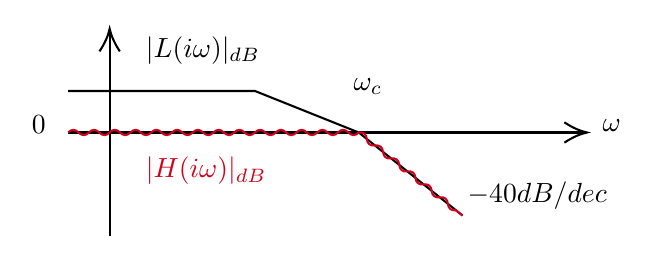
\begin{tikzpicture}[x=0.75pt,y=0.75pt,yscale=-1,xscale=1]
		%uncomment if require: \path (0,122); %set diagram left start at 0, and has height of 122
		
		\draw    (140,60) -- (388,60) ;
		\draw [shift={(390,60)}, rotate = 180] [color={rgb, 255:red, 0; green, 0; blue, 0 }  ][line width=0.75]    (10.93,-4.9) .. controls (6.95,-2.3) and (3.31,-0.67) .. (0,0) .. controls (3.31,0.67) and (6.95,2.3) .. (10.93,4.9)   ;
		\draw    (160,110) -- (160,12) ;
		\draw [shift={(160,10)}, rotate = 450] [color={rgb, 255:red, 0; green, 0; blue, 0 }  ][line width=0.75]    (10.93,-4.9) .. controls (6.95,-2.3) and (3.31,-0.67) .. (0,0) .. controls (3.31,0.67) and (6.95,2.3) .. (10.93,4.9)   ;
		\draw [line width=0.75]    (140,40) -- (230,40) -- (280,60) -- (330,100) ;
		\draw [color={rgb, 255:red, 208; green, 2; blue, 27 }  ,draw opacity=1 ][line width=0.75]    (140,60) .. controls (141.67,58.33) and (143.33,58.33) .. (145,60) .. controls (146.67,61.67) and (148.33,61.67) .. (150,60) .. controls (151.67,58.33) and (153.33,58.33) .. (155,60) .. controls (156.67,61.67) and (158.33,61.67) .. (160,60) .. controls (161.67,58.33) and (163.33,58.33) .. (165,60) .. controls (166.67,61.67) and (168.33,61.67) .. (170,60) .. controls (171.67,58.33) and (173.33,58.33) .. (175,60) .. controls (176.67,61.67) and (178.33,61.67) .. (180,60) .. controls (181.67,58.33) and (183.33,58.33) .. (185,60) .. controls (186.67,61.67) and (188.33,61.67) .. (190,60) .. controls (191.67,58.33) and (193.33,58.33) .. (195,60) .. controls (196.67,61.67) and (198.33,61.67) .. (200,60) .. controls (201.67,58.33) and (203.33,58.33) .. (205,60) .. controls (206.67,61.67) and (208.33,61.67) .. (210,60) .. controls (211.67,58.33) and (213.33,58.33) .. (215,60) .. controls (216.67,61.67) and (218.33,61.67) .. (220,60) .. controls (221.67,58.33) and (223.33,58.33) .. (225,60) .. controls (226.67,61.67) and (228.33,61.67) .. (230,60) .. controls (231.67,58.33) and (233.33,58.33) .. (235,60) .. controls (236.67,61.67) and (238.33,61.67) .. (240,60) .. controls (241.67,58.33) and (243.33,58.33) .. (245,60) .. controls (246.67,61.67) and (248.33,61.67) .. (250,60) .. controls (251.67,58.33) and (253.33,58.33) .. (255,60) .. controls (256.67,61.67) and (258.33,61.67) .. (260,60) .. controls (261.67,58.33) and (263.33,58.33) .. (265,60) .. controls (266.67,61.67) and (268.33,61.67) .. (270,60) .. controls (271.67,58.33) and (273.33,58.33) .. (275,60) .. controls (276.67,61.67) and (278.33,61.67) .. (280,60) -- (280,60) .. controls (282.34,59.74) and (283.64,60.78) .. (283.9,63.12) .. controls (284.16,65.47) and (285.46,66.51) .. (287.81,66.25) .. controls (290.15,65.99) and (291.45,67.03) .. (291.71,69.37) .. controls (291.98,71.71) and (293.28,72.75) .. (295.62,72.49) .. controls (297.96,72.24) and (299.26,73.28) .. (299.52,75.62) .. controls (299.79,77.96) and (301.09,79) .. (303.43,78.74) .. controls (305.77,78.48) and (307.07,79.52) .. (307.33,81.86) .. controls (307.59,84.2) and (308.89,85.24) .. (311.23,84.99) .. controls (313.57,84.73) and (314.87,85.77) .. (315.14,88.11) .. controls (315.4,90.45) and (316.7,91.49) .. (319.04,91.23) .. controls (321.39,90.97) and (322.69,92.01) .. (322.95,94.36) .. controls (323.21,96.7) and (324.51,97.74) .. (326.85,97.48) -- (330,100) -- (330,100) ;
		
		\draw (396,52.4) node [anchor=north west][inner sep=0.75pt]    {$\omega $};
		\draw (276,32.4) node [anchor=north west][inner sep=0.75pt]    {$\omega _c$};
		\draw (331,82.4) node [anchor=north west][inner sep=0.75pt]    {$-40\si{dB/dec}$};
		\draw (176,12.4) node [anchor=north west][inner sep=0.75pt]    {$| L(i\omega)| _{\si{dB}}$};
		\draw (176,70.4) node [anchor=north west][inner sep=0.75pt]  [color={rgb, 255:red, 208; green, 2; blue, 27 }  ,opacity=1 ]  {$| H(i\omega)| _{\si{dB}}$};
		\draw (121,50.4) node [anchor=north west][inner sep=0.75pt]    {$0$};
		
		
	\end{tikzpicture}
\end{figure}\FloatBarrier

È un filtro passa-basso, con banda $\{\omega :0< \omega < \omega _c\}$. Questo induce una stima del tempo di risposta. Indurre uno scalino alla $w$ significa chiedere quello specifico valore. Non conosciamo i poli di $H$, ma possiamo fare un esercizio di identificazione. Tipo $0$ e guadagno $0 \si{dB}$, cioè $1$.
\begin{equation*}
	H(s) =\frac{1}{\left(1+\frac{1}{\omega _c} s\right)^2}
\end{equation*}
L'esponente è $2$ perché nell'esempio considerato la pendenza finale è $-40$, in generale è diverso, ma la struttura è quella. Il primo cambio di pendenza è alla $\omega _c$ e la prima ci dice il tempo dominante.
\begin{equation*}
	\boxed{T_R \approx 5T_D =\frac{5}{\omega _c}}
\end{equation*}

\section{Errore a regime}

Consideriamo un sistema asint. stabile. In generale i disturbi presenti saranno dovuti a
\begin{itemize}
	\item la specifica $w(t)$ che richiediamo
	\item un disturbo in uscita $d(t)$
	\item un disturbo di misura $m(t)$ dovuto alla misurazione stessa dell'uscita
\end{itemize}

\begin{figure}[htpb]\centering
	\tikzset{every picture/.style={line width=0.75pt}} %set default line width to 0.75pt        
	
	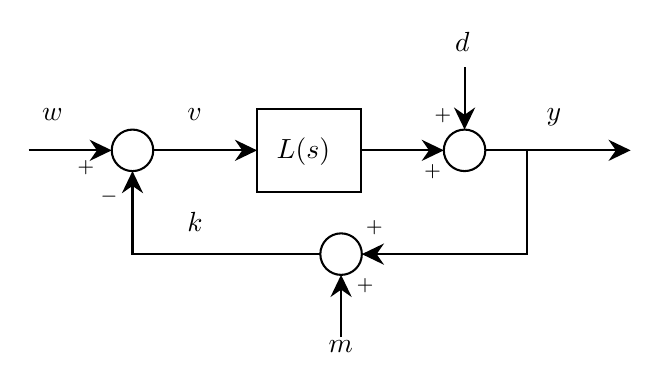
\begin{tikzpicture}[x=0.75pt,y=0.75pt,yscale=-1,xscale=1]
		%uncomment if require: \path (0,194); %set diagram left start at 0, and has height of 194
		
		%Shape: Circle [id:dp4925815313964299] 
		\draw   (140,70) .. controls (140,64.48) and (144.48,60) .. (150,60) .. controls (155.52,60) and (160,64.48) .. (160,70) .. controls (160,75.52) and (155.52,80) .. (150,80) .. controls (144.48,80) and (140,75.52) .. (140,70) -- cycle ;
		\draw    (100,70) -- (137,70) ;
		\draw [shift={(140,70)}, rotate = 180] [fill={rgb, 255:red, 0; green, 0; blue, 0 }  ][line width=0.08]  [draw opacity=0] (10.72,-5.15) -- (0,0) -- (10.72,5.15) -- (7.12,0) -- cycle    ;
		\draw    (160,70) -- (207,70) ;
		\draw [shift={(210,70)}, rotate = 180] [fill={rgb, 255:red, 0; green, 0; blue, 0 }  ][line width=0.08]  [draw opacity=0] (10.72,-5.15) -- (0,0) -- (10.72,5.15) -- (7.12,0) -- cycle    ;
		%Shape: Rectangle [id:dp4347395141873107] 
		\draw   (210,50) -- (260,50) -- (260,90) -- (210,90) -- cycle ;
		%Shape: Circle [id:dp43367543201570435] 
		\draw   (300,70) .. controls (300,64.48) and (304.48,60) .. (310,60) .. controls (315.52,60) and (320,64.48) .. (320,70) .. controls (320,75.52) and (315.52,80) .. (310,80) .. controls (304.48,80) and (300,75.52) .. (300,70) -- cycle ;
		\draw    (260,70) -- (297,70) ;
		\draw [shift={(300,70)}, rotate = 180] [fill={rgb, 255:red, 0; green, 0; blue, 0 }  ][line width=0.08]  [draw opacity=0] (10.72,-5.15) -- (0,0) -- (10.72,5.15) -- (7.12,0) -- cycle    ;
		\draw    (320,70) -- (387,70) ;
		\draw [shift={(390,70)}, rotate = 180] [fill={rgb, 255:red, 0; green, 0; blue, 0 }  ][line width=0.08]  [draw opacity=0] (10.72,-5.15) -- (0,0) -- (10.72,5.15) -- (7.12,0) -- cycle    ;
		\draw    (240.5,120) -- (150,120) -- (150,83) ;
		\draw [shift={(150,80)}, rotate = 450] [fill={rgb, 255:red, 0; green, 0; blue, 0 }  ][line width=0.08]  [draw opacity=0] (10.72,-5.15) -- (0,0) -- (10.72,5.15) -- (7.12,0) -- cycle    ;
		\draw    (310,30) -- (310,57) ;
		\draw [shift={(310,60)}, rotate = 270] [fill={rgb, 255:red, 0; green, 0; blue, 0 }  ][line width=0.08]  [draw opacity=0] (10.72,-5.15) -- (0,0) -- (10.72,5.15) -- (7.12,0) -- cycle    ;
		%Shape: Circle [id:dp3918774555743547] 
		\draw   (240.5,120) .. controls (240.5,114.48) and (244.98,110) .. (250.5,110) .. controls (256.02,110) and (260.5,114.48) .. (260.5,120) .. controls (260.5,125.52) and (256.02,130) .. (250.5,130) .. controls (244.98,130) and (240.5,125.52) .. (240.5,120) -- cycle ;
		\draw    (340,70) -- (340,120) -- (263.5,120) ;
		\draw [shift={(260.5,120)}, rotate = 360] [fill={rgb, 255:red, 0; green, 0; blue, 0 }  ][line width=0.08]  [draw opacity=0] (10.72,-5.15) -- (0,0) -- (10.72,5.15) -- (7.12,0) -- cycle    ;
		\draw    (250.5,160) -- (250.5,133) ;
		\draw [shift={(250.5,130)}, rotate = 450] [fill={rgb, 255:red, 0; green, 0; blue, 0 }  ][line width=0.08]  [draw opacity=0] (10.72,-5.15) -- (0,0) -- (10.72,5.15) -- (7.12,0) -- cycle    ;
		
		\draw (218,62.4) node [anchor=north west][inner sep=0.75pt]    {$L(s)$};
		\draw (105,48.4) node [anchor=north west][inner sep=0.75pt]    {$w$};
		\draw (243,160.4) node [anchor=north west][inner sep=0.75pt]    {$m$};
		\draw (348,48.4) node [anchor=north west][inner sep=0.75pt]    {$y$};
		\draw (122,73.4) node [anchor=north west][inner sep=0.75pt]  [font=\scriptsize]  {$+$};
		\draw (133,87.4) node [anchor=north west][inner sep=0.75pt]  [font=\scriptsize]  {$-$};
		\draw (289,75.4) node [anchor=north west][inner sep=0.75pt]  [font=\scriptsize]  {$+$};
		\draw (294,48.4) node [anchor=north west][inner sep=0.75pt]  [font=\scriptsize]  {$+$};
		\draw (304,11.4) node [anchor=north west][inner sep=0.75pt]    {$d$};
		\draw (261,102.4) node [anchor=north west][inner sep=0.75pt]  [font=\scriptsize]  {$+$};
		\draw (256.5,130.4) node [anchor=north west][inner sep=0.75pt]  [font=\scriptsize]  {$+$};
		\draw (175,48.4) node [anchor=north west][inner sep=0.75pt]    {$v$};
		\draw (175,98.4) node [anchor=north west][inner sep=0.75pt]    {$k$};
		
		
	\end{tikzpicture}
\end{figure}\FloatBarrier

Supponiamo $d(t) ,m(t) ,w(t)$ costanti e calcoliamo l'errore.
\begin{equation*}
	\begin{aligned}
		e      & =w-y              \\
		       & =w-(d+Lv)         \\
		       & =w-(d+L(w-k))     \\
		       & =w-(d+L(w-(m+y))) \\
		       & =w-d+Lm-L(w-y)    \\
		       & =w-d+Lm-Le        \\
		e(1+L) & =w-d+Lm           
	\end{aligned} \ \ \implies \ \ \boxed{e=\frac{1}{1+L} w-\frac{1}{1+L} d+\frac{L}{1+L} m}
\end{equation*}
Studiamola nello spirito della sovrapposizione degli effetti
\begin{itemize}
	\item effetto di $\overline{w}$ costante. I termini delle produttorie nella $L(s)$ non contano nel limite per $s\to 0$\begin{equation*}
	      \begin{aligned}
	      	\overline{e}      & =F(0)\overline{w} =\frac{1}{1+L(0)}\overline{w} =\left(\frac{1}{1+\frac{\mu }{s^h}}\overline{w}\right)_{s=0} =\left(\frac{s^h}{s^h +\mu }\overline{w}\right)_{s=0} \\
	      	                  & =\begin{cases}                                                                                                                                                     
	      	\text{se} \ h=0,  & \frac{1}{1+\mu }\overline{w}                                                                                                                                       \\
	      	\text{se} \ h >0, & 0                                                                                                                                                                  \\
	      	\text{se} \ h< 0, & \overline{w}                                                                                                                                                       
	      	\end{cases}
	      \end{aligned}
	\end{equation*}
	\begin{itemize}
		\item se ha tipo $0$ l'errore può essere abbattuto prendendo $\mu $ grande
		\item se ha tipo $ >0$ l'errore è nullo, cioè ha (almeno) un integratore. Ciò ci fa partire già da fasi negative e ci consuma già $90$ gradi di margine di fase (nel criterio di Bode)
		\item se ha tipo $< 0$, sei nella cacca, non accettabile. D'ora in poi quindi non consideriamo più questi casi, dato che il disturbo non può essere attenuato.
	\end{itemize}
	\item effetto di $\overline{d}$ costante\begin{equation*}
	      \overline{e} =\begin{cases}
	      \text{se} \ h=0, & -\frac{1}{1+\mu }\overline{d}\\
	      \text{se} \ h >0, & 0
	\end{cases}
	\end{equation*}
	\item effetto di $\overline{m}$ costante\begin{equation*}
	      \begin{aligned}
	      	\overline{e}      & =F(0)\overline{m} =\frac{L(0)}{1+L(0)}\overline{m} =\left(\frac{\frac{\mu }{s^h}}{1+\frac{\mu }{s^h}}\overline{m}\right)_{s=0} =\left(\frac{\mu }{s^h +\mu }\overline{m}\right)_{s=0} \\
	      	                  & =\begin{cases}                                                                                                                                                                        
	      	\text{se} \ h=0,  & \frac{\mu }{1+\mu }\overline{m}\xrightarrow{\mu \to \infty }\overline{m}                                                                                                      \\
	      	\text{se} \ h >0, & \overline{m}                                                                                                                                                                          
	      	\end{cases}
	      \end{aligned}
	\end{equation*}\textbf{Nell'errore ritroviamo interamente l'errore di misura}, non siamo in grado di abbatterlo, infatti non dipende dal sistema, non altera il valore dell'uscita.
\end{itemize}

Questa trattazione è stata fatta sull'errore, ma analogamente si può ragionare su come reagisce l'uscita $y$ e giungere a risultati concordi:
\begin{equation*}
	\begin{aligned}
		y      & =d+Lv         \\
		       & =d+L(w-k)     \\
		       & =d+L(w-(m+y)) \\
		       & =d+Lw-Lm-Ly   \\
		y(1+L) & =Lw+d-Lm      
	\end{aligned} \ \ \implies \ \ \boxed{y=\frac{L}{1+L} w+\frac{1}{1+L} d-\frac{L}{1+L} m}
\end{equation*}
Vale poi l'analogo studio dei disturbi a regime.

\section{Disturbo sinusoidale}

Analizziamo cosa succede se il disturbo che consideriamo è sinusoidale. Abbiamo visto che l'errore si può genericamente scrivere come
\begin{equation*}
	e=\frac{1}{1+L} w-\frac{1}{1+L} d+\frac{L}{1+L} m=F_1(s) d_1 +F_2(s) d_2 +F_3(s) d_3
\end{equation*}
Supponiamo quindi che un certo disturbo sia
\begin{equation*}
	d(t) =D\sin(\omega t+T)
\end{equation*}
Allora si dimostra che
\begin{equation}
	\boxed{e_{\infty }(t) =D| F(i\omega)| \sin(\omega t+T+\arg F(i\omega))}
\end{equation}
Se per esempio il termine $F(s)$ fosse 
\begin{equation*}
	F(s) =-\frac{1}{1+L(s)}
\end{equation*}
lo potremmo approssimare come
\begin{equation*}
	| F(i\omega)| =\left| -\frac{1}{1+L(i\omega)}\right| =\frac{1}{| 1+L(i\omega)| } =\begin{cases}
	\text{se} \ | L(i\omega)| \gg 1, & \frac{1}{| L(i\omega)| }\\
	\text{se} \ | L(i\omega)| \ll 1, & 1\ (0\ \si{dB})
	\end{cases}
\end{equation*}
Attenzione che
\begin{equation*}
	\left(\frac{1}{| L(i\omega)| }\right)_{\si{dB}} =20\log\frac{1}{| L(i\omega)| } =-20\log| L(i\omega)| 
\end{equation*}
pertanto prima di $\omega _c$ si ha un ribaltamento nell'approssimazione della $F$.

\begin{figure}[htpb]\centering
	\tikzset{every picture/.style={line width=0.75pt}} %set default line width to 0.75pt        
	
	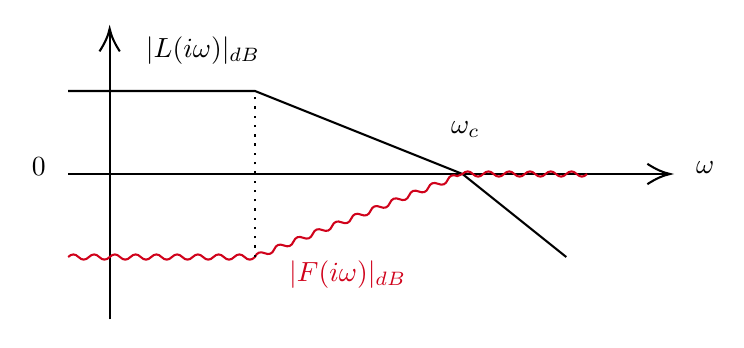
\begin{tikzpicture}[x=0.75pt,y=0.75pt,yscale=-1,xscale=1]
		%uncomment if require: \path (0,163); %set diagram left start at 0, and has height of 163
		
		\draw    (140,80) -- (428,80) ;
		\draw [shift={(430,80)}, rotate = 180] [color={rgb, 255:red, 0; green, 0; blue, 0 }  ][line width=0.75]    (10.93,-4.9) .. controls (6.95,-2.3) and (3.31,-0.67) .. (0,0) .. controls (3.31,0.67) and (6.95,2.3) .. (10.93,4.9)   ;
		\draw    (160,150) -- (160,12) ;
		\draw [shift={(160,10)}, rotate = 450] [color={rgb, 255:red, 0; green, 0; blue, 0 }  ][line width=0.75]    (10.93,-4.9) .. controls (6.95,-2.3) and (3.31,-0.67) .. (0,0) .. controls (3.31,0.67) and (6.95,2.3) .. (10.93,4.9)   ;
		\draw [line width=0.75]    (140,40) -- (230,40) -- (330,80) -- (380,120) ;
		\draw [color={rgb, 255:red, 208; green, 2; blue, 27 }  ,draw opacity=1 ][line width=0.75]    (140,120) .. controls (141.67,118.33) and (143.33,118.33) .. (145,120) .. controls (146.67,121.67) and (148.33,121.67) .. (150,120) .. controls (151.67,118.33) and (153.33,118.33) .. (155,120) .. controls (156.67,121.67) and (158.33,121.67) .. (160,120) .. controls (161.67,118.33) and (163.33,118.33) .. (165,120) .. controls (166.67,121.67) and (168.33,121.67) .. (170,120) .. controls (171.67,118.33) and (173.33,118.33) .. (175,120) .. controls (176.67,121.67) and (178.33,121.67) .. (180,120) .. controls (181.67,118.33) and (183.33,118.33) .. (185,120) .. controls (186.67,121.67) and (188.33,121.67) .. (190,120) .. controls (191.67,118.33) and (193.33,118.33) .. (195,120) .. controls (196.67,121.67) and (198.33,121.67) .. (200,120) .. controls (201.67,118.33) and (203.33,118.33) .. (205,120) .. controls (206.67,121.67) and (208.33,121.67) .. (210,120) .. controls (211.67,118.33) and (213.33,118.33) .. (215,120) .. controls (216.67,121.67) and (218.33,121.67) .. (220,120) .. controls (221.67,118.33) and (223.33,118.33) .. (225,120) .. controls (226.67,121.67) and (228.33,121.67) .. (230,120) -- (230,120) .. controls (230.93,117.83) and (232.47,117.21) .. (234.64,118.14) .. controls (236.81,119.07) and (238.35,118.46) .. (239.28,116.29) .. controls (240.21,114.12) and (241.76,113.5) .. (243.93,114.43) .. controls (246.1,115.36) and (247.64,114.74) .. (248.57,112.57) .. controls (249.5,110.4) and (251.04,109.79) .. (253.21,110.72) .. controls (255.38,111.65) and (256.92,111.03) .. (257.85,108.86) .. controls (258.78,106.69) and (260.33,106.07) .. (262.5,107) .. controls (264.67,107.93) and (266.21,107.31) .. (267.14,105.14) .. controls (268.07,102.97) and (269.61,102.36) .. (271.78,103.29) .. controls (273.95,104.22) and (275.49,103.6) .. (276.42,101.43) .. controls (277.35,99.26) and (278.9,98.64) .. (281.07,99.57) .. controls (283.24,100.5) and (284.78,99.89) .. (285.71,97.72) .. controls (286.64,95.55) and (288.18,94.93) .. (290.35,95.86) .. controls (292.52,96.79) and (294.06,96.17) .. (294.99,94) .. controls (295.92,91.83) and (297.47,91.22) .. (299.64,92.15) .. controls (301.81,93.08) and (303.35,92.46) .. (304.28,90.29) .. controls (305.21,88.12) and (306.75,87.5) .. (308.92,88.43) .. controls (311.09,89.36) and (312.63,88.74) .. (313.56,86.57) .. controls (314.49,84.4) and (316.04,83.79) .. (318.21,84.72) .. controls (320.38,85.65) and (321.92,85.03) .. (322.85,82.86) .. controls (323.78,80.69) and (325.32,80.07) .. (327.49,81) -- (330,80) -- (330,80) .. controls (331.67,78.33) and (333.33,78.33) .. (335,80) .. controls (336.67,81.67) and (338.33,81.67) .. (340,80) .. controls (341.67,78.33) and (343.33,78.33) .. (345,80) .. controls (346.67,81.67) and (348.33,81.67) .. (350,80) .. controls (351.67,78.33) and (353.33,78.33) .. (355,80) .. controls (356.67,81.67) and (358.33,81.67) .. (360,80) .. controls (361.67,78.33) and (363.33,78.33) .. (365,80) .. controls (366.67,81.67) and (368.33,81.67) .. (370,80) .. controls (371.67,78.33) and (373.33,78.33) .. (375,80) .. controls (376.67,81.67) and (378.33,81.67) .. (380,80) .. controls (381.67,78.33) and (383.33,78.33) .. (385,80) .. controls (386.67,81.67) and (388.33,81.67) .. (390,80) -- (390,80) ;
		\draw  [dash pattern={on 0.84pt off 2.51pt}]  (230,120) -- (230,40) ;
		
		\draw (441,72.4) node [anchor=north west][inner sep=0.75pt]    {$\omega $};
		\draw (323,53.4) node [anchor=north west][inner sep=0.75pt]    {$\omega _c$};
		\draw (176,12.4) node [anchor=north west][inner sep=0.75pt]    {$| L(i\omega)| _{\si{dB}}$};
		\draw (245,120.4) node [anchor=north west][inner sep=0.75pt]  [color={rgb, 255:red, 208; green, 2; blue, 27 }  ,opacity=1 ]  {$| F(i\omega)| _{\si{dB}}$};
		\draw (121,70.4) node [anchor=north west][inner sep=0.75pt]    {$0$};
		
		
	\end{tikzpicture}
\end{figure}\FloatBarrier

Una nota importante: se il disturbo è \textbf{somma di uno sinusoidale e uno costante} lo si tratta come sinusoidale e la parte a costante si considera con $\omega =0$ nella formula (9).

\newpage

\textbf{Comandi MATLAB}

\begin{itemize}
	\item \texttt{inv(A)} calcola l’inversa di una matrice
	\item \texttt{SYS = ss(A,B,C,D)} crea il modello di stato a tempo continuo
	\item \texttt{SYS = ss(A,B,C,D,1)} crea il modello di stato a tempo discreto
	\item Per creare il sistema con il modello esterno si può procedere come segue
	      
	      \texttt{num = [10,2]}
	      
	      \texttt{den = poly([-1,-1,-1])} (polinomio con queste radici)
	      
	      \texttt{SYS = tf(num,den)}
	\item \texttt{K = dcgain(SYS)} restituisce il guadagno del sistema a regime
	\item \texttt{poli = roots([1 0.7 0.12 -0.09])} calcola le radici di un polinomio
	\item Per trovare il sistema in forma di stato a partire dalla funzione di trasferimento basta utilizzare il comando tf2ss
	      
	      \texttt{[A,B,C,D] = tf2ss([0 3 -0.1 -0.43],[1 0.7 0.12 -0.09])}
	\item Per \ costruire i sistemi non lineari su simulink si usa il blocco FCN. Questo riceve in ingresso un vettore colonna \texttt{[u(1)…u(n)]}.

	\item Per calcolare la risposta allo scalino:
	      
	      \texttt{[out\_sca,time\_sca] = step(S)} (dove S è il Sistema)
	\item Per calcolare la risposta all’impulso:
	      
	      \texttt{[out\_imp,time\_imp] = impulse(S)}

	\item Per calcolare la matrice di raggiungibilità: \texttt{R = ctrb(A,B)}
	\item Per calcolare la matrice di osservabilità: \texttt{O = obsv(A,C)}
	\item Per calcolare il vettore riga \texttt{k} della legge di controllo:
	      
	      \texttt{k = acker(A, -B, autov\_controllore);}
	\item Per calcolare il vettore colonna \texttt{l} del ricostruttore:
	      
	      \texttt{lT = acker(A', -C', autov\_ricostruttore)}

	\item \texttt{bode(SYS)} disegna i diagrammi di Bode e il range di frequenze è scelto in automatico.
	\item \texttt{bode(SYS,\{WMIN,WMAX\})} disegna i diagrammi di bode nel range di frequenze indicato.
	\item \texttt{bode(SYS,W)} valuta la risposta in frequenza nei punti indicati dal vettore \texttt{W}.
	\item \texttt{bode(SYS1,SYS2,...,W)} disegna i diagrammi di Bode sovrapposti di tutti i sistemi indicati (\texttt{W} è opzionale)\\
	Chiamate:
	      \begin{itemize}
	      	
	      	
	      	\item \texttt{[MOD,FASE] = bode(SYS,W)} e \texttt{[MOD,FASE,W] = bode(SYS)}
	      	      
	      	      Restituiscono le risposte in modulo e argomento (in gradi centigradi) ma non disegnano i diagrammi.
	      	\item Per ottenere i valori di MOD in dB:
	      	      
	      	      \texttt{MODDB = 20*log10(MOD)}
	      \end{itemize}

	\item \texttt{conv} Restituisce i coefficienti del \ polinomio \ prodotto di due polinomi in ingresso. Ad esempio, per i coefficienti di $(1+s)^3$:
	      
	      \texttt{den = conv(conv([1 1],[1 1]),[1 1])}

	\item \texttt{lsim} simula la risposta nel tempo del sistema dinamico per ingressi arbitrari.
	\item \texttt{lsim(SYS,U,T)} simula la risposta di \texttt{SYS} all’ingresso \texttt{U} nel tempo \texttt{T}.
	\item \texttt{lsim(SYS,U,T,X0)} simula la risposta di \texttt{SYS} quando lo stato iniziale è \texttt{X0}, altrimenti è zero di default.
	\item \texttt{lsim(SYS1,SYS2,...,U,T,X0)} simula la risposta di numerosi sistemi in un singolo plot.
	      Chiamate:
	      \begin{itemize}
	      	
	      	
	      	\item \texttt{Y = lsim(SYS,U,T)} restituisce l’uscita \texttt{Y} e non disegna nulla sullo schermo.
	      	\item \texttt{[Y,T,X] = lsim(SYS,U,T,X0)} restituisce \texttt{Y}, il vettore tempo \texttt{T} e i vettori di stato \texttt{X} (in una matrice dove la colonna $i$ è il vettore $x_i(t)$).
	      \end{itemize}

	\item con il comando \texttt{margin} è possibile valutare il margine di fase di $L(s)$.
		\begin{itemize}
			\item Chiamata: \texttt{margin(L)}
		\end{itemize}

	\item \texttt{feedback} collega in retroazione due sistemi.
	      
	      Ad esempio, \texttt{M = feedback(M1,M2)} è il sistema \texttt{y = Mu}
	      
	      \tikzset{every picture/.style={line width=0.75pt}} %set default line width to 0.75pt        
	      
	      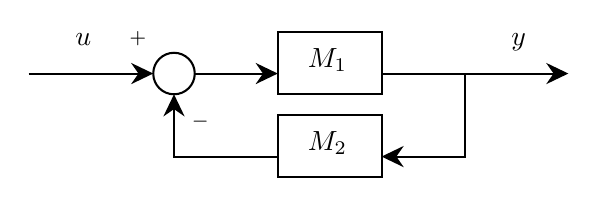
\begin{tikzpicture}[x=0.75pt,y=0.75pt,yscale=-1,xscale=1]
	      	%uncomment if require: \path (0,87); %set diagram left start at 0, and has height of 87
	      	
	      	%Shape: Rectangle [id:dp4706732585641531] 
	      	\draw   (240,10) -- (290,10) -- (290,40) -- (240,40) -- cycle ;
	      	%Shape: Rectangle [id:dp4814034835253058] 
	      	\draw   (240,50) -- (290,50) -- (290,80) -- (240,80) -- cycle ;
	      	\draw    (200,30) -- (237,30) ;
	      	\draw [shift={(240,30)}, rotate = 180] [fill={rgb, 255:red, 0; green, 0; blue, 0 }  ][line width=0.08]  [draw opacity=0] (10.72,-5.15) -- (0,0) -- (10.72,5.15) -- (7.12,0) -- cycle    ;
	      	\draw    (290,30) -- (377,30) ;
	      	\draw [shift={(380,30)}, rotate = 180] [fill={rgb, 255:red, 0; green, 0; blue, 0 }  ][line width=0.08]  [draw opacity=0] (10.72,-5.15) -- (0,0) -- (10.72,5.15) -- (7.12,0) -- cycle    ;
	      	\draw    (330,30) -- (330,70) -- (293,70) ;
	      	\draw [shift={(290,70)}, rotate = 360] [fill={rgb, 255:red, 0; green, 0; blue, 0 }  ][line width=0.08]  [draw opacity=0] (10.72,-5.15) -- (0,0) -- (10.72,5.15) -- (7.12,0) -- cycle    ;
	      	%Shape: Circle [id:dp3714411856310509] 
	      	\draw   (180,30) .. controls (180,24.48) and (184.48,20) .. (190,20) .. controls (195.52,20) and (200,24.48) .. (200,30) .. controls (200,35.52) and (195.52,40) .. (190,40) .. controls (184.48,40) and (180,35.52) .. (180,30) -- cycle ;
	      	\draw    (240,70) -- (190,70) -- (190,43) ;
	      	\draw [shift={(190,40)}, rotate = 450] [fill={rgb, 255:red, 0; green, 0; blue, 0 }  ][line width=0.08]  [draw opacity=0] (10.72,-5.15) -- (0,0) -- (10.72,5.15) -- (7.12,0) -- cycle    ;
	      	\draw    (120,30) -- (177,30) ;
	      	\draw [shift={(180,30)}, rotate = 180] [fill={rgb, 255:red, 0; green, 0; blue, 0 }  ][line width=0.08]  [draw opacity=0] (10.72,-5.15) -- (0,0) -- (10.72,5.15) -- (7.12,0) -- cycle    ;
	      	
	      	\draw (253,16.4) node [anchor=north west][inner sep=0.75pt]    {$M_1$};
	      	\draw (253,56.4) node [anchor=north west][inner sep=0.75pt]    {$M_2$};
	      	\draw (351,9.4) node [anchor=north west][inner sep=0.75pt]    {$y$};
	      	\draw (141,9.4) node [anchor=north west][inner sep=0.75pt]    {$u$};
	      	\draw (167,8.4) node [anchor=north west][inner sep=0.75pt]  [font=\scriptsize]  {$+$};
	      	\draw (197,48.4) node [anchor=north west][inner sep=0.75pt]  [font=\scriptsize]  {$-$};	      	
	      \end{tikzpicture}

	\item Per visualizzare i poli e gli zeri del sistema sotto controllo con guadagno $\mu $:\\
		\texttt{pzmap(SYS), axis([-a a -b b])}
\end{itemize}
